% **************************************************
% Document Class Definition
% **************************************************
\documentclass[%
    paper=A4,               % paper size --> A4 is default in Germany
    twoside=true,           % onesite or twoside printing
    openright,              % doublepage cleaning ends up right side
    parskip=full,           % spacing value / method for paragraphs
    chapterprefix=true,     % prefix for chapter marks
    12pt,                   % font size
    headings=normal,        % size of headings
    bibliography=totoc,     % include bib in toc
    listof=totoc,           % include listof entries in toc
    titlepage=on,           % own page for each title page
    captions=tableabove,    % display table captions above the float env
    draft=false,            % value for draft version
]{scrreprt}%


% **************************************************
% Setup YOUR thesis document in this file !
% **************************************************
% !TEX root = my-thesis.tex

% **************************************************
% Extra packages
% **************************************************
\usepackage{multicol}
%\usepackage{epstopdf}
%\setlength{\belowcaptionskip}{-10pt}
\usepackage{booktabs}

% Para hacer una pagina horizontal. Uso: \begin{landscape} xxxx \end{lanscape}
\usepackage{lscape} 
% Para incluir paginas PDF. Uso:
% \includepdf[pages={1}]{tuarchivo.pdf}
\usepackage{pdfpages}
% Para introducir url's con formato. Uso: \url{http://www.google.es}
\usepackage{url}
% Amplia muchas funciones graficas de latex
\usepackage{graphicx}
% Paquete que añade el hipervinculo en referencias dentro del documento, indice, etc
% Se define sin bordes alrededor. Uso: \ref{tulabel}
\usepackage{hyperref}
%\usepackage[pdfborder={000}]{hyperref}
\usepackage{float}
\usepackage{placeins}
\usepackage{afterpage}
\usepackage{verbatim}
% Paquete para condicionales avanzados
\usepackage{xstring,xifthen}
% Paquete para realizar cálculos en el código
\usepackage{calc}
% Para rotar tablas o figuras o su contenido
\usepackage{rotating} 
% Para incluir comentarios en el texto. El parámetro 'disable' oculta todas las notas.
% USO: \todo{tutexto}
\usepackage[textsize=tiny,spanish,shadow,textwidth=2cm]{todonotes}

\usepackage{subcaption} % Para poder realizar subfiguras
%\usepackage{caption} % Para aumentar las opciones de diseño
% Nombres de figuras, tablas, etc, en negrita la numeración, todo con letra small
\captionsetup{labelfont={bf,small},textfont=small}
% Paquete para modificar los espacios arriba y abajo de una figura o tabla
\usepackage{setspace}
% Define el espacio tanto arriba como abajo de las figuras, tablas
\setlength{\intextsep}{5mm}
% Para ajustar tamaños de texto de toda una tabla o grafica
% Uso: {\scalefont{0.8} \begin{...} \end{...} }
\usepackage{scalefnt}

\usepackage{mathtools}
\DeclarePairedDelimiter\ceil{\lceil}{\rceil}
\DeclarePairedDelimiter\floor{\lfloor}{\rfloor}
\DeclareMathOperator*{\argmin}{arg\,min}
\providecommand{\abs}[1]{\lvert#1\rvert}

\usepackage{svg}

\usepackage{multirow}

\usepackage[12pt]{moresize}


% **************************************************
% Files' Character Encoding
% **************************************************
\PassOptionsToPackage{utf8}{inputenc}
\usepackage{inputenc}


% **************************************************
% Information and Commands for Reuse
% **************************************************
\newcommand{\thesisTitle}{Estrategia Evolutiva para Diseñar Redes Neuronales Convolucionales}
\newcommand{\thesisName}{Sergio Martínez Hamdoun}
\newcommand{\thesisSubject}{Trabajo Fin de Máster}
\newcommand{\thesisDate}{28 de Junio de 2021}
\newcommand{\thesisVersion}{Documento Final}

\newcommand{\thesisFirstReviewer}{Ángela María Ribeiro Seijas}
\newcommand{\thesisFirstReviewerUniversity}{\protect{Universidad Politécnica de Madrid}}
\newcommand{\thesisFirstReviewerDepartment}{Centro de Automática y Robótica}

\newcommand{\thesisSecondReviewer}{Jeremy Karouta}
\newcommand{\thesisSecondReviewerUniversity}{\protect{Universidad Politécnica de Madrid}}
\newcommand{\thesisSecondReviewerDepartment}{Centro de Automática y Robótica}

\newcommand{\thesisFirstSupervisor}{Jane Doe}
\newcommand{\thesisSecondSupervisor}{John Smith}

\newcommand{\thesisUniversity}{\protect{Universidad Politécnica de Madrid}}
\newcommand{\thesisUniversityDepartment}{Department of Clean Thesis Style}
\newcommand{\thesisUniversityInstitute}{Institute for Clean Thesis Dev}
\newcommand{\thesisUniversityGroup}{Clean Thesis Group (CTG)}
\newcommand{\thesisUniversityCity}{Madrid}
\newcommand{\thesisUniversityStreetAddress}{Street address}
\newcommand{\thesisUniversityPostalCode}{Postal Code}


% **************************************************
% Debug LaTeX Information
% **************************************************
%\listfiles

% **************************************************
% Load and Configure Packages
% **************************************************
\usepackage[spanish]{babel} % babel system, adjust the language of the content
\PassOptionsToPackage{% setup clean thesis style
    figuresep=endash,%
    sansserif=false,%
    hangfigurecaption=true,%
    hangsection=true,%
    hangsubsection=true,%
    colorize=full,%
    colortheme=bluegreen,% bluemagenta
    bibsys=bibtex,%
    bibfile=bib-refs,%
    bibstyle=numeric ,%
    wrapfooter=false,%
}{cleanthesis}
\usepackage{cleanthesis}

\hypersetup{% setup the hyperref-package options
    pdftitle={\thesisTitle},    %   - title (PDF meta)
    pdfsubject={\thesisSubject},%   - subject (PDF meta)
    pdfauthor={\thesisName},    %   - author (PDF meta)
    plainpages=false,           %   -
    colorlinks=false,           %   - colorize links?
    pdfborder={0 0 0},          %   -
    breaklinks=true,            %   - allow line break inside links
    bookmarksnumbered=true,     %
    bookmarksopen=true          %
}




\newcommand{\sergio}[1]{{\color{magenta}\textit{\textsc{\textbf{}} #1}}}
\newcommand{\angela}[1]{{\color{green}\textit{\textsc{\textbf{}} #1}}}
\newcommand{\jeremy}[1]{{\color{red}\textit{\textsc{\textbf{}} #1}}}

% **************************************************
% Document CONTENT
% **************************************************
\begin{document}

% --------------------------
% rename document parts
% --------------------------
%\renewcaptionname{ngerman}{\figurename}{Abb.}
%\renewcaptionname{ngerman}{\tablename}{Tab.}
%\renewcaptionname{english}{\figurename}{Fig.}
%\renewcaptionname{english}{\tablename}{Tab.}
\renewcaptionname{spanish}{\figurename}{Fig.}
\renewcaptionname{spanish}{\tablename}{Tab.}

%Cambiar Cuadros por Tablas y lista de tablas
\renewcommand{\listtablename}{Índice de tablas} 

% --------------------------
% Front matter
% --------------------------
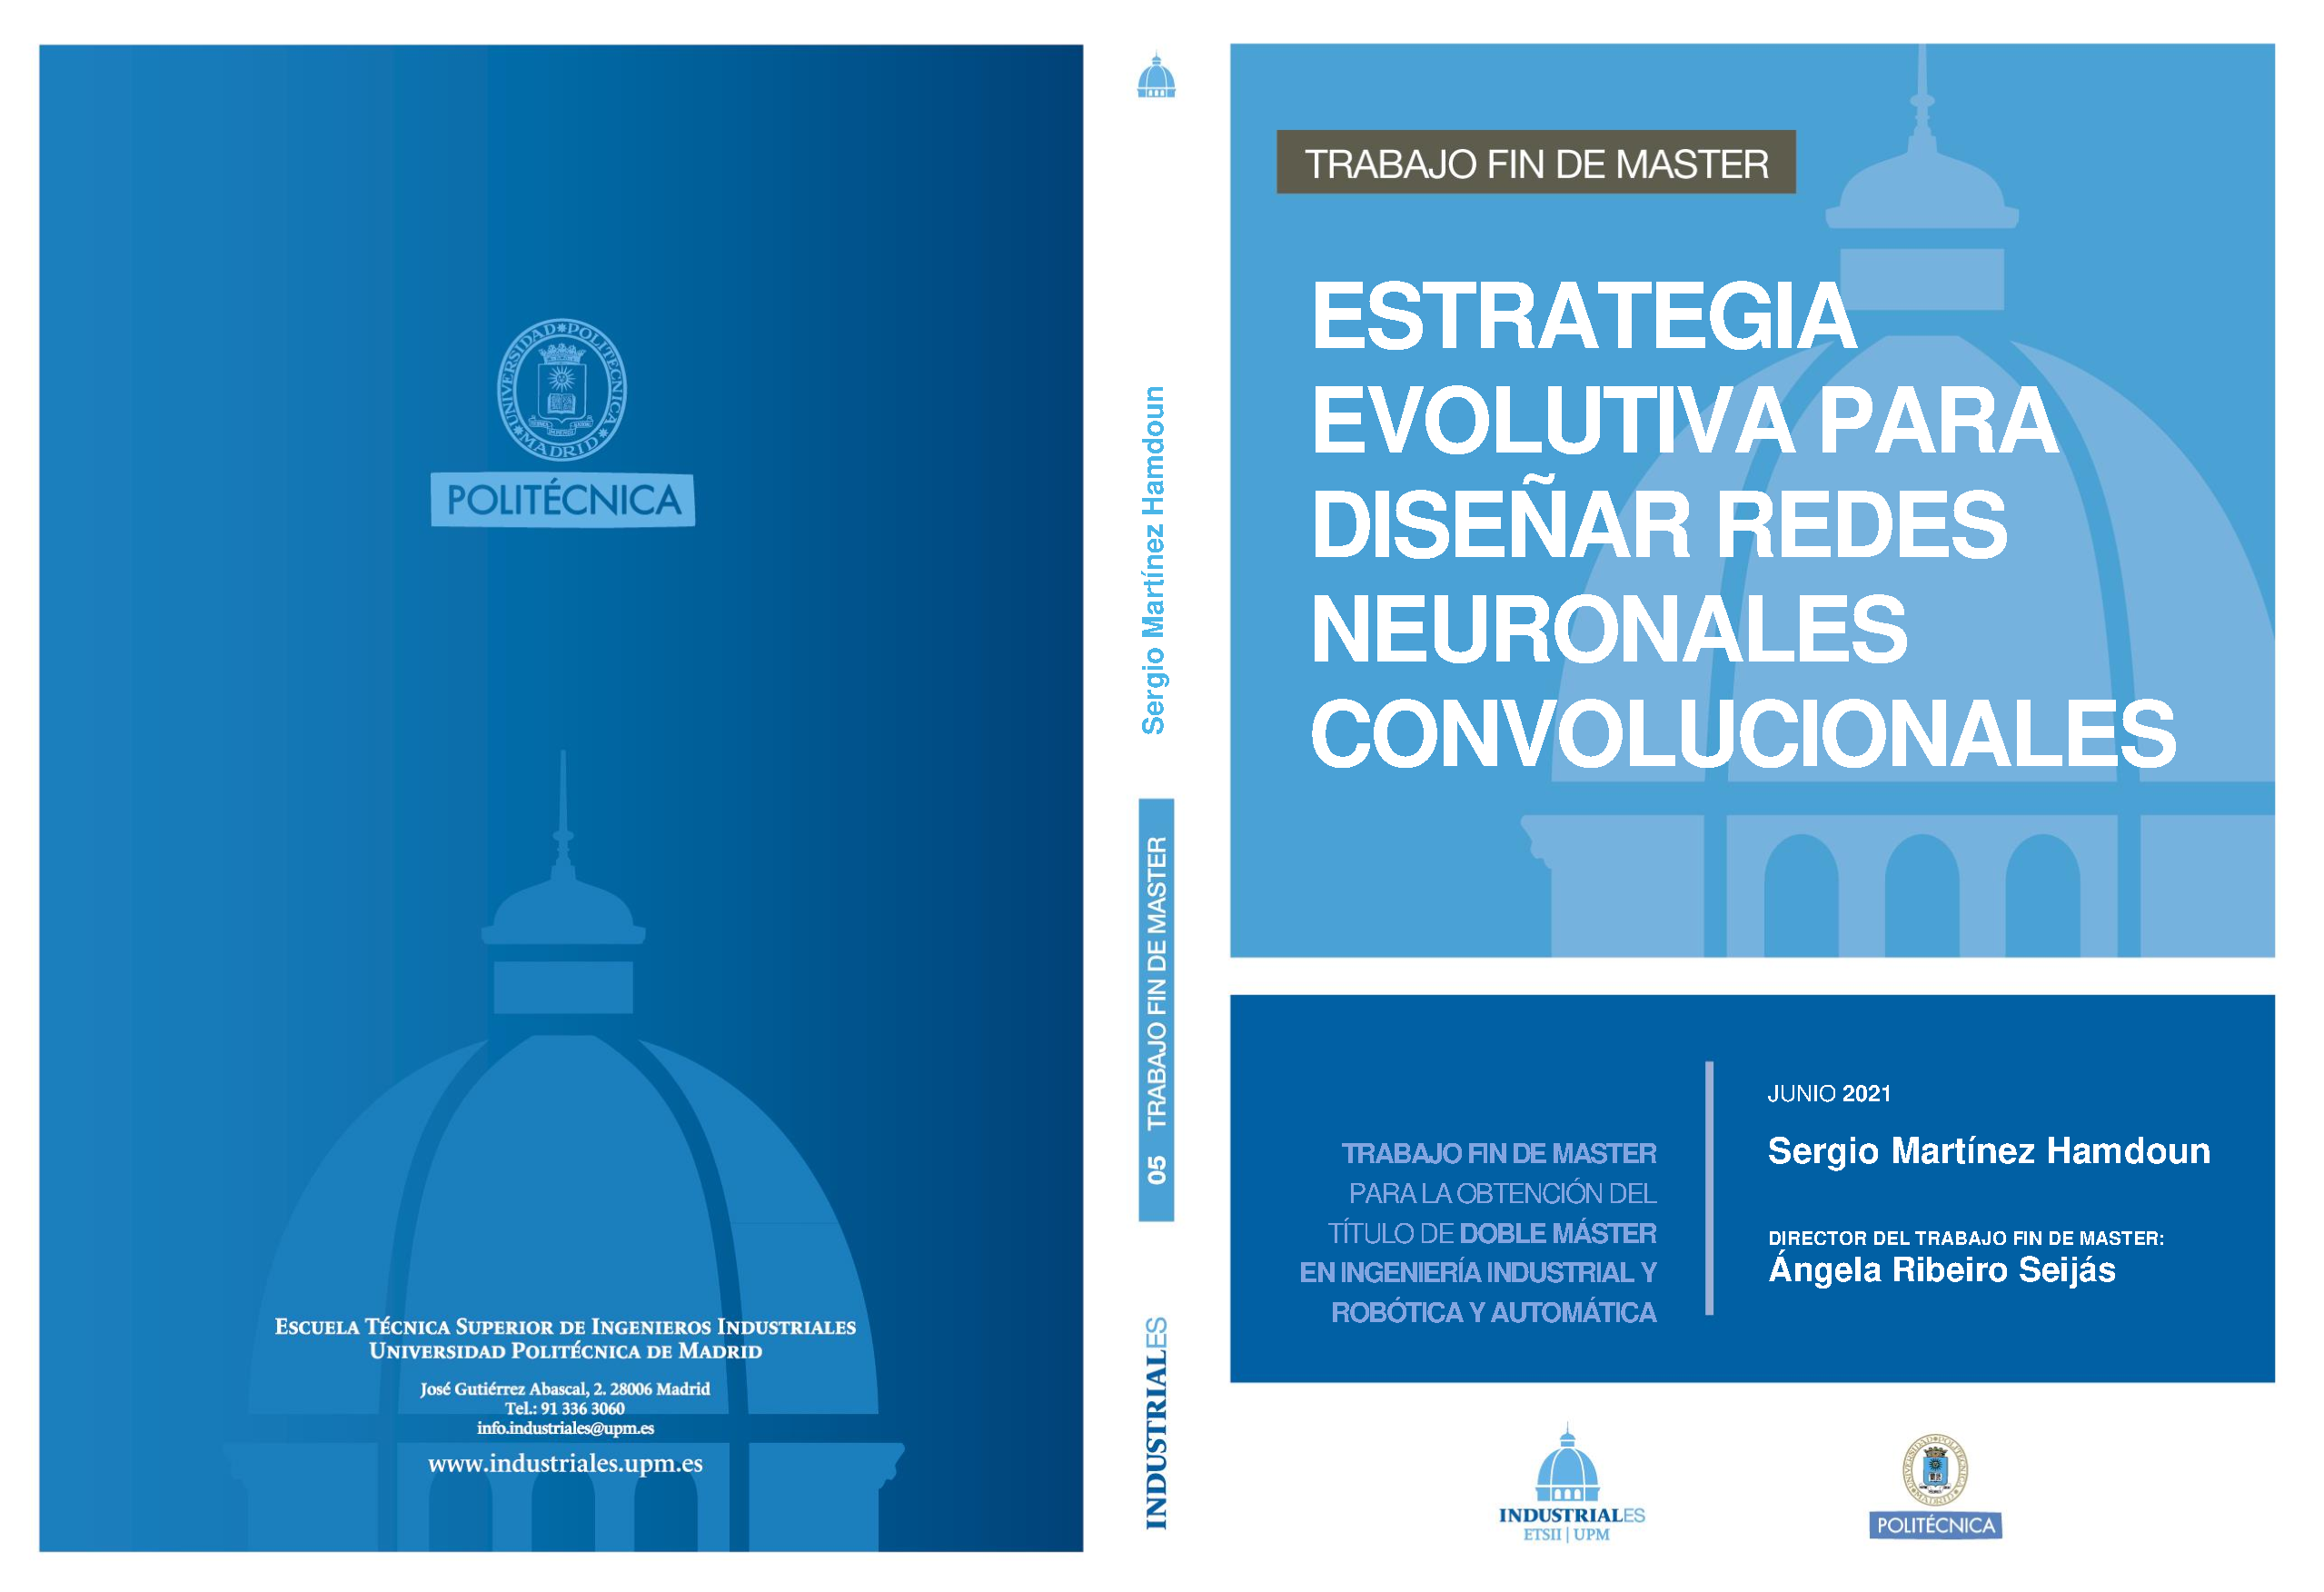
\includepdf[pages=-, fitpaper]{misc/PORTADA_Trabajo_Fin_de_Master.pdf}

\cleardoublepage

\pagenumbering{Roman}			% roman page numbing (invisible for empty page style)
\pagestyle{empty}				% no header or footers
% !TEX root = ../my-thesis.tex
%
% ------------------------------------  --> cover title page
%\begin{titlepage}
%	\pdfbookmark[0]{Cover}{Cover}
%	\flushright
%	\hfill
%	\vfill
%	{\LARGE\thesisTitle \par}
%	\rule[5pt]{\textwidth}{.4pt} \par
%	{\Large\thesisName}
%	\vfill
%	\textit{\large\thesisDate} \\
%	Version: \thesisVersion
%\end{titlepage}


% ------------------------------------  --> main title page
\begin{titlepage}
	\pdfbookmark[0]{Titlepage}{Titlepage}
	\tgherosfont
	\centering
	%\phatom{.}
	
\includegraphics[width=5cm]{figuras/logos/logo_upm_crop.png} \\[1mm]
	{\Large \textbf{Universidad Politécnica de Madrid}}\\[1mm]
	{\large Escuela Técnica Superior de Ingenieros Industriales}\\[10mm]
	

	\hrulefill
	\vfill
    
	{\LARGE \MakeUppercase{\thesisSubject}} \\[5mm]
	{\Huge \color{ctcolortitle}\textbf{\thesisTitle} \\[10mm]}
	%{\Large \thesisName} \\

	\begin{minipage}[t]{.27\textwidth}
		\raggedleft
		\textit{Autor}
	\end{minipage}
	\hspace*{15pt}
	\begin{minipage}[t]{.65\textwidth}
		{\Large \thesisName} \\
	  	{\small Doble Máster en Ingeniería Industrial \\y Automática y Robótica} \\[-1mm]
		% {\small Universidad Politécnica de Madrid}
	\end{minipage} \\[5mm]
	\vfill
	\hrulefill
	
	\vspace{10mm}
	
	\begin{minipage}[t]{.27\textwidth}
		\raggedleft
		\textit{Tutor}
	\end{minipage}
	\hspace*{15pt}
	\begin{minipage}[t]{.65\textwidth}
		{\Large \thesisFirstReviewer} \\
	  	{\small \thesisFirstReviewerDepartment} \\[-1mm]
		% {\small \thesisFirstReviewerUniversity}
	\end{minipage} \\[10mm]
	
% 	\begin{minipage}[t]{.27\textwidth}
% 		\raggedleft
% 		\textit{Co-tutor}
% 	\end{minipage}
% 	\hspace*{15pt}
% 	\begin{minipage}[t]{.65\textwidth}
% 		{\Large \thesisSecondReviewer} \\
% 	  	{\small \thesisSecondReviewerDepartment} \\[-1mm]
% 		{\small \thesisSecondReviewerUniversity}
% 	\end{minipage} \\[20mm]
	
%	\begin{minipage}[t]{.27\textwidth}
%		\raggedleft
%		\textit{Supervisors}
%	\end{minipage}
%	\hspace*{15pt}
%	\begin{minipage}[t]{.65\textwidth}
%		\thesisFirstSupervisor\ and \thesisSecondSupervisor
%	\end{minipage} \\[10mm]
    
    \thesisDate
    \vfill
    
    %\begin{multicols}{2}
    %\vfill
	%\includegraphics[width=3cm]{figuras/logos/uma_color.png} \\[2mm]
	%\columnbreak
	%\vfill
	
	%\includegraphics[width=4.5cm]{figuras/logos/industriales.png}
    %\end{multicols}
    
    

\end{titlepage}


% ------------------------------------  --> lower title back for single page layout
%\hfill
%\vfill
%{
%	\small
%	\textbf{\thesisName} \\
%	\textit{\thesisTitle} \\
%	\thesisSubject, \thesisDate \\
%	Reviewers: \thesisFirstReviewer\ and \thesisSecondReviewer \\
%	Supervisors: \thesisFirstSupervisor\ and \thesisSecondSupervisor \\[1.5em]
%	\textbf{\thesisUniversity} \\
%	\textit{\thesisUniversityGroup} \\
%	\thesisUniversityInstitute \\
%	\thesisUniversityDepartment \\
%	\thesisUniversityStreetAddress \\
%	\thesisUniversityPostalCode\ and \thesisUniversityCity
%}
		% INCLUDE: all titlepages
\cleardoublepage

\pagestyle{plain}				% display just page numbers
% !TEX root = ../my-thesis.tex
%
% \pdfbookmark[0]{Resumen}{Resumen}
\chapter*{Resumen}
\addcontentsline{toc}{chapter}{RESUMEN}
\label{sec:abstract}
\vspace*{-10mm}
% ------------------------------------------------------------------------------

La agricultura extensiva en la actualidad, es una actividad impresionable encargada de proporcionar alimentación a la población mundial. Pero esta, presenta graves problemas de carácter medioambiental, de cara a la conservación del planeta, como son la contaminación de aguas por empleo indiscriminado de agentes químicos para el tratamiento plagas y de las denominadas malas hierbas. Además de este, presenta otros problemas, como grandes costes asociados a estas técnicas y rendimientos bajos de las cosechas.

Para ello, la agricultura de precisión propone técnicas por las cuales se apliquen correctivos de forma selectiva en función de las necesidades de cada zona del campo. Estas requieren técnicas automatizadas, como las de objeto de este trabajo, para la detección y clasificación de malas hierbas.

Algunas técnicas de las propuestas a día de hoy se basan en imágenes RGB que son procesadas y clasificadas por Redes Neuronales Convolucionales de propósito general. Estas, a pesar de su gran rendimiento en este tipo de tareas, presentan grandes deficiencias debido a su arquitectura generalista, como su tamaño o el gran coste computacional y los grandes conjuntos de imágenes etiquetadas que son necesarias para su entrenamiento.

En base a todo lo anterior, este trabajo propone demostrar la hipótesis que, empleando algoritmos de optimización como los Algoritmos Evolutivos, se pueden encontrar arquitecturas más eficientes desde el punto de vista de tamaño, tiempo de entrenamiento y requerimiento de grandes conjuntos de datos, que puedan competir en desempeño, con las arquitectura de redes que son empleadas en la actualidad.

\newpage

% ------------------------------------------------------------------------------
\vspace*{10mm}

{\usekomafont{chapter}Palabras clave}\label{sec:palabras-clave} \\ 
% ------------------------------------------------------------------------------

Robótica, Visión por computador, Visión artificial, Inteligencia Artificial, Redes Neuronales Artificiales, Redes Neuronales Convolucionales, Algoritmos Evolutivos, Algoritmos Genéticos

% ------------------------------------------------------------------------------
\vspace*{10mm}

{\usekomafont{chapter}Códigos UNESCO}\label{sec:codigos_unesco} \\ 

\begin{itemize}
    \item 120302: Lenguajes Algorítmicos
    \item 120304: Inteligencia Artificial
    \item 120308: Código y Sistemas de Codificación
    \item 120903: Análisis de datos
    \item 120905: Análisis y Diseño de experimentos
    \item 220925: Tratamiento digital de imágenes
    \item 220310: Redes Neuronales
    \item 330419: Robótica
    \item 331101: Tecnología de la automatización
    \item 521201: Agricultura, Silvicultura, Pesca
\end{itemize}

% ------------------------------------------------------------------------------
% %{\usekomafont{chapter}Abstract}\label{sec:abstract2} \\
% % \pdfbookmark[0]{Abstract}{Abstract}

%\cleardoublepage
% \chapter*{Abstract}
% \addcontentsline{toc}{chapter}{ABSTRACT}
% \label{sec:abstract2}
% \vspace*{-10mm}
% % ------------------------------------------------------------------------------

% Aquí va el Resumen en inglés
% [...]


% % ------------------------------------------------------------------------------
% \vspace*{10mm}

% {\usekomafont{chapter}Keywords}\label{sec:keywords} \\ 
% % ------------------------------------------------------------------------------

% Keywords en inglés
% [...]

% % ------------------------------------------------------------------------------		% INCLUDE: the abstracts (english and german)
\cleardoublepage

\setcounter{tocdepth}{2}		% define depth of toc
\tableofcontents				% display table of contents
\cleardoublepage

% --------------------------
% Body matter
% --------------------------
\pagenumbering{arabic}			% arabic page numbering
\setcounter{page}{1}			% set page counter
\pagestyle{maincontentstyle} 	% fancy header and footer

% !TEX root = ../my-thesis.tex
%
\chapter{INTRODUCCIÓN}
\label{sec:intro}
    
En este capítulo se tratará de realizar una breve introducción al trabajo realizado. Se presentará la motivación de este trabajo, que objetivos se persiguen y la estructura que mantendrá el documento.\\

\section{Motivación}

La automática y la robótica, son tecnologías cada vez más presentes en gran cantidad de procesos industriales que resultaban ser altamente repetitivos para las personas, consiguiendo una mejora considerable en el rendimiento y la productividad de estos.

Uno de los ámbitos donde está entrando con fuerza en los últimos años es el de la agricultura, donde existen espacios de mejora debido al desarrollo de las nuevas tecnologías y a la aparición de grandes intereses económicos, sociales y medioambientales, propician un gran avance de esta. Una rama de la agricultura que fomenta la introducción de este tipo de desarrollos, es la agricultura de precisión, que promete explotar los cultivos consiguiendo un mayor desempeño de estos.

Dentro de la agricultura de precisión se pueden encontrar tareas como la detección, clasificación y eliminación de malas hierbas, que vienen a mejorar las técnicas extensivas actuales donde se localizan grandes deficiencias que afectan a los costes, a la productividad y a la calidad de la cosecha.

En las fases de detección y clasificación, actualmente se cuentan con varias soluciones, donde las más extendidas se basan en el uso de Redes Neuronales Convolucionales genéricas, debido a su gran desempeño. Esta solución, cuenta con varios desventajas, como son el tamaño de estas redes, grandes requerimientos computacionales y la necesidad de enormes conjuntos de datos de entrenamiento.

Por lo tanto, este trabajo viene a dar respuesta a esta problemática, tratando de diseñar nuevas arquitecturas que se adapten de mejor manera al problema de clasificación propuesto, empleando técnicas de optimización, como son las basadas en estrategias evolutivas. Estas se esperan que suplan las deficiencias encontradas en las arquitecturas de las Redes Neuronales Convolucionales más extendidas en la actualidad.

\section{Objetivos}

Este trabajo tiene como objetivo final la creación de un algoritmo basado en estrategias evolutivas para diseñar redes neuronales convolucionales, además de su ejecución y estudio de los resultados obtenidos para la verificación de la hipótesis realizada.

Para la obtención del objetivo final anteriormente comentado, se establecen una serie de objetivos parciales que han de ser alcanzados:

\begin{itemize}

    \item Familiarización con el desarrollo de técnicas de optimización basadas en estrategias evolutivas.
    
    \item Estudio de la arquitecturas y funcionamiento de las redes neuronales convolucionales desarrolladas en la actualidad.
    
    \item Diseño y optimización de algoritmo de generación de arquitecturas de redes neuronales convolucionales basado en estrategias evolutivas.
    
    \item Implantación y ejecución del algoritmo en infraestructura de computación de alto rendimiento de forma remota.
    
    \item Análisis y comparación de los individuos resultado de la ejecución del algoritmo.
    
    \item Verificación de la hipótesis establecida sobre el método de diseño propuesto.
    
\end{itemize}

\section{Estructura}

La estructura de este documento, se basa en seis puntos diferenciados, donde se pretende dar una visión global del trabajo y de las investigaciones realizadas durante la elaboración del mismo.

\begin{itemize}

    \item En primer lugar, se presenta el \textbf{estado del arte} de las problemáticas actuales existentes en la agricultura. Más específicamente, se desarrolla sobre las técnicas de clasificación de malas hierbas que se localizan bajo el paraguas de la agricultura de precisión, localizando las deficiencias que estas tienen.
    
    \item En segundo lugar, se introducen unas \textbf{bases teóricas} que serán necesarias para la comprensión en mayor o menor medida del trabajo desarrollado en este documento.
    
    \item En tercer lugar, una vez conocidas como funcionan los algoritmos que son estudiados, se localiza \textbf{el problema} que motiva el trabajo y se desarrolla la hipótesis que ha de ser verificada durante el desarrollo de este.
    
    \item En cuarto lugar, se realiza el desarrollo de \textbf{la implementación} realizada para la resolución de este problema, tratando de hacer viable la ejecución posterior de esta para la verificación de la hipótesis propuesta.
    
    \item En quinto lugar, se realizan una serie de \textbf{experimentos} y se comentan los \textbf{resultados} obtenidos de la ejecución de la implementación realizada, de manera que se respondan las cuestiones que motivaban el desarrollo de este trabajo.
    
    \item Finalmente, se presentan \textbf{las conclusiones}, donde se exponen las lecciones aprendidas del desarrollo y obtención de resultados durante la investigación, presentando además unas \textbf{líneas futuras}, donde se expliquen que partes de esta podrían ser interesantes de ampliación o estudio en más profundidad.
    
\end{itemize}
  % INCLUDE: introducción
% !TEX root = ../my-thesis.tex
%
\chapter{ESTADO DEL ARTE}
\label{sec:estado del arte}

En este capítulo se tratará de realizar una revisión del estado del arte. Se tocará el estado actual en el que se encuentra la agricultura, la tendencia hacia técnicas de agricultura de precisión. De aquí, se desarrollará la importancia de discriminar entre diferentes tipos de vegetación para su tratamiento individualizado y se verán cuales han sido las tecnologías y técnicas empleadas históricamente para este proceso.

\section{Agricultura}

La agricultura es la actividad ocupada en el cultivo del suelo y la recogida posterior de las cosechas; es una de las grandes invenciones del hombre, que permitió a la civilización un acceso sencillo a los alimentos, permitiendo pasar a sociedades sedentarias como las que conocemos en la actualidad. Esta es una de las principales actividades del sector primario.

Durante el desarrollo de la agricultura, se han visto numerosas revoluciones y transformaciones a lo largo de los años, debido al avance de la tecnología y a las necesidades de la población existente en cada zona del planeta. De entre las más recientes, se puede destacar la vivida en la segunda mitad del siglo XX, donde, por un gran crecimiento de la población trajo un aumento en la demanda de alimentos. Es por ello que se tuvieron que implementar nuevas tecnologías en el campo \cite{Shuler2003}, como pudo ser el uso del tractor, tal y como se conoce en la actualidad, lo que supuso una reducción notable de la mano de obra necesaria para el trabajo en el campo. Además, debido a la mejora en químicos como herbicidas y pesticidas o fertilizantes artificiales, la productividad de los cultivos aumentó considerablemente, adaptándose la producción a las necesidades de la época.

Como contrapartida a esto, este tipo de técnicas han supuesto un deterioro muy importante en la calidad del medioambiente con el vertido de este tipo de productos de forma incontrolada.

En la actualidad, tal y como apuntan varios informes \cite{fao_agricultura_2020} \cite{food2004agricultura} en los últimos años por la FAO (\textit{Food and Agriculture Organization of the United Nations}), en los próximos años se podrá observar una gran transformación en la agricultura y en la alimentación de las personas. Esto se debe, en primer lugar, a la necesidad de una agricultura más sostenible con el medio ambiente. En segundo lugar, debido a las notables consecuencias del cambio climático en el planeta, la variabilidad del clima y de las precipitaciones que supondrán un problema que habrá que enfrentar, para lo que será necesaria la transformación de algunas de las técnicas empleadas actualmente. 

Además de todo lo anterior, otro punto a tener en cuenta es el continuo crecimiento poblacional mundial, crecimiento que podrá suponer un problema para el acceso a los alimentos en los próximos años si no es posible encontrar mejores alternativas con las que trabajar el campo.

\section{Agricultura de Precisión}

La agricultura de precisión se basa en la gestión heterogénea de los cultivos con el fin de aumentar la productividad. En este ámbito, se debe analizar la variabilidad de estos durante las diferentes etapas de su desarrollo. Alguno de los ejemplos que se pueden encontrar en este ámbito son: el estimar la densidad de sembrado, analizar y calcular la cantidad adecuada de fertilizantes, aplicar de forma óptima herbicidas para malas hierbas o analizar el estado actual y el rendimiento de los cultivos.

La \textit{International Society of Precision Agriculture} propone otra definición, mucho más exacta: \textit{``La agricultura de precisión es una estrategia de gestión que recoge, procesa y analiza datos temporales, espaciales e individuales y los combina con otras informaciones para respaldar las decisiones de manejo de acuerdo con la variabilidad estimada, y así mejorar la eficiencia en el uso de recursos, la productividad, la calidad, la rentabilidad y la sostenibilidad de la producción agrícola.''} \cite{ispa}

Sus orígenes se remontan a principios de los años 80 en los Estados Unidos \cite{Robert2002}, donde se comienza con el uso de las nuevas tecnologías disponibles para mejorar la aplicación de fertilizantes en cantidades variables según las necesidades de los cultivos. Posteriormente, esto fue extendiéndose a diferentes prácticas y países. 

La principal motivación del uso de agricultura de precisión proviene de la variabilidad de los cultivos, que puede venir dada desde diferentes puntos. Por ejemplo, la variabilidad producida por el entorno en el que está situado el cultivo, la variabilidad producida por las condiciones climáticas o la producida de manera intencional al utilizar fertilizantes.

Actualmente este tipo de técnicas son una realidad, sin embargo siguen existiendo numerosas barreras tecnológicas que se están tratando de erradicar para poder llevar a cabo este tipo de prácticas de forma satisfactoria. Esto se debe a que el número de tecnologías que se involucran dentro de este tipo de agricultura es muy alto, ya que se necesita obtener gran información del campo. En esta se emplean tecnologías como el uso de sistemas de posicionamiento global (GPS), sensores capaces de monitorizar el estado de las plantas o maquinaría capaz de actuar en las zonas objetivo. \cite{Garcia2008}

\begin{figure}
    \centering
    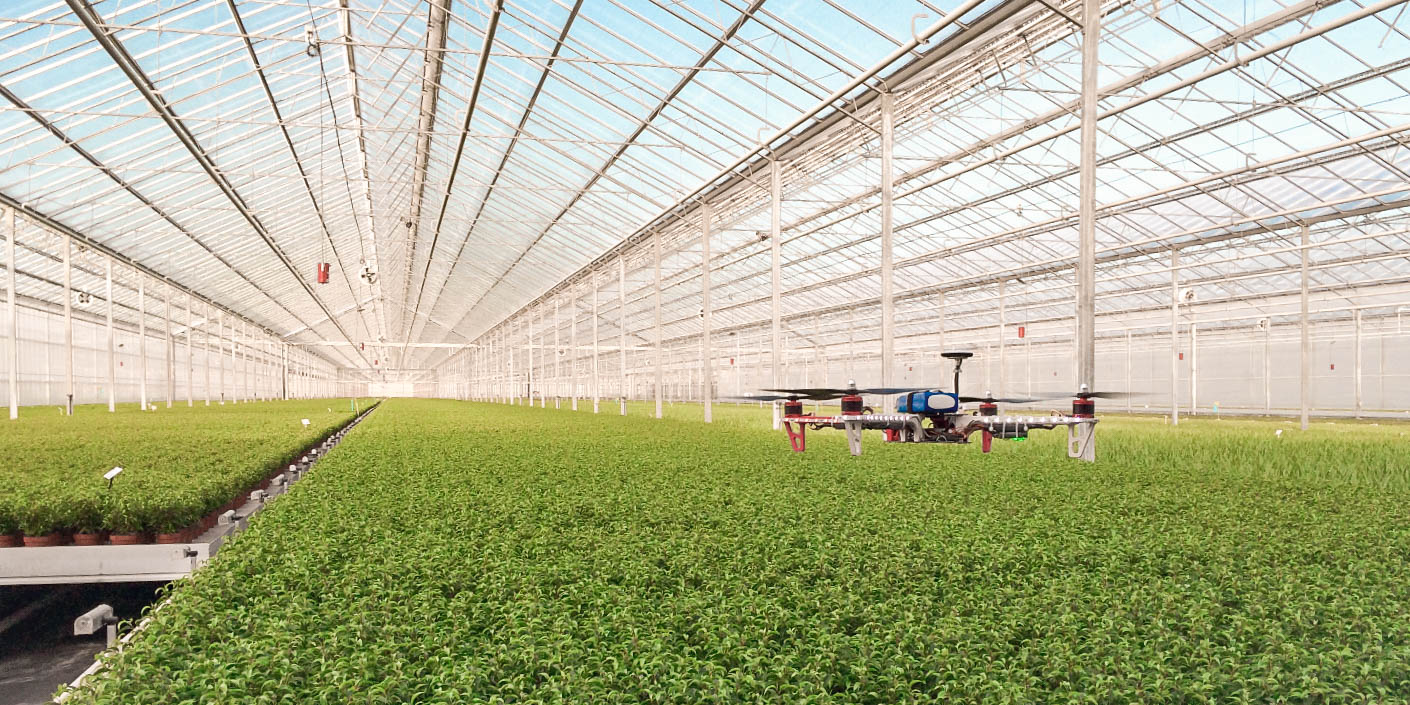
\includegraphics[width=\textwidth]{figuras/estado del arte/dron_inspeccion.jpg}
    \caption{UAV de inspección en Agricultura de Precisión para floricultura en Alemania}
    \label{fig:dron_inspeccion}
\end{figure}

En la Figura \ref{fig:dron_inspeccion}, se puede ver un ejemplo de aplicación de UAVs para la inspección de cultivos de flores en Alemania \cite{job-wizards}. Aquí se combinan tecnologías basadas en el desarrollo de vehículos aéreos no tripulados, la sensorificación a partir de cámaras RGB para la obtención del estado de las plantas, el posicionamiento GPS del vehículo y las comunicaciones en tiempo real de este.

La agricultura de precisión trae asociada numerosos beneficios frente a otros tipos de agricultura. Esta tiene como objetivo principal aportar mas información a los agricultores sobre el estado y la variabilidad de su parcela de cultivo, lo que servirá para conocer cuales son las necesidades reales del campo para su posterior labrado, siembra, riego, fertilización, control de plagas o tratamiento de malas hierbas. Esto trae consigo una mejora en la explotación de la parcela, una reducción en costes y un menor impacto medioambiental.

Enumerando alguno de los beneficios, podemos encontrar los siguientes \cite{Garcia2008}:
\begin{itemize}
    \item Gestión optimizada de las explotaciones.
    \item Reducción de la aplicación de fertilizantes, herbicidas y pesticidas.
    \item Productos con mayor valor nutritivo.
    \item Menor impacto para el medio ambiente.
    \item Reducción en el uso de combustibles para la maquinaria agrícola.
    \item Obtención de información de los cultivos más precisa y con mayor trazabilidad.
\end{itemize}

\section{Tratamiento selectivo contra malas hierbas}

Dentro de la agricultura de precisión, una de las técnicas que adquieren especial importancia, es la aplicación selectiva de agroquímicos \cite{precisionweedmanagement}. Al contrario que los métodos tradicionales, estos métodos proponen ajustar las dosis de tratamiento a las necesidades de cada cultivo, usándose tan solo en las áreas realmente afectadas.

Este área despierta gran interés debido a que es uno de los grandes problemas agrícolas actuales. Esto es así, ya que se estima que puede ser uno de los grandes limitadores dentro de rendimiento potencial de los cultivos. Algunos autores indican que puede llegar a ser incluso hasta un 40\% del potencial total del cultivo \cite{Oerke1999} contando la afectación de otros agentes externos. Las malas hierbas, compiten con las plantas del cultivo por los recursos de la tierra, lo que supone una gran reducción en el rendimiento del terreno.

Algunos experimentos realizados, muestran que el ahorro en agroquímicos puede suponer hasta un 80\% con el uso de estas técnicas selectivas \cite{RUIZ2006} \cite{Hamouz2018ImpactOS} con respecto a las dosis recomendadas, sin necesidad de disminuir en su eficacia ni en el rendimiento de la cosecha. Esto viene traducido en un gran ahorro en los costes de producción.

Además, esto no tiene solo un gran impacto económico, sino que tiene un gran impacto medioambiental, ya que el tratamiento de herbicidas de manera extensiva, causa la contaminación de aguas o la afectación a cultivos cercanos.

Para la aplicación selectiva de tratamiento es necesario una estimación inicial de la cantidad de producto para cada unidad de cultivo \cite{Senay1998}. Para ello, es necesario primeramente, determinar la localización, ver la densidad y clasificar los diferentes tipos de malas hierbas. Con esta información, posteriormente se realiza un selección del modo de actuación adecuada. Finalmente, se aplica de forma selectiva y precisa el tratamiento según las indicaciones estipuladas anteriormente.

\subsection{Técnicas de tratamiento}

Existen diferentes técnicas para el tratamiento de malas hierbas que compiten con el cultivo. Normalmente estas se dividen en cuatro categorías diferenciadas.

\begin{itemize}

    \item \textbf{Técnicas mecánicas:} aquellas que que se aplican directamente sobre las malas hierbas para eliminarlas. Algunas de estas son el entierro, el corte o la quema de esta vegetación.
    
    \item \textbf{Técnicas culturales:} aquellas que no emplean uso de químicos y que se realizan a partir del conocimiento de la propia tierra y el cultivo. Algunas de estas son el labrado, el uso de falsas siembras o el atraso de la fecha de siembra.
    
    \item \textbf{Técnicas biológicas:} aquellas que emplean enemigos naturales para eliminar las malas hierbas. Algunas de estas pueden ser el pastoreo, el uso de micoherbicidas o la aleopatía.
    
    \item \textbf{Técnicas químicas:} aquellas que incluyen principalmente el uso de herbicidas para la eliminación y control de malas hierbas.
    
\end{itemize}

Aún así, desde la aparición durante el siglo XX de herbicidas como ya se comentaba, las técnicas mecánicas han sido relegados a un segundo plano. Esto es debido a su eficacia y su facilidad de uso.

Gran parte de estas técnicas presentadas son empleadas de igual manera en la agricultura de precisión \cite{Weis2008}, pero para su automatización requieren de procesos automatizados de localización y aplicación precisa del tratamiento \cite{Westwood2018}, lo que no resulta trivial en la mayoría de casos debido a la realización de estas técnicas sobre terrenos poco estructurados y con gran variabilidad. Aún así, se espera que para los próximos años, estos problemas tecnológicos sean ampliamente superados y suponga una gran revolución dentro de la agricultura.

Actualmente, ya se desarrollan vehículos donde se montan diferentes herramientas de aplicación de herbicidas o de técnicas mecánicas, que de manera efectiva y selectiva, son capaces de ir eliminando estas malas hierbas sin afectar de manera notable al cultivo. Un ejemplo de esto es el autómata \textit{BoniRob}, el cuál es capaz de realizar mapeo de los campos para posteriormente eliminar las malezas que se localizan de diferentes formas en esta, tanto aplicando herbicidas \cite{Scholz2014} como técnicas de corte \cite{EvanAckerman2021}. En la Figura \ref{fig:bonirob}, se puede ver una fotografía de este autómata.

\begin{figure}[h]
    \centering
    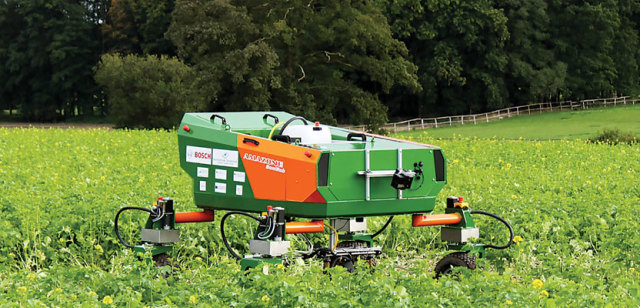
\includegraphics[width=\textwidth]{figuras/estado del arte/bonirob.jpg}
    \caption{Fotografía del robot \textit{BoniRob} \cite{Pittman2021}}
    \label{fig:bonirob}
\end{figure}

\subsection{Técnicas de localización}

La localización y clasificación de malas hierbas dentro del cultivo es uno de los grandes retos a los que se está enfrentando desde que se desea implementar este tipo de procesos \cite{Weis2008} dentro de la agricultura de precisión.

Este técnica se puede realizar de múltiples maneras, donde las más sencilla, es la propia inspección visual de forma manual, donde una persona experta va registrando la aparición de estas. Esta técnica resulta eficiente a la hora de localizar estas plantas, pero no es soportable para grandes cultivos, debido al enorme incremento de costes por el gran volumen de mano de obra necesaria. Debido a esto por lo que actualmente se tratan de desarrollar técnicas automatizadas para la realización de este tipo de tareas.

Algunas de las técnicas más desarrolladas a día de hoy se basan en el uso de cámaras hiper-espectrales \cite{Li2021} que funcionan recopilando información en todo el espectro electromagnético, pudiendo observar espectros de la luz no visible, consiguiendo recopilar gran cantidad de información de gran valor para poder diferenciar fácilmente entre diferentes tipos de vegetaciones. En la Figura \ref{fig:hyperespectral}, se puede observar un ejemplo de imagen tomada con este tipo de cámaras.

\begin{figure}[h]
    \centering
    \includegraphics[width=\textwidth]{figuras/estado del arte/hyperspectral_image.png}
    \caption{Comparación de fotografía tomada con cámara hiper-espectral y con cámara RGB \cite{igor_hyperspectral_2018}}
    \label{fig:hyperespectral}
\end{figure}

A pesar de esto, en los últimos años se ha visto fuertemente desarrollado el uso de cámaras RGB, que tan sólo son capaces de ver el espectro visible de la luz, las cuales usadas junto a técnicas de segmentación y clasificación de imágenes, son capaces de diferenciar de igual manera y con gran precisión los diferentes tipos de vegetación existentes. Estas tienen la problemática de que se ven muy influenciadas por la iluminación de la escena \cite{Lameski2017}, pero por otro lado, su precio es bastante inferior a las cámaras hiper-espectrales presentadas anteriormente \cite{Gasparovic2020}, por lo que resulta altamente interesante su uso en este tipo de aplicaciones.

\section{Clasificación de Imágenes}

En los últimos años, el desarrollo de la visión por computador ha sido un hito importante en el avance del despliegue de aplicaciones de robótica y automática, de manera que sea posible comprender el entorno que nos rodea extrayendo datos relevantes de las imágenes de forma automatizada.

Uno de los bloques más relevantes dentro de este, es el desarrollo de algoritmos de clasificación de imágenes, el cual se encarga de etiquetar imágenes en función del contenido que existe en ella, extrayendo propiedades que los hagan distinguibles de otras.

Desde un punto de vista clásico, esto se ha ido realizando siguiendo una serie de pasos determinados que son: el tratamiento de la imagen, la extracción de características y la clasificación. Todos estos pasos dependían del diseñador del algoritmo y del problema que se trataba de solucionar. Es por ello que muchos de estos algoritmos se centraban en la clasificación de cierto tipo imágenes en problemas cerrados y en el que tan solo ciertas condiciones eran contempladas.

Sin embargo, el avance de la tecnología ha visto un gran crecimiento en los desarrollos de algoritmos desde punto de vista de la computación basada en biología. Estos han entrado fuertemente en el ámbito del \textit{Machine Learning} (ML). Dentro de este campo, nacen las llamadas Redes Neuronales Convolucionales (CNN) \cite{Alzubaidi2021}, que se basan en el funcionamiento del cortex visual en los mamíferos. Estas son capaces de sintetizar todos los pasos que debían diseñarse manualmente desde el punto de vista de creación de los algoritmos de clasificación de imágenes. Además, son muy flexibles a la hora de reutilizar su arquitectura para la resolución numerosos problemas de clasificación de imágenes diferentes, que a priori no se parecen entre ellos, y que con otras técnicas, se tendría que haber modificado de forma importante la estructura del algoritmo.

\subsection{Redes Neuronales Convoluciones}

Las llamadas Redes Neuronales Convolucionales \cite{Alzubaidi2021}, han resultado una gran revolución dentro del campo de la clasificación de imágenes. A pesar de existir desde los años 80 \cite{Fukushima1980}, no ha sido hasta en los últimos 10 años cuando han cogido gran protagonismo debido al rápido crecimiento de la capacidad computacional de los ordenadores. Esto se ha debido sobretodo del desarrollo de las GPUs, las cuáles han permitido la paralelización del entrenamiento de estas redes.

Estas han tomado gran protagonismo en el campo desde que se impusieron a otros algoritmos clásicos en el desafío anual ILSVRC (\textit{ImageNet Large Scale Visual Recognition}), donde desde 2012, han sido este tipo de algoritmos los ganadores año tras año. Esto indica la gran capacidad de clasificación que tienen y su gran potencial.

En los últimos años, la forma clásica de usar estas redes es tomando redes pre-entrenadas con grandes conjuntos de datos clasificados y etiquetados, donde posteriormente, se re-entrenan con el \textit{dataset} objetivo. Esto es así, ya que necesitan gran cantidad de datos para este entrenamiento y no siempre se dispone de estas cantidades tan grandes de datos clasificados del problema objetivo.

Aún así, estas tienen numerosos inconvenientes que son necesarios conocer. En primer lugar, un grave problema es la gran potencia computacional necesaria para entrenar este tipo de algoritmos. Dependiendo del problema, en una infraestructura debidamente preparada computacionalmente para este tipo de tareas, el entrenamiento de una arquitectura clásica puede llevar desde días hasta semanas.

Estas grandes necesidades computacionales, pueden ser en ocasiones bastantes limitadoras, ya que hay veces se requiere que sean ejecutadas en pequeños ordenadores con capacidad computacional limitada para aplicaciones, por ejemplo, de agricultura de precisión como la que se han visto en apartados anteriores. Debido al gran requerimiento computacional que necesitan algunos tipos de redes de gran tamaño, esto lo hace actualmente inviable en muchos casos.

Otro problema que se ha localizado, es como las arquitecturas más empleadas en la actualidad tienen un carácter generalista, no adaptándose de forma adecuada al problema que se está tratando de resolver. Esto lleva a generar cierto interés a generar nuevas arquitecturas que se adapten de forma más adecuada al problema en cuestión.

Por último, redes de gran tamaño y generales, necesitan además de gran cantidad de datos etiquetados y balanceados para ser empleado en la fase de entrenamiento de las mismas \cite{Alzubaidi2021}, lo que resulta en muchos de los casos, una tarea farragosa y muy costosa económicamente. Ya no solo la gran duración de los entrenamientos, sino la gran cantidad de tiempo y recursos que son necesarios para generar estas grandes librerías de datos clasificadas para ciertas aplicaciones. 

Ya se han intentado poner soluciones a este tipo de problemas, empleando pequeños conjuntos de datos para generar arquitecturas que se adapten de manera adecuada a este tipo de entradas \cite{zoph2018learning}, de forma relativamente sencilla.

Es por estas desventajas anteriormente comentadas, por lo que se cree necesario la búsqueda de una solución para encontrar redes de menor tamaño y más fácilmente entrenables. Esto llevará a que estas puedan ser ejecutadas en máquinas de menor potencia y capacidad, de manera que tampoco se requiera una cantidad demasiado grande de datos clasificados para que funcionen de manera satisfactoria. Esto, finalmente llevara a conseguir arquitecturas de CNNs más optimizadas al \textit{dataset} que se está empleando, consiguiendo de esta manera mejores resultados.

Para esto se propone el uso de algoritmos de optimización, de tal manera, que se diseñen nuevas arquitecturas de CNNs, que en el caso de este trabajo, clasifiquen de manera sencilla y rápida, diferentes tipos de malas hierbas para su tratamiento posterior con técnicas de Agricultura de Precisión. 

Se proponen, en la actualidad, diferentes metodologías para encontrar este tipo de redes, aunque en el último año, se ha visto la aparición del uso de Algoritmos Genéticos para estos mismos propósitos \cite{Sun_2020}. Los Algoritmos Genéticos son técnicas de optimización bio-inspiradas, basadas en la teoría clásica de la evolución, donde numerosas soluciones tratan de competir por los recursos existentes. Aún son pocos los trabajos que se encuentran en este ámbito, pero los resultados que se obtienen son prometedores.

A partir de esto, se crea la hipótesis que se tratará de verificar durante el desarrollo de este trabajo. Esta hipótesis establece que, empleando Algoritmos Genéticos, se pueden generar arquitecturas de CNNs de menor tamaño, más fácilmente entrenables y con mejor desempeño que las empleadas en la actualidad para propósitos de detección y clasificación de malas hierbas en aplicaciones de agricultura de precisión.
  % INCLUDE: estado del arte
% !TEX root = ../my-thesis.tex
%
\chapter{DESARROLLO TEÓRICO}
\label{sec:desarrollo teórico}

A lo largo de este capítulo, se desarrollara la teoría básica necesaria para la comprensión y desarrollo de este trabajo. Es por ello que será necesaria la explicación del funcionamiento de los Algoritmos Evolutivos, los Algoritmos Genéticos y de los parámetros que entran en juego dentro del mismo. De la misma manera, se realizará una introducción a la implementación de Redes Neuronales y más específicamente, a las Redes Neuronales Convolucionales, que serán el resultado final del trabajo.

\section{Algoritmos Evolutivos}

Los Algoritmos Evolutivos abarcan la resolución de problemas de optimización o búsquedas de soluciones dentro del ámbito de los algoritmos bio-inspirados \cite{10.5555/2432058}. Esto quiere decir que se basan en emplear analogías con sistemas naturales o sociales para el diseño de métodos heurísticos no deterministas.

Estos algoritmos además forman parte de una de las ramas de la inteligencia artificial. Básicamente su uso está bastante extendido en la resolución de problemas con espacios de búsquedas grandes y no lineales, donde otros métodos encuentran gran dificultad en encontrar alguna solución en un tiempo razonable.

En el uso de esto algoritmos se realizan a partir de una \textbf{población} de individuos, los cuales son posibles candidatos a solución de un problema. Esta se verá alterada tras una serie de procesos que nos llevará a encontrar mejores individuos o soluciones. Cada ciclo de transformación equivale a una \textbf{generación}. Después de cierto número de generaciones, se espera que los mejores individuos de esta población se localicen de forma bastante próxima a la solución esperada del problema.

Cada uno de los individuos de la población ha de ir codificado de tal manera que esta se vaya transmitiendo de generación en generación. Esta codificación también es conocida como \textbf{genotipo} y es la principal diferencia que existe entre los diferentes tipos de algoritmos evolutivos como veremos posteriormente. Este genotipo está formado por \textbf{genes} que es la pieza básica de información que codifica a nuestro individuo. Todos estos no pueden ser interpretados directamente, por lo que se necesita que a partir de esta codificación se forme la forma analizable del individuo.

A partir del genotipo, se han de formar los rasgos visibles del individuo, también conocido como \textbf{fenotipo}. Este es la representación directa de la información genética. Pueden darse casos en la que la codificación genética no siempre pueda formar una correspondencia directa en el fenotipo y que se deban dar unas condiciones determinadas, en las siguientes generaciones, para que cierta información genética se vea definitivamente representada en el individuo.

Como se puede ver, usando este tipo de algoritmos se combinan técnicas de búsqueda aleatoria, que viene dada por la transformación de la población, y búsqueda dirigida, dada por la selección de los individuos. Con esto se consigue abarcar un gran espacio de búsqueda, en relativamente poco tiempo, en comparación a otros algoritmos de optimización de problemas.

\subsection{Funcionamiento general}

Todos los algoritmos evolutivos tienen la similitud de que comparten un mismo esquema de funcionamiento. Estos vienen heredados de la teoría clásica de la evolución y emplean mecanismos evolutivos naturales como la reproducción, la mutación y la selección natural \cite{10.5555/2432058}.

\begin{figure}[h]
    \centering
    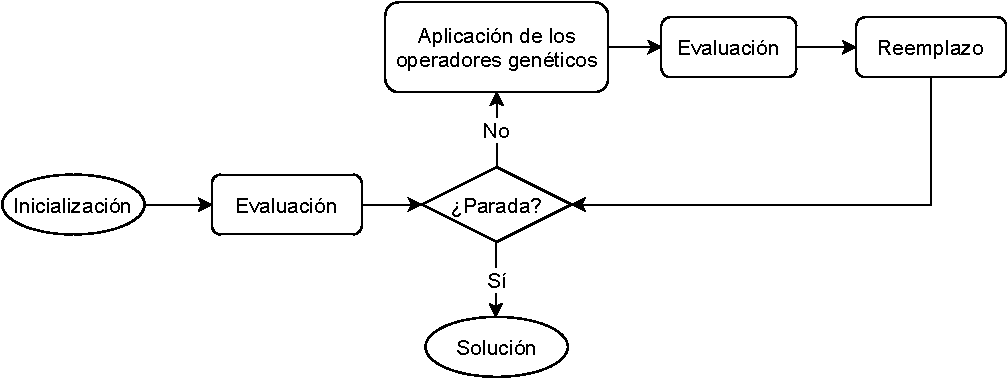
\includegraphics[width=\textwidth]{figuras/desarrollo teorico/Algoritmo_Evolutivo.pdf}
    \caption{Esquema de funcionamiento genérico de los Algoritmos Evolutivos}
    \label{fig:diagrama_alg_evolutivo}
\end{figure}

En la figura \ref{fig:diagrama_alg_evolutivo}, se describe el funcionamiento de un algoritmo evolutivo genérico. En él, se pueden ver las diferentes etapas por las que debe ir transitando cada uno de estos algoritmos.

En primer lugar, en la etapa de \textbf{inicialización} se crea una población del tamaño deseado, la cual esta compuesta por individuos que codifican diferentes soluciones muestreadas aleatoriamente dentro del espacio de búsqueda del problema. 

Como se veía anteriormente, cada individuo codifica una solución al problema propuesto y los operadores trabajan sobre esta codificación y no sobre las soluciones. Es por ello que es necesario posteriormente una etapa de \textbf{evaluación} donde se decodifica a este individuo y se obtiene la solución que representar para evaluar la calidad de este.

Si algunos de los individuos cumple los criterios dados para la solución del problema, se termina el algoritmo y se devuelven las mejores soluciones. De no ser así, se comienza un proceso iterativo en el cual se aplican diferentes \textbf{Operadores Genéticos} basados en los mecanismos evolutivos naturales para obtener nuevas soluciones que reemplacen a las antiguas. A cada iteración se la denomina \textbf{generación}.

Posteriormente, se debe volver a \textbf{evaluar} a todas las nuevas soluciones tal y como realizábamos anteriormente. Esto simula el desempeño de las tareas más importantes para la supervivencia de un individuo.

Una vez conocido el desempeño de las diferentes soluciones, se debe proceder a generar la población de la siguiente generación. Esto se realiza mediante la operación de \textbf{reemplazo}. Esto es debido a que se toma una población constante que simula un medio con recursos finitos, en los que los individuos deben competir entre ellos por la supervivencia dentro del grupo. En este paso es importante mantener la diversidad genética dentro de la población, por lo que se proponen técnicas donde todos los individuos tienen cierta probabilidad de sobrevivir asociado a su desempeño.

Tras esto, se debe verificar la \textbf{condición de parada} nuevamente, para determinar si se debe continuar con la ejecución del algoritmo o se debe proceder a salir del proceso iterativo. Se espera que con cada iteración el desempeño medio de la población vaya incrementándose hasta su convergencia en un óptimo o una solución definitiva.


\subsection{Clasificación de Algoritmos Evolutivos}

Como ya se veía anteriormente, existen numerosas técnicas de replicar el comportamiento evolutivo de los seres vivos en diferentes tipos de algoritmos. Esta división viene dada básicamente por la forma que toma el genotipo o codificación de los diferentes individuos de la población.

Esto alterará de forma inmediata la forma en la que los diferentes genotipos realizan las diferentes operaciones de mutación y cruce, por lo que se tienen que definir nuevos operadores para cada uno de estos tipos de algoritmos evolutivos.

Existen tres aproximaciones principales para estos mecanismos: los algoritmos genéticos, las estrategias evolutivas y la programación genética.

Los \textbf{Algoritmos Genéticos} \cite{Holland1984} emplean una codificación binaria, por lo que cada gen del genotipo esta formado por un valor ``0'' o ``1'' según corresponda. En la figura \ref{fig:ej_AG} podemos ver un ejemplo de esta representación.

Por otro lado, las \textbf{Estrategias Evolutivas} \cite{Beyer2002} se diferencian de las anteriores que la codificación se basa en el uso de número naturales que pueden ser representados de forma continua o discreta, según el problema. En la figura \ref{fig:ej_EE} podemos ver un ejemplo de esta representación.

Por último, en la \textbf{Programación Genética} \cite{koza1992genetic} la representación de los individuos es bastante diferente a los anteriores, y es que se emplean estructuras de arboles. En ella cada nodo del árbol expresa una función como operador y cada terminal del nodo, por el contrario, contiene un operando, por lo que se pueden generar expresiones de manera bastante sencilla. En la figura \ref{fig:ej_PG} podemos ver un ejemplo de esta representación.

\begin{figure}[h!]
\centering
    \begin{subfigure}{0.51\textwidth}
        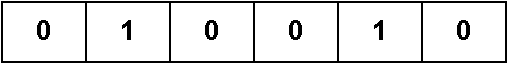
\includegraphics[width=\textwidth]{figuras/desarrollo teorico/Algoritmo_Evolutivo-ej_AE.pdf} 
        \caption{Algoritmo Genético}
        \label{fig:ej_AG}
    \end{subfigure}
    \begin{subfigure}{0.51\textwidth}
        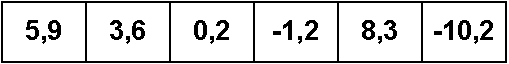
\includegraphics[width=\textwidth]{figuras/desarrollo teorico/Algoritmo_Evolutivo-ej_EE.pdf}
        \caption{Estrategias Evolutivas}
        \label{fig:ej_EE}
    \end{subfigure}
    \begin{subfigure}{0.65\textwidth}
        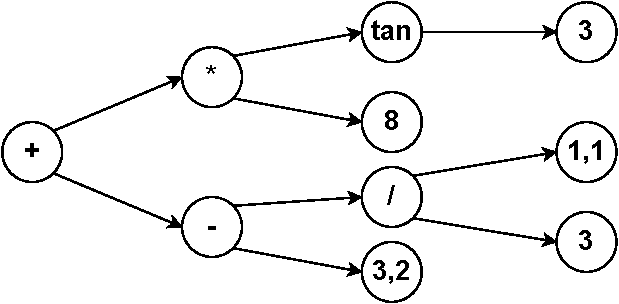
\includegraphics[width=\textwidth]{figuras/desarrollo teorico/Algoritmo_Evolutivo-ej_PG.pdf}
        \caption{Programación genética}
        \label{fig:ej_PG}
    \end{subfigure}
\caption{Ejemplos de representación de los diferentes tipos de Algoritmos Evolutivos}
\label{fig:ej_AE}
\end{figure}

\section{Algoritmos genéticos}

Los Algoritmos Genéticos vienen establecidos por Holland desde el año 1975 \cite{Holland1984} y posteriormente descritos de forma precisa en numerosos libros y artículos \cite{GoldbergDavidE.DavidEdward1989Gais}. En estos se demuestra como se trata de una técnica robusta y como puede solucionar con bastante éxito una amplia variedad de problemas a resolver de diferentes áreas.

Cabe destacar también, que este tipo de algoritmos cuentan con bastantes debilidades al no garantizar, por ejemplo, la localización de una solución óptima al problema a resolver. A pesar de esto, se demuestra empíricamente que el nivel de calidad de las soluciones es más que aceptable, y sobretodo, realizándolo en un tiempo competitivo con respecto a otras técnicas más especializadas de resolución de ciertos problemas.

Como ya se ha visto anteriormente, los Algoritmos Genéticos vienen dados por una codificación binaria del genotipo, lo que establece una forma de operar determinada, que lo diferencia del resto de Algoritmos Evolutivos.

En algunos problemas, puede que se tenga la necesidad que pequeños cambios en el genotipo resulten en pequeños cambios en el fenotipo, por lo que se puede acudir a codificaciones como la de Gray.

En las próximas páginas, se irá mostrando el funcionamiento y los parámetros que forman parte de este tipo de algoritmos y que son necesarios conocer, para la resolución posterior de forma adecuada de un problema determinado.

\subsection{Funcionamiento general}

El funcionamiento general de los Algoritmos Genéticos, se basan en lo ya visto en el funcionamiento general de los Algoritmos Evolutivos.

\begin{figure}[h]
    \centering
    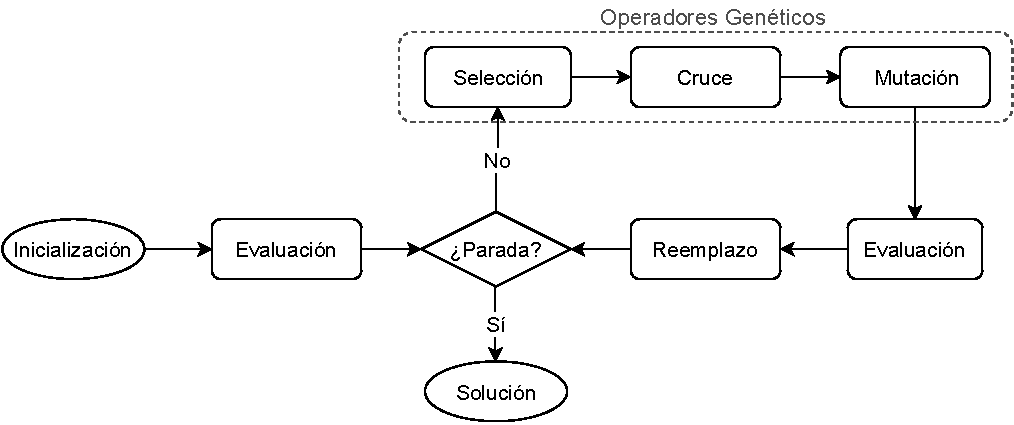
\includegraphics[width=\textwidth]{figuras/desarrollo teorico/Esquema_algoritmo_genetico.pdf}
    \caption{Esquema de funcionamiento de Algoritmos Genético Simple}
    \label{fig:diagrama_alg_genetico}
\end{figure}

En la figura \ref{fig:diagrama_alg_genetico}, se puede observar como se muestran los tres operadores genéticos que serán necesarios para la generación de nuevos individuos que serán candidatos a reemplazar generacionalmente a la anterior población.

Estos tres operadores son la \textbf{selección}, donde se deben seleccionar a los padres para la reproducción, el \textbf{cruce} donde con cierta probabilidad los padres generaran a los hijos y finalmente la \textbf{mutación}, donde nuevamente con cierta probabilidad aplicará una alteración en el genotipo en los hijos.

\subsection{Selección}

La selección de los padres es una operación que ha de realizarse de forma aleatoria, implementado diferentes técnicas para favorecer que los mejores individuos de una población a ser elegidos para posteriormente realizar el cruce con otro padre seleccionado.

Es importante en este paso garantizar que los mejores individuos de la población tengan mayor probabilidad de reproducirse frente a otros menos buenos. Aún así, hay que tener la cautela de dar oportunidad de selección a individuos menos buenos, ya que estos pueden portar en su genotipo partes útiles para el proceso de reproducción.

Existen diferentes estrategias de selección que pueden ser seguidas en función del problema que se esté tratando de resolver. Entre ellas encontramos la selección por torneo, el ranking lineal, la selección aleatoria, el emparejamiento variado inverso y la selección por ruleta.

\begin{itemize}
    \item La \textbf{Selección por Torneo} (TS) es una de las estrategias más empleadas. En ella, la selección se basa en la generación de diferentes ``torneos'' o grupos de individuos escogidos al azar de la población. En estos se selecciona al mejor individuo entre ellos. La manera en el que se seleccionan los individuos se ajusta en función a la cantidad de participantes en el torneo. A mayor cantidad de individuos en un torneo, menor probabilidad de seleccionar a individuos menos buenos.
    
    \item En el \textbf{Ranking Lineal} (LR), la población se ordena en función de lo bueno que es el cada uno de los individuos. Esto se asocia a una probabilidad de selección de cada uno de los individuos en función de la posición que tomen cada uno de ellos. De esta manera se le da mayor probabilidad de selección a los mejores individuos.
    
    \item En la \textbf{Selección Aleatoria} (RS), como su nombre indica, se seleccionan a los individuos de forma azarosa. Esto quiere decir que no se mira que tan bueno es el individuo para seleccionarlo como padre.
    
    \item El \textbf{Emparejamiento Variado Inverso} (NAM), es un método que trata de buscar una selección de padres con carga genética diferente y evitar que dos individuos muy parecidos se reproduzcan después. Esto lo realiza mediante la selección de un padre aleatoria. Posteriormente se seleccionan un número N de padres y se escoge entre ellos el cual contenga más diferencias en el genotipo con el primer padre seleccionado.
    
    \item La \textbf{Selección por Ruleta} es el método más empleado para la selección de padres dentro de los Algoritmos Genéticos. En este se asigna una probabilidad de selección proporcional a la calidad del individuo y se selecciona a uno aleatoriamente.
    
\end{itemize}

La selección de una u otra estrategia de selección dependerá de las necesidades del problema a optimizar.


\subsection{Cruce}

El cruce los padres se asocia a la fase reproductiva de los individuos de la población en la cual se han de mezclar la información genética de los individuos seleccionados. Esto dará como lugar la creación de nuevos individuos que representarán los candidatos a individuos de la siguiente generación.

El cruce se realiza como forma de exploración guiada cerca de las soluciones conocidas, tratando de buscar los mejores genes en una zona local.

Para la realización de este cruce, se asocia a él una probabilidad por la cual establece cuando una pareja de padres generará o no descendencia. Normalmente se suelen seleccionar valores altos de probabilidad, entre el 0,6 y el 0,9 aproximadamente. Esto dependerá del problema que se esté tratando a resolver.

Además se piden más aspectos a tener en cuenta para la realización de este cruce, y es que los hijos deben heredar algunas de las características de cada uno de los padres. También, el resultado debe ser un genotipo válido y que conserve la forma definida dentro del problema. Destacar además que los genotipos creados deben ser capaces de generar, de la manera que se ha definido, fenotipos válidos para la resolución del problema.

Existen diferentes estrategias a seguir para la realización de este cruce, entre las que encontramos: el cruce en un punto, el cruce en N puntos y el cruce uniforme.

\begin{itemize}
    \item El \textbf{Cruce en un punto} (\textit{1-point Crossover}) se basa en la selección de un punto de cruce aleatorio dentro del genotipo de ambos padres. Los padres se dividen a partir de ese punto y se crean hijos intercambiando partes de los genotipos. Es por ello que el resultado de aplicar este son dos hijos con información genética de ambos padres.
    
    En la Figura \ref{fig:cruce_1_punto}, se puede ver un ejemplo de esta operación.\\
    
    \begin{figure}[h]
         \centering
         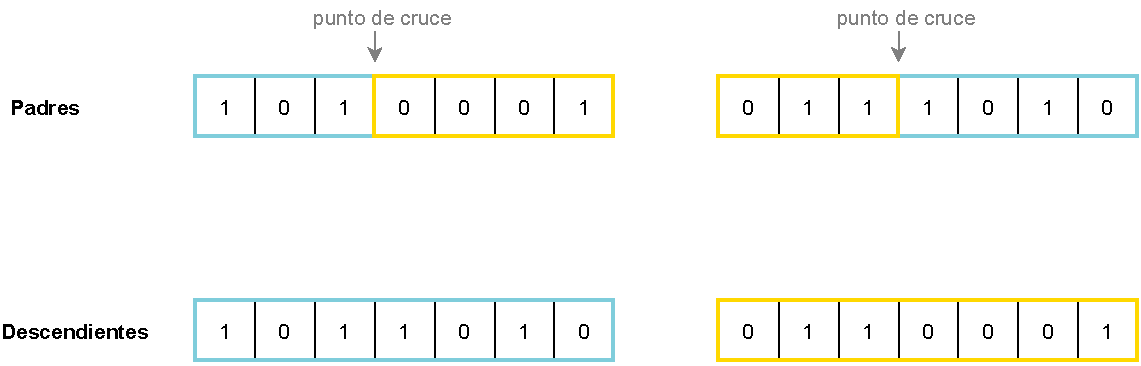
\includegraphics[width=1.1\textwidth]{figuras/desarrollo teorico/cruce_1_punto.pdf}
         \caption{Ejemplo de cruce en un punto}
         \label{fig:cruce_1_punto}
    \end{figure}
    
    Hay que tener diferentes cosas en cuenta, como que depende del orden en el que van apareciendo los genes y por lo tanto guarda un sesgo posicional, que depende del problema a resolver, este puede ser beneficioso o perjudicial.
    
    \item El \textbf{Cruce en N puntos} (\textit{N-point Crossover}) es una generalización del cruce en un punto anteriormente comentado. En este en vez de seleccionar tan solo un punto de corte, se seleccionan N puntos. Esto ayuda a que se fragmente de mayor medida la información genética de ambos padres.
    
    En la Figura \ref{fig:cruce_N_puntos}, se puede ver un ejemplo de la aplicación de esta operación.\\
    
    \begin{figure}[h]
         \centering
         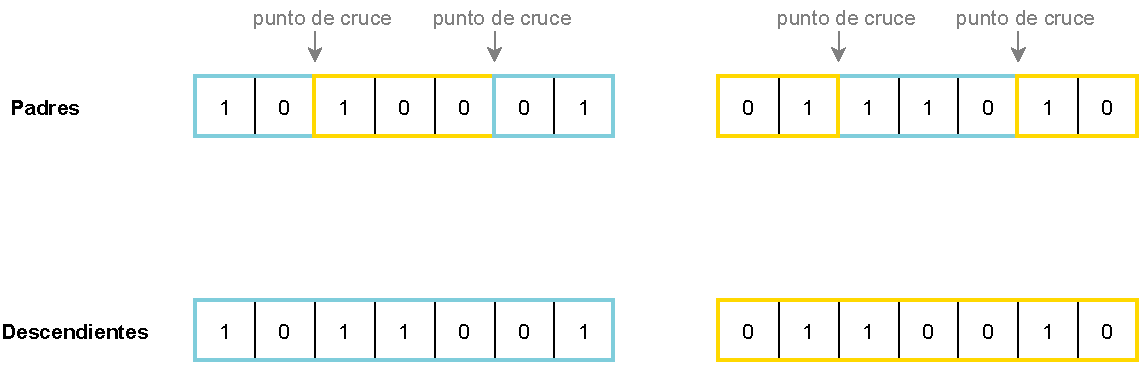
\includegraphics[width=1.1\textwidth]{figuras/desarrollo teorico/cruce_N_puntos.pdf}
         \caption{Ejemplo de cruce en dos puntos}
         \label{fig:cruce_N_puntos}
    \end{figure}
    
    \item Por último encontramos el \textbf{Cruce Uniforme} (\textit{Uniform Crossover}). En este la mezcla de información genética se realiza de forma aleatoria, en la cual se selecciona con cierta probabilidad por la que un determinado gen debe intercambiarse a lo largo del genotipo de ambos padres. En la Figura \ref{fig:cruce_uniforme}, se puede ver un ejemplo de la aplicación de esta operación.\\
    
    \begin{figure}[h]
         \centering
         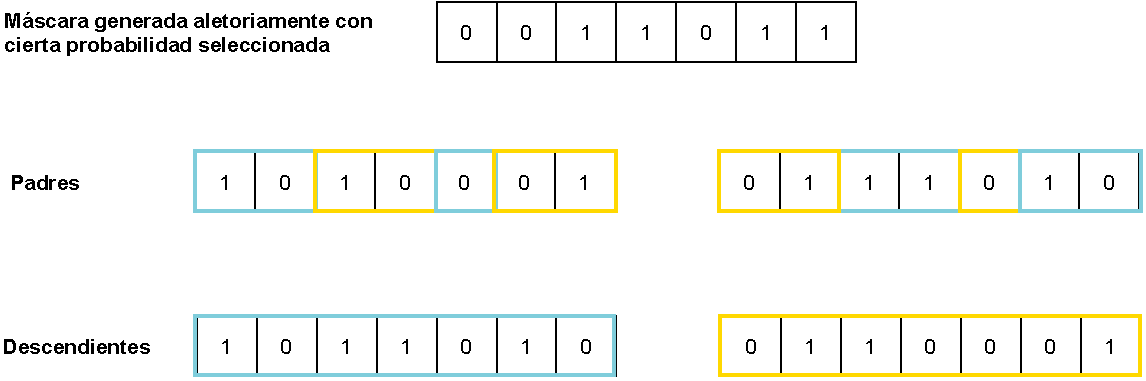
\includegraphics[width=1.1\textwidth]{figuras/desarrollo teorico/cruce_uniforme.pdf}
         \caption{Ejemplo de cruce uniforme}
         \label{fig:cruce_uniforme}
    \end{figure}

    En este tipo de cruce, la herencia del gen es independiente de su posición dentro del genotipo, por lo que se elimina el sesgo posicional que encontrábamos en las anteriores estrategias.

\end{itemize}


\subsection{Mutación}

La mutación es una operación que se realiza de forma individual a cada uno de los individuos de la población. Esto significa que se modifica el valor al azar de alguno de los genes del cromosoma de un individuo seleccionado de forma aleatoria dentro de nuestra población.

Esta operación es importante dentro del algoritmo, porque permite la exploración extensiva del espacio de búsqueda del problema, que solo con la operación de cruce no sería posible realizar. Esto es de vital importancia para asegurar la correcta convergencia del Algoritmo Genético.

La mutación es una operación bastante sencilla de implementar, ya que tan solo hay que definir una probabilidad por la que un individuo va a ser seleccionado para que mute. Esta probabilidad normalmente debe ser baja, para evitar convertir el algoritmo en un método de exploración aleatoria.

Posteriormente, tras tener el individuo seleccionado, se proporciona una nueva probabilidad a cada gen de su cromosoma para ser mutado, y en caso positivo, se cambia el valor de ese gen. El valor de este depende del problema a resolver.

En la Figura \ref{fig:mutacion}, se puede ver un ejemplo de esta operación.\\

\begin{figure}[h]
         \centering
         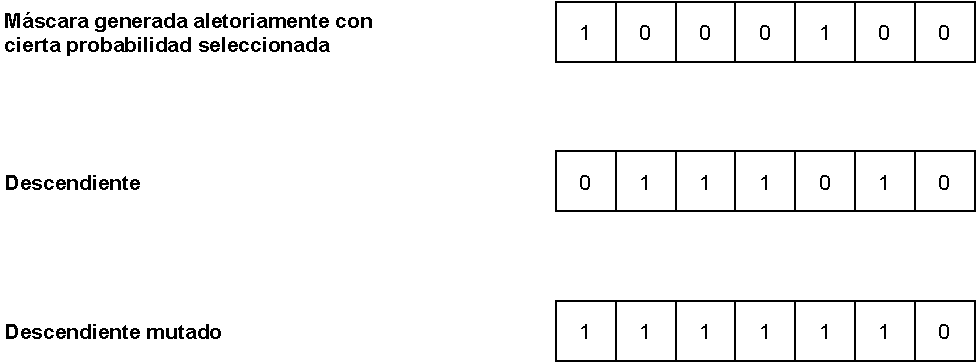
\includegraphics[width=\textwidth]{figuras/desarrollo teorico/mutacion.pdf}
         \caption{Ejemplo de operación de mutación}
         \label{fig:mutacion}
    \end{figure}

\subsection{Evaluación}

La evaluación es una de las fases más críticas dentro del algoritmos, ya que su definición de manera no adecuada, puede llevar a nuestro problema de optimización a no conseguir los resultados esperados.

En esta fase, se debe a partir del fenotipo del individuo, obtener un valor real el cual refleja el nivel de adaptación o desempeño que ha tenido este como solución a nuestro problema.

Esta evaluación se realiza normalmente a partir de una función objetivo o función \textit{fitness}. Esta vendrá dado por una expresión o por una métrica obtenida a partir del fenotipo del individuo en cuestión.

Esta nos interesa que cumpla cierta regularidad, por lo que dos individuos que se encuentren cercanos dentro del espacio de búsqueda, serán parecidos sus valores de \textit{fitness}.

Suele ser normal además, el establecer una penalización dentro de la propia función \textit{fitness}, debido a que puede haber zonas del espacio de búsqueda que no son deseadas o válidas, por lo que esto debe quedar reflejado en el desempeño de la solución encontrada.

\subsection{Reemplazo}

El reemplazo es el proceso por el cual se sustituyen a todos o a ciertos padres de la anterior población, por el resultado de las operaciones genéticas, a los que denominamos hijos.

Este proceso modela la limitación de recursos suficientes para todos los individuos de la población, por lo que se debe intentar mantener una población determinada o máxima.

Existen diferentes formas de plantear este proceso. Algunos vienen dados en función del número de hijos que sustituyen a cierto numero de padres. Estos modelos son: los Modelos Generacionales y Estacionarios.

\begin{itemize}
    \item El \textbf{Modelo Generacional} se caracteriza por que en cada generación, se crea un población totalmente nueva que sustituye íntegramente a la población anterior.
    \item El \textbf{Modelo Estacionario} donde los nuevos individuos reemplazan a uno o varios de los padres, pero no a todos. Es un modelo en el cual se trata de que los mejores individuos prosigan tras varias generaciones.
\end{itemize} 

Dentro de los Modelos Estacionarios encontramos diferentes estrategias para el reemplazo como son: Reemplazar al peor de la población, Torneo Restringido, Peor entre semejantes, y Algoritmo de Crowding Determinístico.

\subsection{Elitismo}

En ocasiones, se requiere la conservación de los mejores individuos a lo largo de las diferentes generaciones para que siga dando de su buena información genética a los nuevos individuos de la población.

Es por ello, que las medidas de selección en función de lo bueno que es el individuo pueden no asegurar siempre la supervivencia de estos dentro de la población, por lo que a veces es necesario asegurar su no desaparición de la población.

Para este problema se crea la estrategia denominada \textbf{Elitismo}, por la cual se protegen a los mejores individuos de una población ante los mecanismos de selección, cruce y mutación, conservándolos intactos en la siguiente generación.

Este mecanismo bajo ciertas condiciones generales, garantiza la convergencia en un óptimo global y además en la práctica ayuda a una mejora de la velocidad de obtención de buenos resultados.



\section{Redes Neuronales Artificiales}

Las Redes Neuronales Artificiales se engloban dentro de las técnicas de aprendizaje automático o aprendizaje máquina (\textit{Machine Learning}) como algoritmos bio-inspirados \cite{10.5555/523781}, al igual que se veía con los Algoritmos Evolutivos.

Estas técnicas, sin embargo, tratan de imitar el funcionamiento biológico simplificado de las neuronas que componen el cerebro. Al igual que el cerebro, la interconexión de gran cantidad de estas neuronas se tratan de emplear para la resolución de problemas como la memorización o la clasificación, entre otras.

Este Aprendizaje Automático donde se engloba este algoritmo, tiene como fin el desarrollo de sistemas que de forma autónoma y en base a la experiencia, sean capaces de cambiar su comportamiento, consiguiendo la capacidad de aprender a partir de unos datos dados. 

El aprendizaje automático se divide en dos tipos: el Aprendizaje Supervisado y el Aprendizaje No Supervisado. Las Redes Neuronales Artificiales forman parte del primer grupo, ya que los datos de entrada que recibe, van etiquetadas, de manera que es capaz de asociar el dato con la etiqueta correspondiente.

\subsection{Estructura y funcionamiento}

Para realizar la explicación del funcionamiento de las redes neuronales artificiales, se comenzará describiendo la red neuronal más simple existente. Esta está formada por una neurona y una única entrada \cite{10.5555/523781}. En la figura \ref{fig:neurona_simple}, se puede ver el esquema de esta red representada.

\begin{figure}[h]
    \centering
    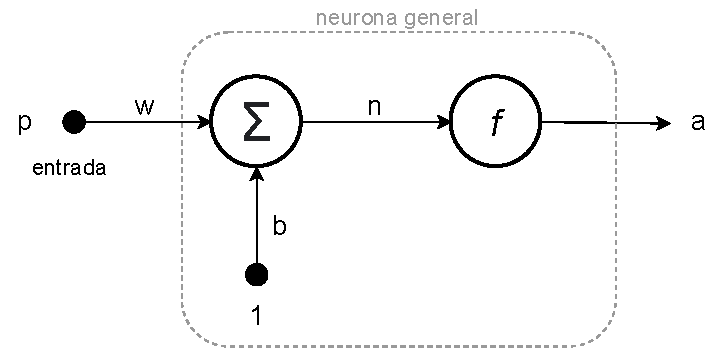
\includegraphics[width=0.7\textwidth]{figuras/desarrollo teorico/neurona.pdf}
    \caption{Esquema simple de una neurona artificial de una entrada y una salida}
    \label{fig:neurona_simple}
\end{figure}


El funcionamiento de esta es muy simple. En la entrada, se recibe un escala $p_1$ que es multiplicado por un peso $w_1$. Esto entra dentro de un sumatorio donde se entrarán además el resto de entradas en caso de tenerlas. Además, al sumatorio entra una señal de \textit{bias} representado por la letra $b$ en nuestro esquema. Por simplificación, esta señal se modela como una entrada siempre a 1 multiplicada por un valor $w_0$. A la salida del sumatorio, nos encontramos una función de transferencia $f$. A sus salida obtenemos por lo tanto la expresión \ref{eq:neurona_simple}.

\begin{equation}
    a = f(b + w_1 * p_1) = f(w_0 * 1 + w_1 * p_1)
    \label{eq:neurona_simple}
\end{equation}

De esta expresión, queda como parámetro de diseño la función de transferencia y como parámetros calculables las diferentes $w_i$. El primero es impuesto por el diseñador de la red, sin embargo, el segundo es un valor que es calculado mediante cierta regla de aprendizaje.

De este pequeño ejemplo, se puede deducir una expresión genérica para una neurona de $n$ entradas, quedando de la manera reflejada en la expresión \ref{eq:neurona_simple_n}

\begin{equation}
    a = f(\sum^{n}_{i=0} p_i w_i)
    \label{eq:neurona_simple_n}
\end{equation}

Una vez conocido el principio básico de funcionamiento de una neurona, la explicación de una red neuronal se basa en la interconexión de forma lógica de gran cantidad de estas neuronas. En función del problema que se intente resolver, la interconexión se realizará de diferentes maneras, formando numerosas topologías de neuronas en función de las necesidades de la red. Aún así, las redes neuronales suelen seguir un esquema bastante claro como el que se puede ver en la figura \ref{fig:red_neuronal}.

\begin{figure}[h]
    \centering
    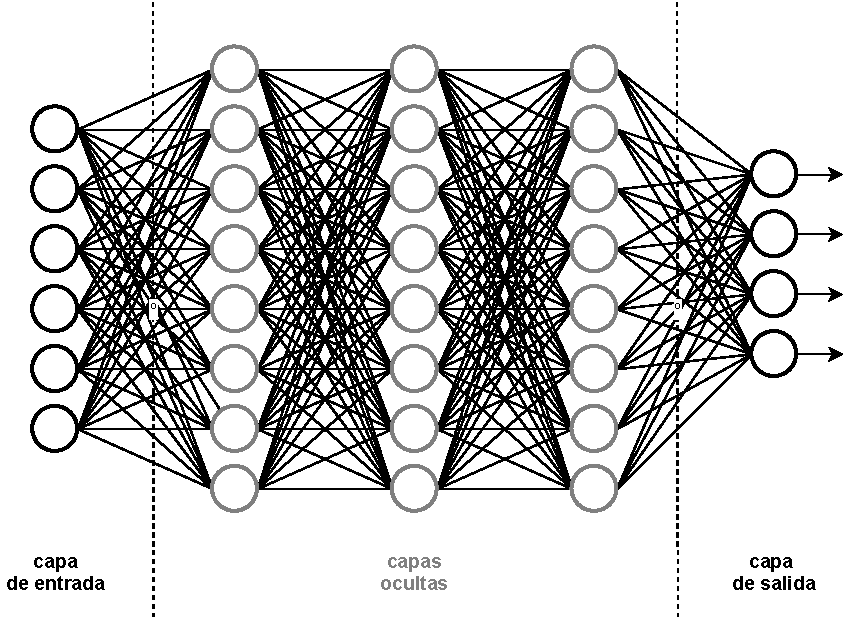
\includegraphics[width=1.1\textwidth]{figuras/desarrollo teorico/red_neuronal.pdf}
    \caption{Esquema de red neuronal artificial simple completamente conectada}
    \label{fig:red_neuronal}
\end{figure}

Como se puede ver, las neuronas se agrupan normalmente en capas de cierta profundidad, dada por el numero de neuronas en cada capa. Cada una de las capas, se interconectan totalmente entre ellas, obteniendo una topología de capas totalmente conectadas. Dentro de las capas se suele hablar de tres tipos:

\begin{itemize}
    \item \textbf{Capas de entrada}: En esta capa no existe procesamiento, ya que simplemente en estas se introducen los valores de entrada a la red. Esta tendrá tanta profundidad como datos de entrada se tengan.
    \item \textbf{Capas ocultas:} Estas capas no tienen interconexión directa con el entorno. El número de capas y su profundidad dependerán del problema que se quiera resolver.
    \item \textbf{Capas de salida:} Estas capas se corresponden con el final de nuestra red neuronal, y tendrá tanta profundidad como etiquetas o valores de salida se tengan.
\end{itemize}

\subsection{Función de Activación}

La función de transferencia comentada en el apartado anterior, se le denomina \textbf{Función de Activación}. Esta, como ya se comentó, su elección cae en función del criterio del diseñador de la red y del problema a resolver. Ahora se va a pasar a mostrar las funciones más empleadas en la actualidad.

\begin{itemize}
    \item \textbf{ReLU:} Esta función de activación sigue la expresión $a(x) = max(0,x)$. Como se puede observar se trata de una función bastante simple, ya que no requiere de ningún gran calculo, por lo que su uso está bastante extendido debido a su bajo coste computacional. Como desventaja, podemos ver que se trata de una expresión no derivable. En la figura \ref{fig:relu} se puede ver como es esta función.
    
    \begin{figure}[!ht]
    \centering
    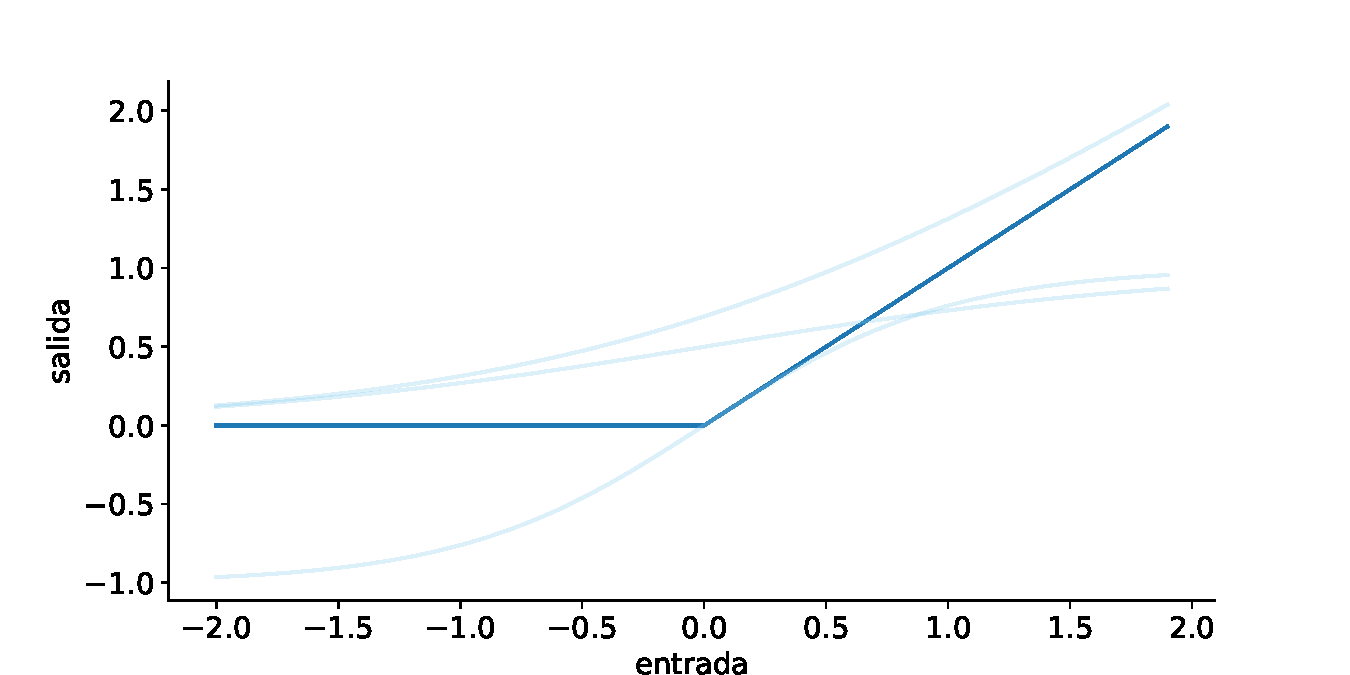
\includegraphics[width=\textwidth]{figuras/desarrollo teorico/relu.pdf}
    \caption{Representación de función de activación ReLU}
    \label{fig:relu}
    \end{figure}

    
    \item \textbf{Softplus:} Esta función de activación sigue la expresión $a(x) = log(1 + e^x)$. Como se puede observar, es una expresión bastante más compleja de resolver con respecto a la \textit{ReLU}, lo cuál se traduce en mayor coste computacional. Cómo ventaja frente a la anterior, es su derivabilidad, lo cuál lo hace adecuado para algoritmos de entrenamiento de la red que se verán posteriormente. En la figura \ref{fig:softplus} se puede ver como es esta función.
    
    \begin{figure}[!ht]
    \centering
    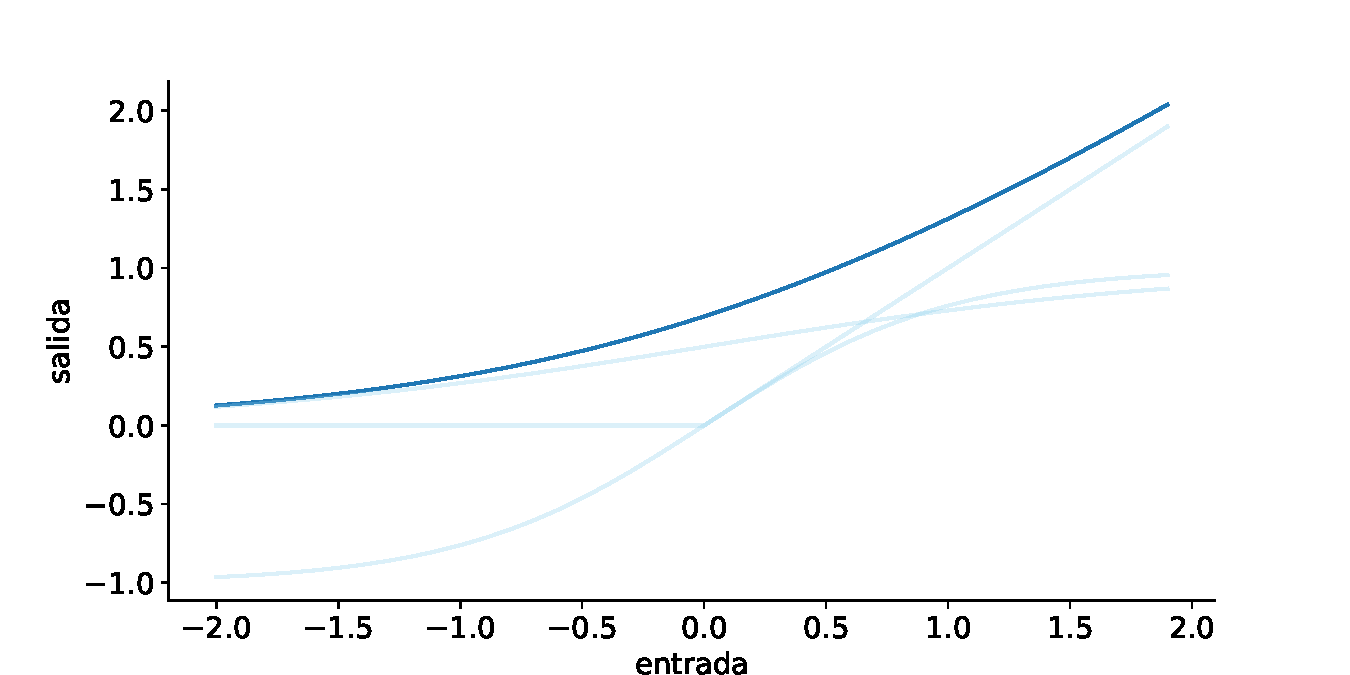
\includegraphics[width=\textwidth]{figuras/desarrollo teorico/softplus.pdf}
    \caption{Representación de función de activación Softplus}
    \label{fig:softplus}
    \end{figure}
    
    \item \textbf{Tangente hiperbólica (tanh):} Esta función de activación sigue la expresión $a(x) = tanh(x)$. Es también ampliamente usada, como la anterior, debido a su derivabilidad en todo su rango. En la figura \ref{fig:tanh} se puede ver como es esta función.
    
    \begin{figure}[!ht]
    \centering
    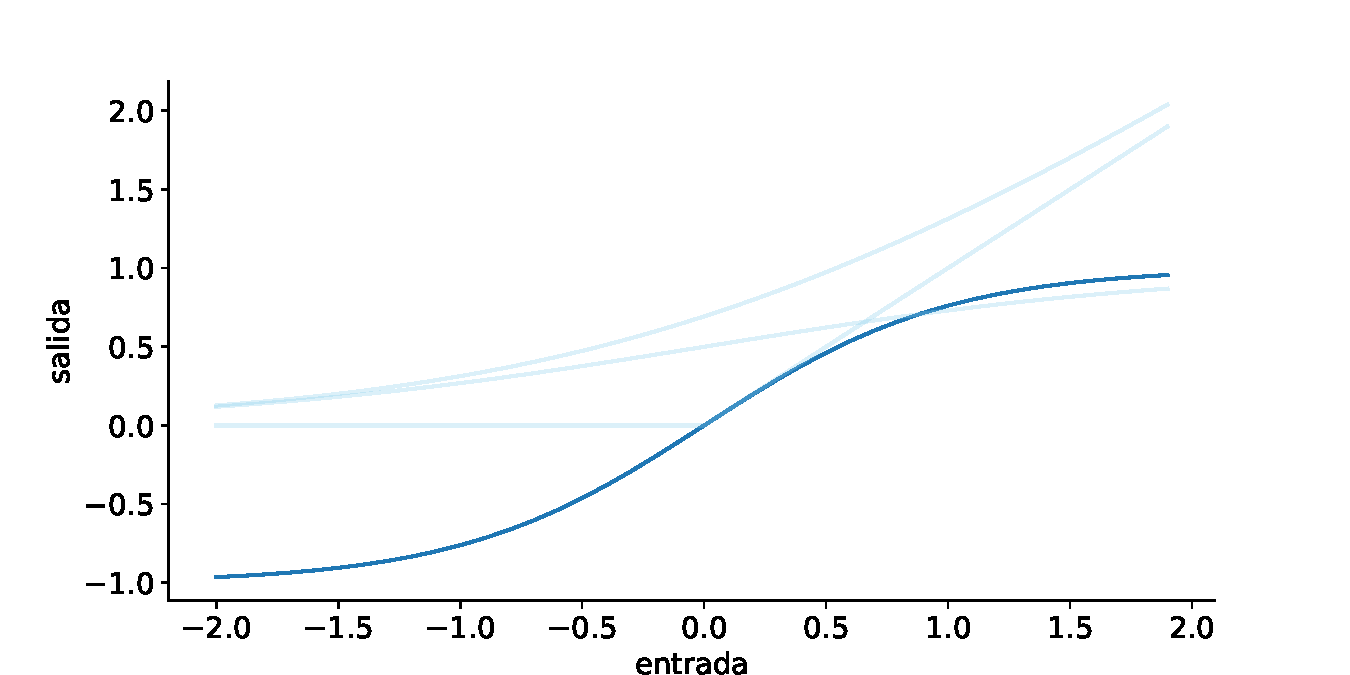
\includegraphics[width=\textwidth]{figuras/desarrollo teorico/tanh.pdf}
    \caption{Representación de función de activación tanh}
    \label{fig:tanh}
    \end{figure}
    
    \item \textbf{Sigmoide:} Esta función de activación sigue la expresión $a(x) = \frac{1}{1 + e^{-x}}$ y tiene una forma similar a la dada por la tangente hiperbólica. Comparte también que es derivable en todo su rango. En la figura \ref{fig:sigmoid} se puede ver como es esta función.
    
    \begin{figure}[!ht]
    \centering
    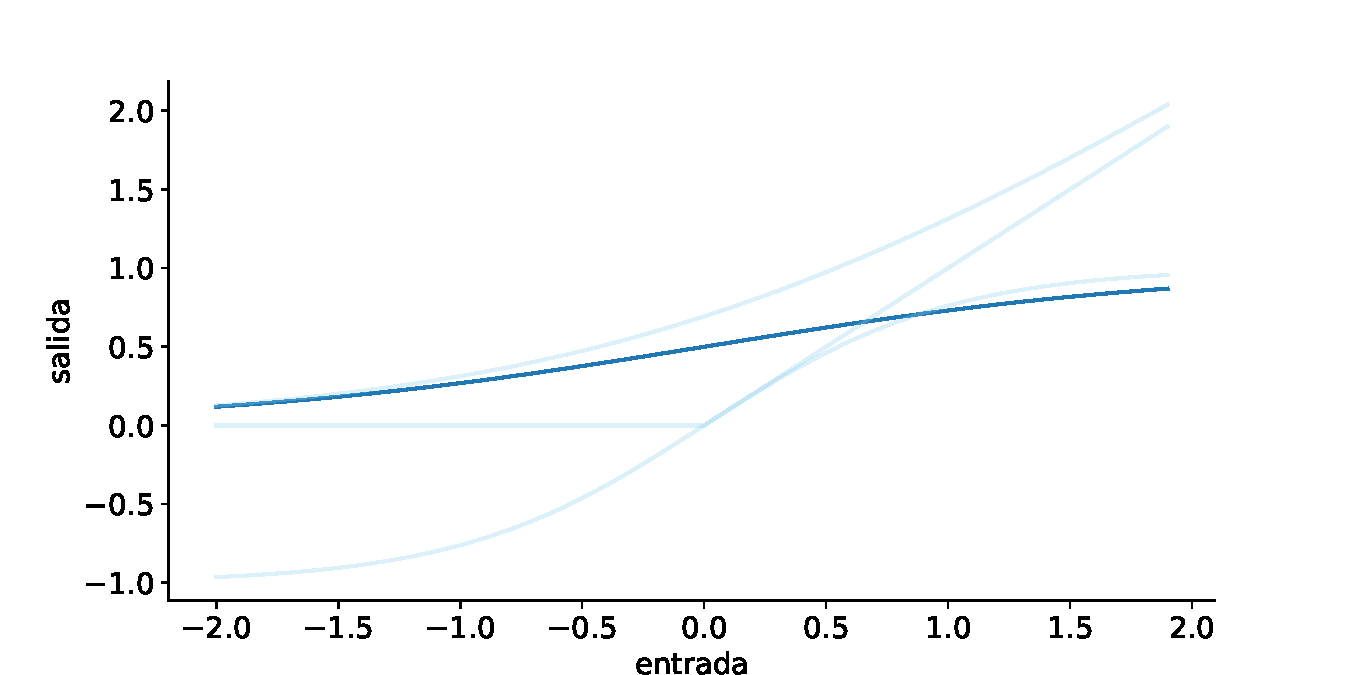
\includegraphics[width=\textwidth]{figuras/desarrollo teorico/sigmoid.pdf}
    \caption{Representación de función de activación Sigmoide}
    \label{fig:sigmoid}
    \end{figure}
    
\end{itemize}



\subsection{Entrenamiento}

Una vez diseñada como va a ser la arquitectura de la red neuronal artificial hay que comenzar a enseñarle a resolver el problema propuesto. El entrenamiento es como se conoce al proceso de aprendizaje de las redes neuronales artificiales. Este básicamente se trata de un problema de optimización de la red \cite{Aggarwal2018_training}.

Para ello se realiza una base de datos, en los cuales se conoce tanto la entrada como la salida, del problema a solucionar. De este se toma una parte, la cual irá a esta etapa de entrenamiento. El resto se empleará para la validación posterior del modelo. Normalmente se emplean más cantidad de datos para el entrenamiento que para la validación.

Los datos de entrenamiento seleccionados, se irán pasando por la red generando una salida, la cuál se comparará con la salida real y se tratará de corregir ajustando los pesos $w_i$ anteriormente comentados.

Para ver la desviación entre la salida de la red y la salida solución del problema, se emplean diferentes cálculos del error, de los que se destacan el uso de: el Error Cuadrático Medio (ECM), el Error Medio Absoluto (EAM) y la Entropía Cruzada.

La fase de optimización de este problema, trata de conseguir que el error que se acaba de comentar llegue a tener valor nulo. Las opciones de resolver este problema son bastante diferentes, pero casi todas se basan en una relación proporcional entre la variación de los pesos y el error cometido. Uno de los algoritmos más empleados para la optimización de este problema es el \textbf{Descenso del Gradiente} el cuál viene dado por la expresión \ref{eq:desc_gradiente}.

\begin{equation}
    \Delta w(t+1)= -\gamma * \nabla E(w(t))
    \label{eq:desc_gradiente}
\end{equation}

siendo $\Delta w(t+1)$ la variación de los pesos en un tiempo $t$, $\gamma$ el ratio de aprendizaje o \textit{Learning Rate} y $E$ la función de error a minimizar.

En todos los método de optimización, existe un parámetro en común, que es el \textit{Learning Rate} (LR), el cual indica el tamaño del salto en cada una de las iteraciones. Existen diferentes optimizadores que lo varían en función del resultado en las iteraciones previas.

Es totalmente vital la buena elección del valor de LR, ya que un valor muy alto de este, puede hacer que nuestro problema nunca converja, haciendo que el entrenamiento sea inútil. Por otro lado, un asignación muy bajo, hará que nuestro aprendizaje sea excesivamente lento, aunque nos asegura la convergencia. Es por ello que es primordial encontrar un valor adecuado para la resolución del problema dado.

El proceso de optimización además va acompañado de otro algoritmo necesario a la hora de deducir el error cometido por cada una de las neuronas, y así ajustar sus pesos. Es se llama \textit{Backpropagation} \cite{Goodfellow-et-al-2016} y como su nombre indica, implica el calculo del error propagándolo desde la capa de salida hasta la capa de entrada a través del resto de capas ocultas.

\subsection{\textit{Overfitting}}

Durante el aprendizaje, es necesario conseguir un numero de iteraciones adecuado para resolver nuestro problema de optimización. Esto es debido a que no es adecuado siempre que se llegue a un error de optimización igual a nulo. Esto es así, debido a que en principio, se quiere que nuestra red sea capaz de generalizar y por lo tanto, sea capaz de resolver problemas no vistos dentro del conjunto de datos de entrenamiento.

Un entrenamiento excesivo de nuestra red puede hacer que se llegue a un caso de sobre-entrenamiento o \textit{overfitting} \cite{salman2019overfitting}. Esto quiere decir que nuestra red, tan solo es capaz de resolver de forma adecuada los valores entregados en el conjunto de datos de entrenamiento, sin embargo, no es capaz de hacerlo de forma correcta con los datos de validación.

Es por ello que tras cada cierto numero de iteraciones, sea adecuado observar como resuelve la red el problema con los datos de validación, para poder establecer un punto de parada de entrenamiento de la red. Esto se ve de forma muy descriptiva en la figura \ref{fig:overfitting}.

\begin{figure}[!h]
    \centering
    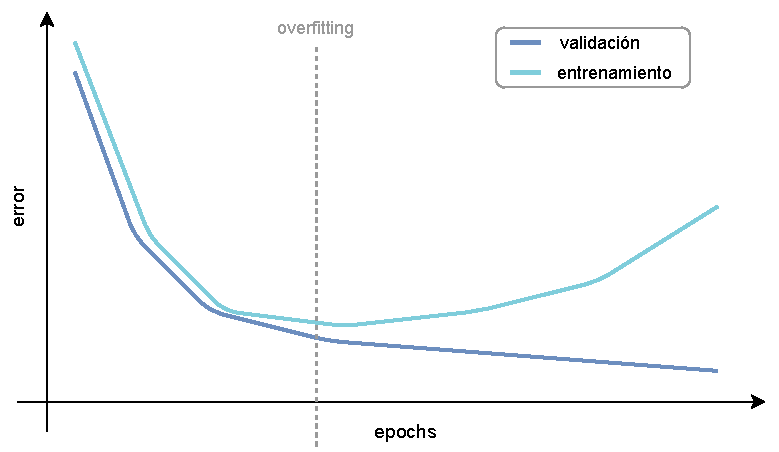
\includegraphics[width=1\textwidth]{figuras/desarrollo teorico/overfitting.pdf}
    \caption{Localización del \textit{overfitting} en un entrenamiento clásico}
    \label{fig:overfitting}
    \end{figure}

Existen diferentes tipos de entrenamiento que intentan paliar esta problemática. Estos son: el Entrenamiento estocástico y el Entrenamiento por lotes.

\begin{itemize}
    \item \textbf{Entrenamiento Estocástico} (\textit{Stochastic training}): En este tipo de entrenamiento se toman al azar de nuestro conjunto de datos, calculando su error y realizando los cambios de pesos correspondientes. Esta etapa (\textit{epoch}) habrá tantas iteraciones como datos.
    
    \item \textbf{Entrenamiento por lotes} (\textit{Batch training}): En este tipo de entrenamiento, los datos se clasifican en varios lotes aleatorios de un determinado tamaño de lote (\textit{Batch size}). En este se calcula el error a partir de la suma de los errores de cada una de las muestras de los diferentes datos. En este se consigue una mejor optimización porque se toman todos los datos de entrenamiento, pero es mas costoso cada \textit{epoch} computacionalmente hablando, ya que se necesitan muchos \textit{epochs} para la obtención de un resultado correcto.
\end{itemize}


\section{Redes Neuronales Convolucionales}

Una Red Neuronal Convolucional o \textit{Convolutional Neural Network} (CNN) es una estructura de red basada en redes neuronales. Este se encuentra dentro de la categoría de \textit{Deep Learning} debido al numero necesario de capas implicadas en este tipo de arquitecturas. Su principal diferencia con otro tipo de Redes Neuronales Artificiales es su capacidad de tomar una imagen como entrada y extraer diferentes sesgos o características de estas imágenes.

El diseño de estas redes se sigue asemejando al comportamiento de las neuronas de nuestro cerebro. En este caso inspirado en el comportamiento realizado por el córtex visual. Ambas trabajan tratando de deducir potenciales de acción de la imagen para tratar de sacar características de la misma. Esta es capaz de obtener dependencias espaciales y temporales de una imagen.

\subsection{Estructura}

Dentro de la arquitectura habitual de una CNN, existen diferentes tipos de capas esenciales que componen esta \cite{Aggarwal2018}. Cada una de ellas, se encarga de realizar unas operaciones determinadas dentro de la misma. Es por ello que para el correcto funcionamiento, es necesario conocer que actividades realiza dentro de la propia red.

En primer lugar, se debe hablar de las \textbf{Capas de Convolución}. Estas básicamente se basan en la aplicación de diferentes filtros o \textit{kernels}, que son modelados de la misma manera que son modelados los pesos dentro de una red neuronal convencional, de manera que son capaces de extraer características importantes de una imagen de entrada dada. A la salida de esta capa, encontramos los mapas de características o \textit{features maps}, los cuales son el resultado de aplicar la operación de convolución entre la imagen de entrada y el \textit{kernel}. En la figura \ref{fig:convolucion}, se puede ver un ejemplo de lo anteriormente comentado.\\

\begin{figure}[!h]
\centering
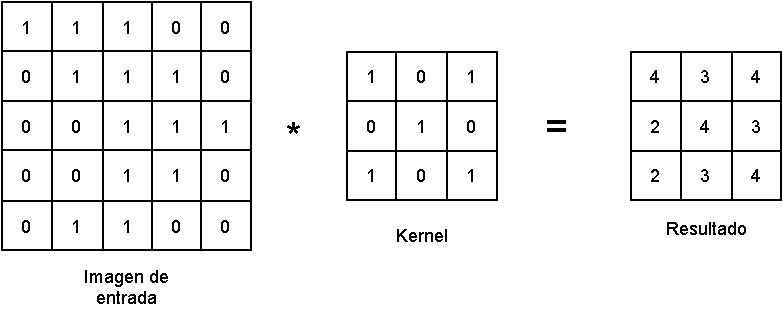
\includegraphics[width=0.9\textwidth]{figuras/desarrollo teorico/Convolucion.pdf}
\caption{Aplicación de convolución a imagen de entrada 5x5 con filtro 3x3 y \textit{stride} de 1}
\label{fig:convolucion}
\end{figure}

Las imágenes de entrada suelen tener dos dimensiones espaciales y tres canales, una por color. Es por esto que los \textit{kernel}, al aplicarse en imágenes en dos dimensiones, suelan tener de igual manera dos dimensiones. Su tamaño es variable y depende por tanto del diseñador de la arquitectura establecer un tamaño para estos, en función de las necesidades del problema a resolver. El número de \textit{kernels} que se emplean por capa también son un producto del diseñador de la arquitectura de la red y deben ser definidos al principio. A mayor cantidad de \textit{kernels}, más cantidad de características serán capaces de ser extraídas de la imagen de entrada, sin embargo, el coste computacional es mayor, sobretodo si el tamaño de los \textit{kernels} es demasiado grande, ya que supondrá en una mayor cantidad de pesos a ajustar dentro de nuestra red durante el entrenamiento.

Existe además, otro parámetro a tener en cuenta dentro de las capas convolucionales que es el \textit{stride} o paso. Este define el tamaño paso que hará el \textit{kernel} mientras recorrer la imagen para aplicar la operación de convolución. Esto es importante ya que un \textit{stride} de 2 o más conseguirá que las \textit{feature maps} de salida tengan un tamaño reducido a las de entrada.

Normalmente, junto a las capas de convolución se añaden otro dos tipos de capa: las capas de activación y las capas de \textit{batch normalization}.

\begin{itemize}
    \item \textbf{Capas de Activación:} estas siguen el mismo principio que las redes neuronales clásicas y básicamente codifica de manera que se pueda aplicar las funciones de activación de las neuronas, anteriormente vistas, a cada uno de los píxeles de la imágenes de salida o \textit{feature maps}.
    
    \item \textbf{Capas de \textit{Batch Normalization}:} estas tienen una finalidad bastante simple, y es normalizar las \textit{feature maps} de salida para que los valores que la compongan estén en un rango normalizado entre 0 y 1. 
\end{itemize}

En segundo lugar, las capas más empleadas son las \textbf{Capas de \textit{Subsampling}} o \textbf{Capas de \textit{Pooling}}. Estas capas capas se sitúan normalmente tras una capa de convolución y justamente antes de nuevamente ser convolucionada la imagen de salida. Esto es debido a que su función es reducir el tamaño de las \textit{feature maps} tratando de eliminar la información no necesaria de ella. Esto es una buena práctica debido a que reduce en gran manera el número de parámetros para siguientes capas de convolución, lo que computacionalmente es muy adecuado para la arquitectura de una red. 

Este tipo de capas no son completamente necesarias de usar, por el contrario de las capas de convolución, ya que se pueden conseguir resultados similares al aplicar \textit{stride} de valores superiores o iguales a dos en las capas de convolución. Es por ello que en algunas arquitecturas, puede ser normal no encontrarse con este tipo de capas.

Los parámetros de diseño de estas capas son el \textit{stride} que debe ser un valor superior o igual a 2, para ser capaz de reducir la dimensionalidad de las imágenes de entrada, y la función de aplicación, que no es más que filtros fijos de cierto tamaño que realizan una operación determinada al aplicar el operador de convolución. Algunas de estas son el \textit{Average Pooling}, donde se extrae el valor medio o el \textit{Max Pooling}, donde se extrae el valor más alto. En la figura \ref{fig:pooling}, podemos ver un ejemplo de aplicación de esta capa.\\

\begin{figure}[!h]
\centering
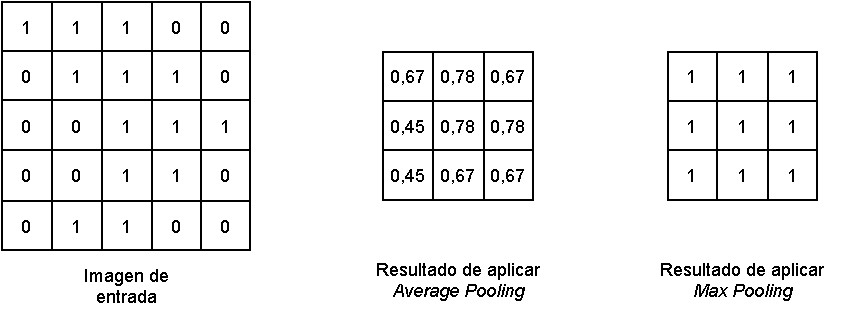
\includegraphics[width=0.95\textwidth]{figuras/desarrollo teorico/Pooling.pdf}
\caption{Aplicación de \textit{Pooling} de tamaño 3x3 a imagen de entrada 5x5 con \textit{stride} de 1}
\label{fig:pooling}
\end{figure}

Por último, para completar el proceso para la clasificación de imágenes, nos encontramos las capas de salida que son \textbf{Capas Totalmente Conectadas} o \textbf{\textit{Fuly Connected Layers}} (FL). Estas se sitúan al final de la arquitectura de la red, para convertir los \textit{feature maps} en vectores unidimensionales. Estas trabajan como una red neuronal tradicional y tienen como fin, acabar la clasificación de las imágenes de entradas en función de los valores de las características extraídas por los \textit{feature maps}.


\subsection{Arquitecturas}

Para conocer el desarrollo de las redes neuronales convolucionales, se va a tomar como referencia el desafío anual \textit{ImageNet Large Scale Visual Recognition} (ILSVRC) \cite{russakovsky2015imagenet}. En este desafío, se muestran desarrollos realizados en todo el mundo, donde diferentes arquitecturas compiten por ser la mejor y más preciso a la hora de clasificar y detectar objetos sobre la base de datos de \textit{ImageNet} \cite{5206848}. Este conjunto de datos, es uno de los más grandes existentes en la actualidad, con más de 14 millones de imágenes etiquetadas manualmente, con más de 20000 categorías diferentes. 

Algunas de las redes más importantes en los últimos años presentadas en este reto son:

\begin{itemize}
    \item \textbf{AlexNet: \cite{NIPS2012_c399862d}} Nacida en el año 2012 fue la primera vez que ganó el reto una arquitectura basad en CNN. Este año la tasa de error cometida bajó de manera considerable en comparación a años anteriores, pasando del 25\% al 17\% de error. 
    
    AlexNet era una red más compleja que las empleadas hasta el momento, y estaba compuesta por 5 capas convolucionales, 3 capas de \textit{pooling}y 3 capas \textit{fully connected} al final. Esta tenía 60 millones de parámetros y en este año se tardó en entrenar 6 días. En la figura \ref{fig:alexnet}, se puede ver una representación de como es la arquitectura de esta red.\\
    
    \begin{figure}[!h]
        \centering
        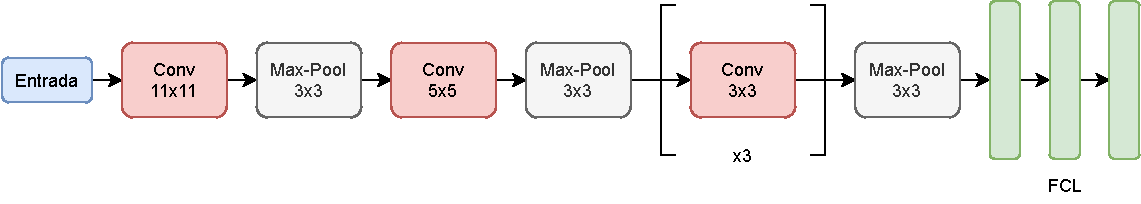
\includegraphics[width=\textwidth]{figuras/desarrollo teorico/desarrollo_teorico-AlexNet.pdf}
        \caption{Arquitectura de la red neuronal convolucional AlexNet}
        \label{fig:alexnet}
    \end{figure}
    
    En esta red, se implementa la función de activación ReLU, que hasta el momento no estaba siendo empleada. Esto aceleró de manera drástica el proceso de entrenamiento hasta en 6 veces en comparación a usar \textit{tanh} o \textit{sigmoid}, sin perder precisión.
    
    Además cabe destacar también la implementación de dos técnicas bastante novedosas para el momento: el \textit{Data Augmentation} (DA) y la técnica del \textit{Dropout} \cite{JMLR:v15:srivastava14a}. Ambas técnicas son empleadas para tratar que la red no sufra de \textit{overfitting}, pero atacando el problema desde diferentes puntos. Con el \textit{Data Augmentation}, se aumenta se añaden perturbaciones en las imágenes originales, consiguiendo una mayor cantidad de imágenes de entrenamiento. Estas perturbaciones son por ejemplo, realizar ampliaciones, rotaciones, modificar la iluminación, etc. Por otro lado, la técnica del \textit{Dropout} consiste en eliminar cierto porcentaje de neuronas de manera aleatoria de la red, haciendo que esta le cueste más aprender, y por tanto, impedir que sobreaprenda los ejemplos de los datos de entrenamiento.
    
    \item \textbf{VGGNet \cite{simonyan2015deep}:} Es el finalista del reto en 2014 y desde entonces ha sido una arquitectura ampliamente influyente. Este demostró de manera bastante intuitiva como debe ser la profundidad de una arquitectura de una red, para que trabaje de manera adecuada, ya que esto es lo que le permite extraer detalles a diferentes niveles de la imagen. Esta consiguió una tasa de error del 7,2 \%.
    
    Además, su arquitectura es bastante simple, formándose por 19 capas convolucionales con tamaños de filtro de 3x3 y \textit{stride} de 1, y capas de \textit{max pooling} con \textit{stride} de 2. En la figura \ref{fig:vggnet}, se puede ver como es la arquitectura de esta red.\\
    
    \begin{figure}[!h]
        \centering
        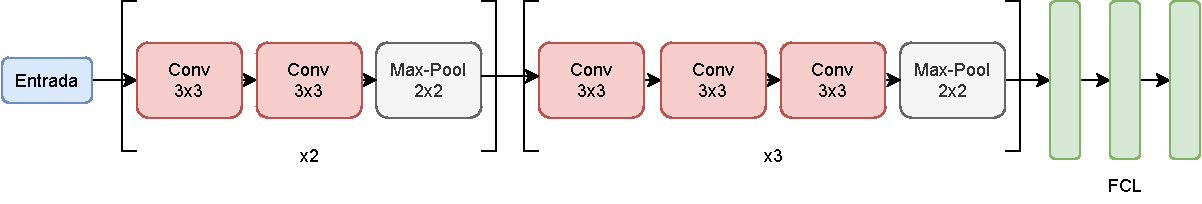
\includegraphics[width=1.05\textwidth]{figuras/desarrollo teorico/desarrollo_teorico-VGG16.pdf}
        \caption{Arquitectura de la red neuronal convolucional VGGNet}
        \label{fig:vggnet}
    \end{figure}
    
    Por otro lado, también se publicó de manera libre la configuración de los pesos que se han utilizado, por lo que sirve como base para el desarrollo de diferentes aplicaciones sin necesidad de grandes entrenamientos.
    
    \item \textbf{GoogLeNet (Inception V1): \cite{szegedy2014going}} Fue la ganadora del reto en el año 2014. Fue desarrollada por Google, pero sus autores hacen tributo a la arquitectura LeNet, en la cual se basaron en gran parte para el desarrollo de esta. Arrojó un error del 6,7 \%. Por debajo de la anteriormente comentada VGGNet.
    
    La arquitectura de esta red es bastante compleja en comparación con las existentes hasta el momento, ya que fue un modelo bastante diferente al general que había sido presentado hasta entonces. En esta se disponen varios bloques, donde se realizan diversas operaciones en paralelo, en vez de en forma secuencial como se había estado haciendo hasta este momento. En la figura \ref{fig:googlenet}, se puede ver como es la arquitectura de esta red.
    
    En esta red, se introduce por primera vez el módulo de \textbf{Inception}, que es sacado de un trabajo anterior \cite{szegedy2014going}. Un módulo Inception tiene la forma presentada en la figura \ref{fig:inception_bloque}.
    
    \begin{figure}[!h]
        \centering
        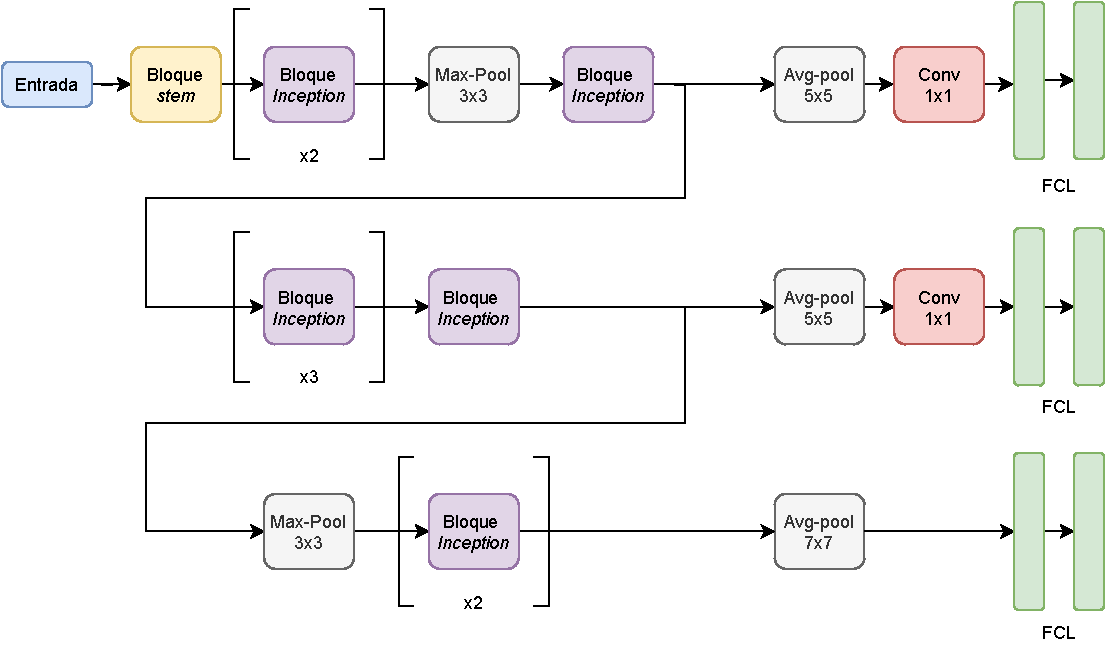
\includegraphics[width=1\textwidth]{figuras/desarrollo teorico/desarrollo_teorico-Inception V1.pdf}
        \caption{Arquitectura de la red neuronal convolucional GoogLeNet (Inception V1)}
        \label{fig:googlenet}
    \end{figure}
    
    \begin{figure}[!h]
    \centering
    \begin{subfigure}{0.45\textwidth}
        \centering
        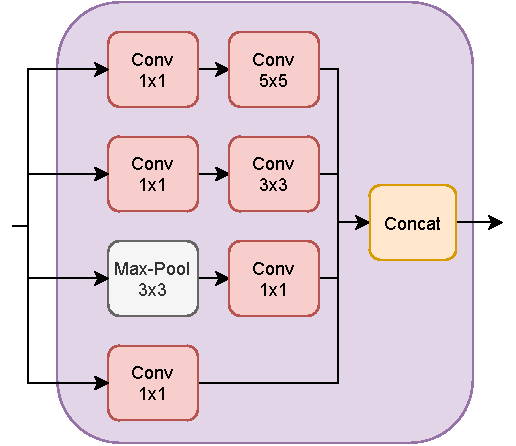
\includegraphics[width=\textwidth]{figuras/desarrollo teorico/desarrollo_teorico-Inception V1-inception.pdf} 
        \caption{Bloque \textit{Inception}}
        \label{fig:inception_bloque}
    \end{subfigure}
    \hfill\\
    \begin{subfigure}{0.65\textwidth}
        \centering
        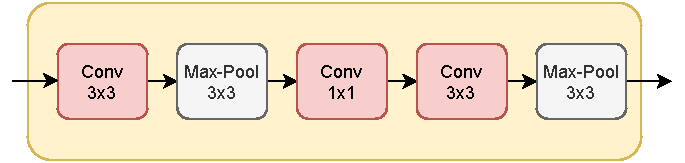
\includegraphics[width=\textwidth]{figuras/desarrollo teorico/desarrollo_teorico-Inception V1-stem.pdf} 
        \caption{Bloque \textit{stem}}
        \label{fig:stem_bloque}
    \end{subfigure}
    \caption{Bloques componentes de la arquitectura GoogleNet (Inception V1)}
    \label{fig:bloques_inceptionv1}
    \end{figure}
    
    Como se puede ver, ya no se aplica de forma secuencial la serie tradicional de capas convolucionales a la que se estaba acostumbrado, sino que el procesamiento se realiza de forma paralela, concatenando definitivamente estos procesos. Además se puede observar como realmente la aplicación de esto, no aumenta en gran medida el número de parámetros de la red y esto es debido a la aplicación de convoluciones de tamaño 1x1 que reducen de manera significativa el tamaño de la imagen de entrada. También introduce la eliminación de la capa \textit{fully connected}, sustituyéndolo por lo que llaman \textit{global average media}, que consiguiendo reducir el error en la precisión hasta en un 0,6\%.
    
    
    \item \textbf{ResNet: \cite{He2016}} Fue la ganadora del reto en el año 2015 y fue desarrollada por Microsoft. Este trabajo fue el primero en presentar redes basados en bloques residuales. Consiguió en este año bajar la tasa de error hasta un 3,57 \%, lo que marcó un gran hito en este ámbito, ya que las personas en tareas similares suelen tener una tasa de error entre el 5\% y el 10\%, dependiendo de las habilidades y experiencias de cada persona. No solo eso sino que con este concepto, se llegó a generar una red con 152 capas que era menos compleja de entrenar que la anteriormente comentada VGGNet que tan solo contaba con 19 capas de profundidad. En la figura \ref{fig:resnet}, se puede ver como es la arquitectura de esta red.
    
    \begin{figure}[!h]
        \centering
        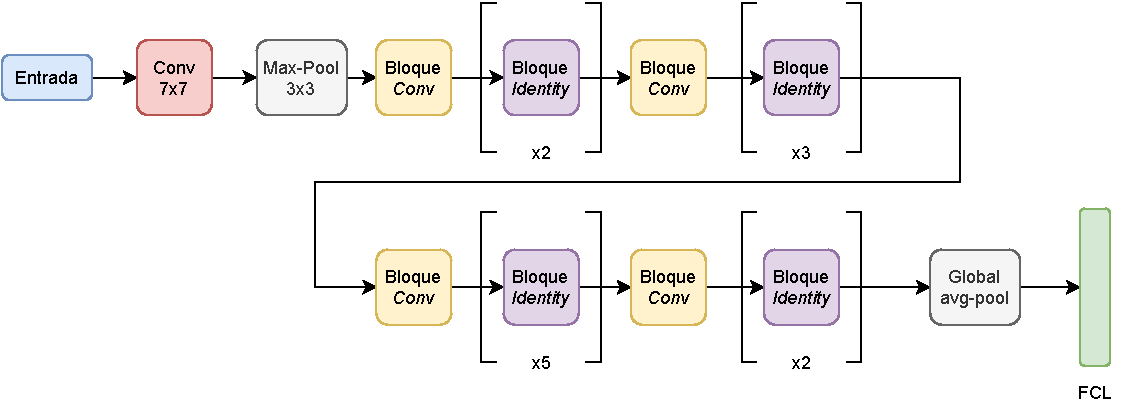
\includegraphics[width=\textwidth]{figuras/desarrollo teorico/desarrollo_teorico-ResNet 50.pdf}
        \caption{Arquitectura de la red neuronal convolucional ResNet-50}
        \label{fig:resnet}
    \end{figure}
    
    \begin{figure}[h]
    \centering
    \begin{subfigure}{0.55\textwidth}
        \centering
        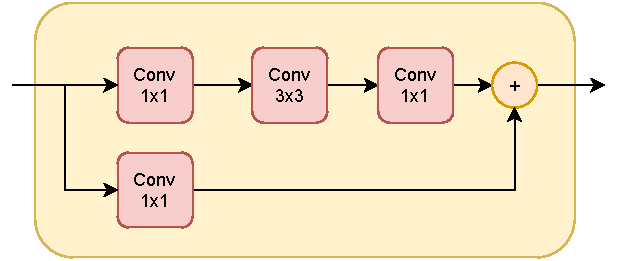
\includegraphics[width=\textwidth]{figuras/desarrollo teorico/desarrollo_teorico-ResNet 50-conv.pdf} 
        \caption{Bloque \textit{conv}}
        \label{fig:conv_bloque}
    \end{subfigure}
    \hfill
    \begin{subfigure}{0.55\textwidth}
        \centering
        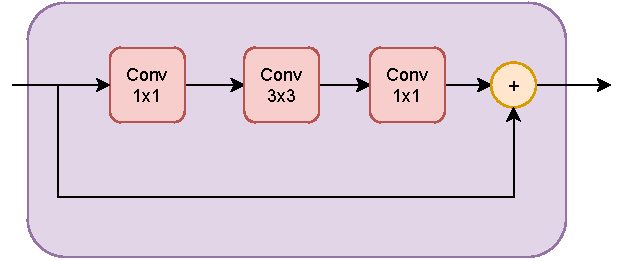
\includegraphics[width=\textwidth]{figuras/desarrollo teorico/desarrollo_teorico-ResNet 50-identity.pdf} 
        \caption{Bloque \textit{identity}}
        \label{fig:identity_bloque}
    \end{subfigure}
    \caption{Bloques componentes de la arquitectura ResNet-50}
    \label{fig:bloques_resnet50}
    \end{figure}

    
    La idea básica en la que se centra ResNet, es el tratar de dejar de apilar capas, si se esta viendo que a partir de cierto puntoesto no hace mejorar la precisión en el entrenamiento. De hecho plantean la aparición de problemas como el \textit{vanishing gradient} o el \textit{curse of dimensionality} donde la red dejaría de aprender por estos motivos.
    
    A partir de este punto nace la idea de los bloques residuales, que básicamente es una conexión que salta un cierto número de capas. En la figura \ref{fig:bloque_residual}, se puede observar como se realiza esta conexión.
    
    \begin{figure}[!h]
        \centering
        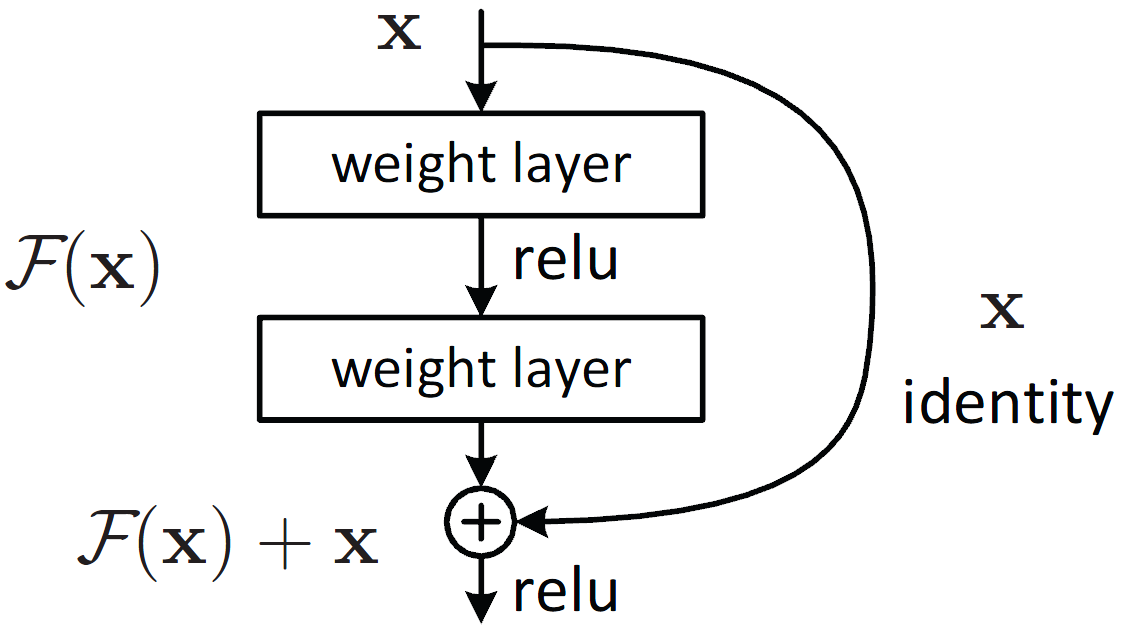
\includegraphics[width=0.5\textwidth]{figuras/desarrollo teorico/bloque_residual.png}
        \caption{Arquitectura del bloque residual \cite{He2016} propuesto para arquitecturas ResNet}
        \label{fig:bloque_residual}
    \end{figure}
    
    La idea tras estos bloques residuales, radica en introducir cierta variación en la imagen de entrada, tratando de conservar el procesado y los detalles de la imagen de entrada, junto a su contexto, que de no tener esta conexión residual, se desvanece con la profundidad de la red.
    
    
\end{itemize}  % INCLUDE: desarrollo teórico
% !TEX root = ../my-thesis.tex
%
\chapter{PROBLEMA A RESOLVER}
\label{sec:problema}

Una vez conocido el estado del arte de la clasificación de malas hierbas y habiendo presentado las bases teóricas del trabajo, se va a pasar a desarrollar en mayor profundidad el problema que motiva este trabajo y la hipótesis de partida para tratar de solucionarlo. Posteriormente, se presentará el conjunto de datos (\textit{datasetç}) seleccionado con el que se comprobará esta hipótesis planteada.

\section{Problema localizado e hipótesis para su resolución}

Como ya se introducía en el estado del arte, en la actualidad, dentro del campo de la agricultura, la agricultura de precisión está tomando bastante protagonismo en los últimos años, debido a las ventajas que supone, económica y medio-ambientalmente. Esto está llevando a crear grandes desarrollos en este área, donde se descubren nuevas barreras tecnológicas que deben ser superadas para la implantación de ciertos sistemas automatizados en el campo.

Uno de estos campos, es la detección y eliminación de malas hierbas, ya ya que estas compiten con la cosecha por los recursos que aportar el campo, lo que limita de gran manera la producción total, por lo que en la actualidad, se trata de realizar trabajos de eliminación de estas plagas de forma extensiva. Esto no es una forma adecuada de aplicarse, debido a que podría afectar al desarrollo del cultivo, además de que se emplean grandes cantidades de correctivos que no son realmente necesarios.

La solución que se propone por tanto, es la localización y clasificación de forma precisa de estas malas hierbas en los cultivos de forma automatizada, aplicando correctivos de forma puntual a estas de forma selectiva y eficaz a cada una de ellas. Para esto, se ha trabajado en los últimos años en desarrollos donde se trata de emplear las últimas técnicas de clasificación de imágenes para abordar las dificultades y problemáticas de la clasificación de diferentes tipos de plantas.

Una de estas técnicas, cada vez está más estandarizada, es el uso de redes neuronales convolucionales, las cuales son entrenadas con un conjunto de datos de muestra etiquetadas, siendo capaces de extraer propiedades visuales de cada uno de los tipos de plantas para posteriormente clasificarlas de forma correcta. Para esto, se emplean redes como las presentadas en el capítulo anterior, las cuáles son arquitecturas genéricas capaces de clasificar de forma eficiente gran número de tipos de imágenes, empleando grandes conjuntos de datos con los que son entrenadas,  que conlleva grandes tiempos de entrenamiento asociados y amplia capacidad computacional de lo cual, no siempre se dispone. Para ello, se propone la solución de usar estas redes pre-entrenadas, de manera que inicialmente ya son capaces de clasificar una elevada cantidad de tipos de imágenes, por lo que luego solo es necesario re-entrenarlas con el \textit{dataset} objetivo, con menores tiempos de entrenamiento \cite{Olsen2019}.

Esta técnica trae varias problemáticas consigo. Una de ellas es que estas redes, para poder tener la capacidad de clasificar numerosos tipos de imágenes, tienen que tener tamaños excesivamente grandes, tanto en número de capas como de parámetros, y la tendencia en los últimos años es que sigan creciendo. En la Tabla \ref{tab:tamaño_cnn}, se pueden ver algunos ejemplos de los tamaños de estas redes.

\begin{table}[h]
\caption{Tamaño de algunas de las CNNs más empleadas en los últimos años}
\label{tab:tamaño_cnn}
\centering
\begin{tabular}{l|r|r}
\toprule
\multicolumn{1}{c|}{\textbf{Red Neuronal Convolucional}} & \multicolumn{1}{c|}{\textbf{Número de capas}} & \multicolumn{1}{c}{\textbf{Parámetros}} \\ \hline
LeNet \cite{lesnet}                                                    & 5                                             & $60 \cdot 10^3$                                   \\
AlexNet \cite{NIPS2012_c399862d}                                                 & 8                                             & $62 \cdot 10^6$                                \\
VGG-16 \cite{simonyan2015deep}                                                   & 16                                            & $138 \cdot 10^6$                               \\
Inception V1 \cite{szegedy2014going}                                            & 22                                            &  $7 \cdot 10^6$                                 \\
Inception V3 \cite{szegedy2015rethinking}                                             & 159                                           & $23 \cdot 10^6$                                \\
Resnet-50 \cite{He2016}                                               & 50                                            & $25 \cdot 10^6$         \\
\bottomrule
\end{tabular}
\end{table}

Lo anterior puede ser válido si estas redes van a ser ejecutadas en equipos con gran potencia computacional, pero es una gran limitación si se quieren emplear en \textit{edge devices}, los cuáles no cuentan con una amplia potencia computacional capaz de mover grandes redes en tiempo adecuados. Además cuenta con otra desventaja, que es el gran número de datos que son necesarios para entrenar estas redes tan ``genéricas''. Además, al tener tamaños más grandes, estas redes son más complicadas de analizar y conocer su comportamiento real, debido al gran número de parámetros que entran en el juego de estas.

Para esto, se pretende buscar una manera de obtener CNNs de menor tamaño, más especializadas, más rápidas e igual de eficientes a la hora de clasificar un \textit{dataset} dado. Para ello, se cree que una opción adecuada de optimizar la arquitectura de estas redes es empleando algoritmos de optimización como son los Algoritmos Evolutivos, más específicamente, los Algoritmos Genéticos. Estos tienen gran un rendimiento a la hora de optimizar grandes problemas que con otros algoritmos ha sido complicado llegar a una solución válida, por lo que se intuye que pueden ser de gran ayuda para la resolución del problema anteriormente comentado.

Como se puede observar, este es un trabajo que puede servir en numerosos campos donde la clasificación de imágenes es un punto crítico y que debe ser optimizado. Aún así, este trabajo en particular se centrará específicamente en el la clasificación de diferentes tipos de malas hierbas.

Por tanto, en este trabajo se tratará de verificar si la hipótesis realizada es cierta y si empleando Algoritmos Genéticos para el diseño de nuevas arquitecturas de CNNs, las realizan de manera que sean más pequeñas, más especializadas y más rápidas manteniendo un desempeño similar al que se obtiene con las soluciones actuales.

\section{Datos a clasificar}

Para alcanzar el objetivo de este trabajo, se debe tener una base de datos suficientemente grande y con cierta calidad, para poder comprobar el desempeño de las arquitecturas extraídas. Es por ello que se seleccionó el \textit{dataset} publicado para el desarrollo de aplicaciones de clasificación de diferentes clases de malas hierbas nativas en Australia \cite{Olsen2019}.

Este \textit{dataset}, cuenta con un total de 17509 imágenes clasificadas, donde se recogen un total de 8 especies diferentes de malas hierbas y un conjunto separado de plantas que no son malas hierbas, denominados negativos. Estas han sido recopiladas de diferentes lugares de Australia como se puede observar en la Figura \ref{fig:loc_malas_hierbas}. Estas especies seleccionadas están localizadas más específicamente en las siguientes zonas de pastoreo a lo largo del estado de Queesland: ``Black River'', ``Charters Towers'', ``Cluden'', ``Douglas'', ``Hervey Range'', ``Kelso'', ``McKinlay'' y ``Paluma''.

Este \textit{datset} incluye imágenes etiquetadas de las siguientes especies: ``Chinee apple'', ``Snake weed'', ``Lantana'', ``Prickly acacia'', `` Siam weed'', ``Parthenium'', ``Rubber vine'' y ``Parkinsonia''. Una recopilación de algunas de las imágenes de cada especie puede verse en la figura \ref{fig:dataset_ejemplo_grande}.

Esta amplia recopilación de imágenes permitirá distinguir entre diferentes tipos de malas hierbas, además de diferenciarlas de aquellas que no lo son, de manera que se podrá comprobar el rendimiento de las arquitecturas obtenidas con el desarrollo del algoritmo planteado durante este trabajo.

\begin{figure}[h]
    \centering
    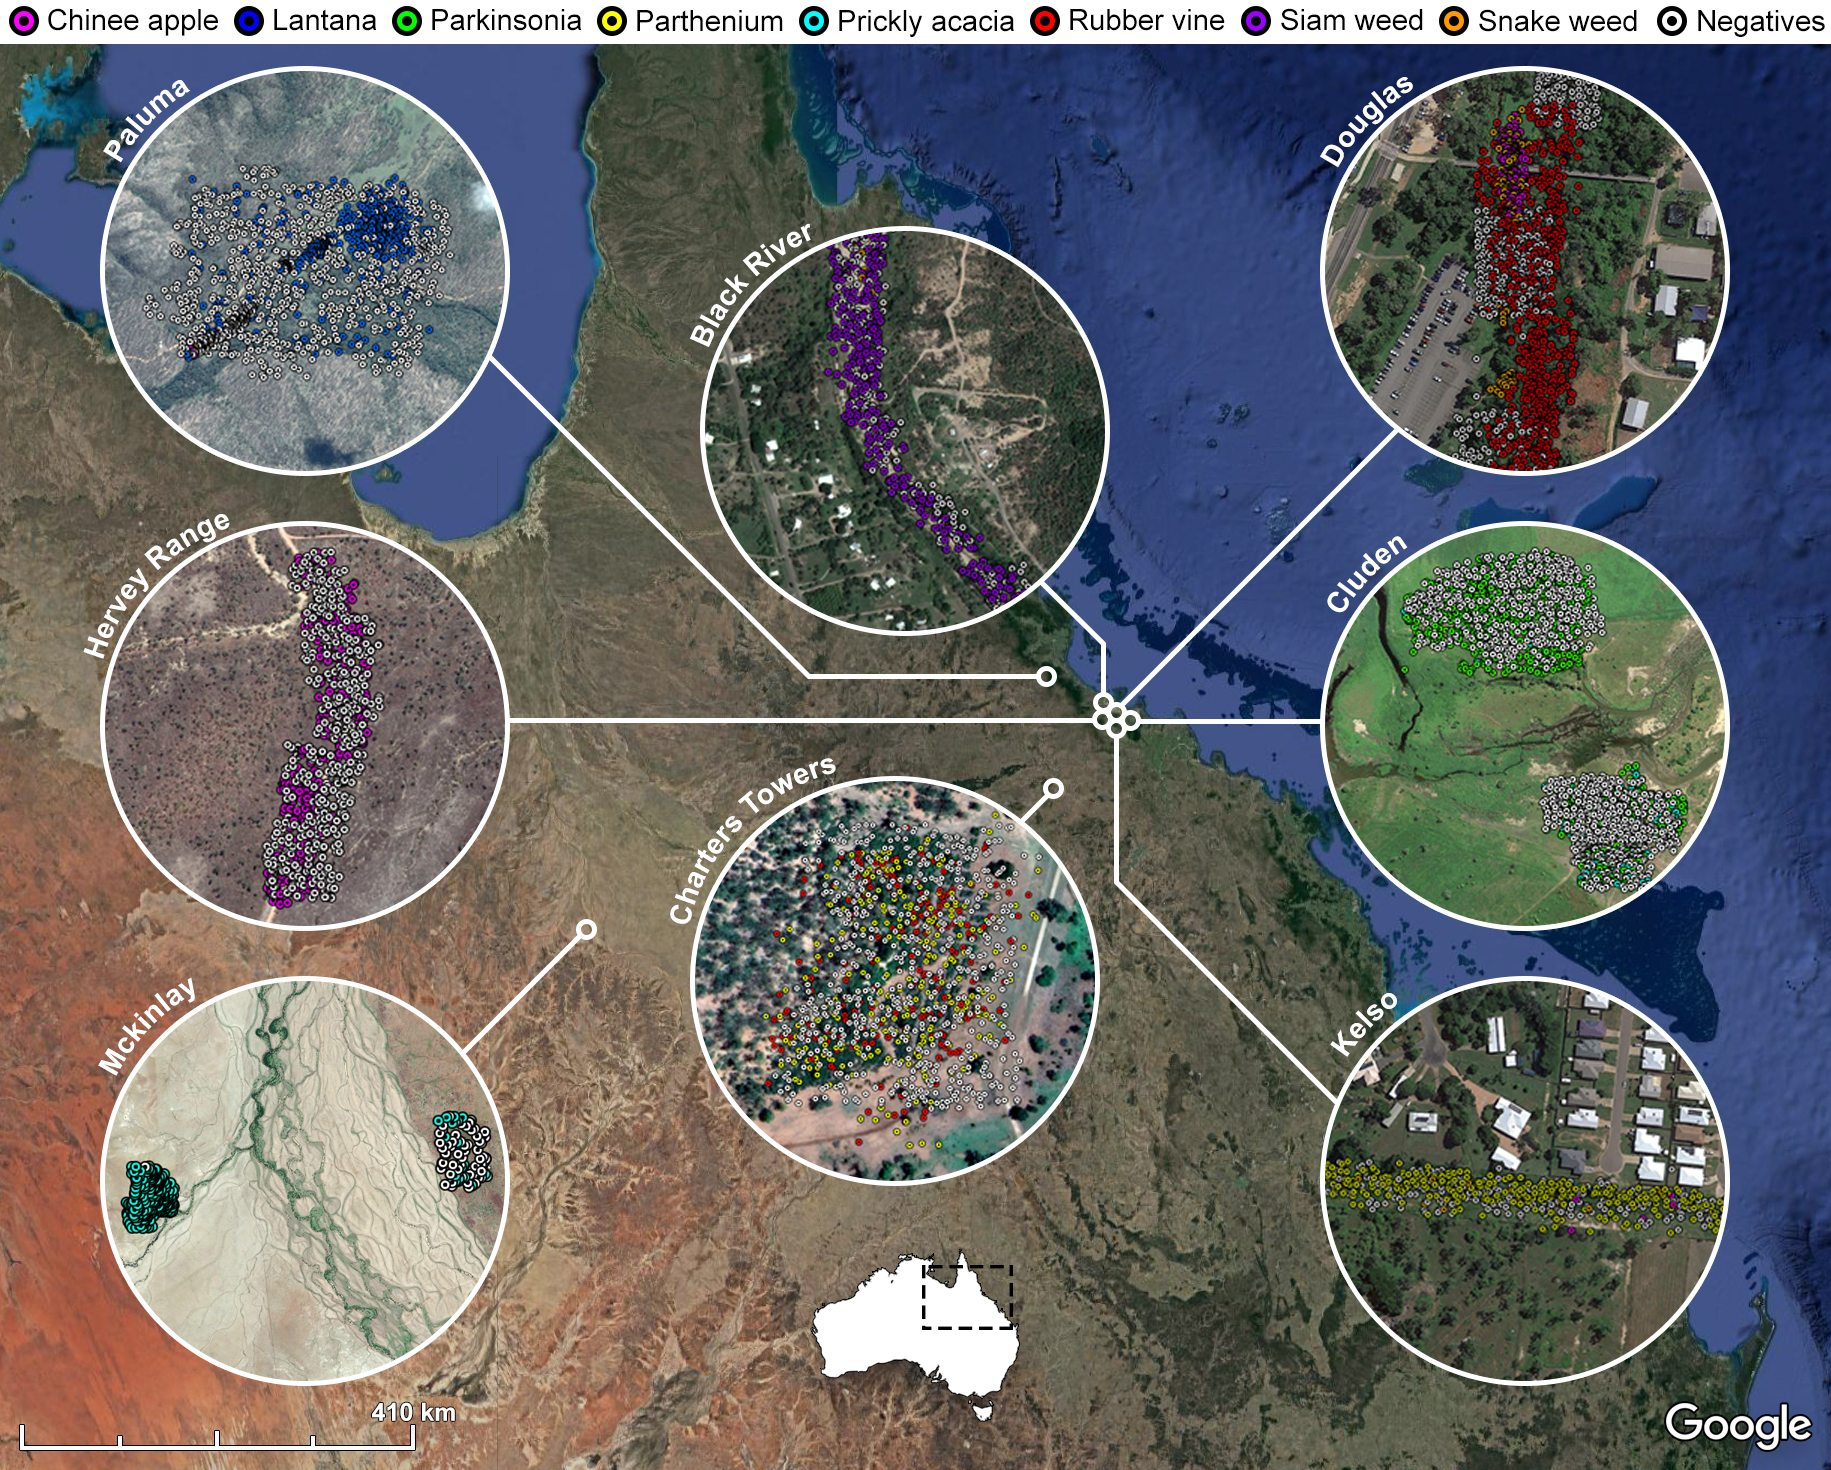
\includegraphics[width=0.95\textwidth]{figuras/problema/localizacion_malas_hierbas.jpg}
    \caption{Localización de las imágenes etiquetadas de malas hierbas del \textit{dataset} seleccionado \cite{Olsen2019}}
    \label{fig:loc_malas_hierbas}
\end{figure}

\begin{figure}[!h]
\centering
    \begin{subfigure}{0.24\textwidth}
        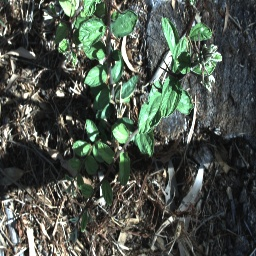
\includegraphics[width=\textwidth]{figuras/problema/chinee_apple.jpg}
        \caption{Chinee Apple}
    \end{subfigure}
    \hfill
    \begin{subfigure}{0.24\textwidth}
        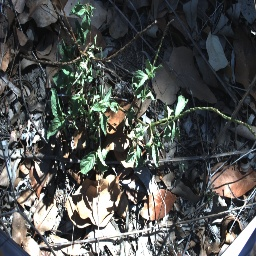
\includegraphics[width=\textwidth]{figuras/problema/snake_weed.jpg}
        \caption{Snake Weed}
    \end{subfigure}
    \hfill
    \begin{subfigure}{0.24\textwidth}
        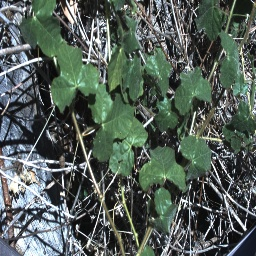
\includegraphics[width=\textwidth]{figuras/problema/lantana.jpg}
        \caption{Lantana}
    \end{subfigure}
    \hfill
    \begin{subfigure}{0.24\textwidth}
        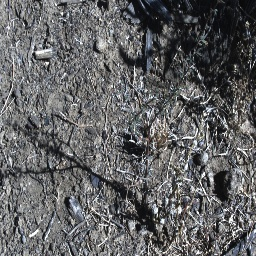
\includegraphics[width=\textwidth]{figuras/problema/prickly_acacia.jpg}
        \caption{Prickly Acacia}
    \end{subfigure}
    \hfill
    \begin{subfigure}{0.24\textwidth}
        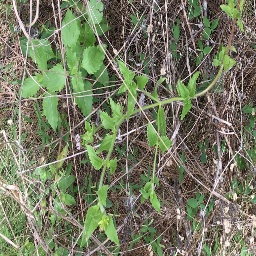
\includegraphics[width=\textwidth]{figuras/problema/siam_weed.jpg}
        \caption{Siam Weed}
    \end{subfigure}
    \hfill
    \begin{subfigure}{0.24\textwidth}
        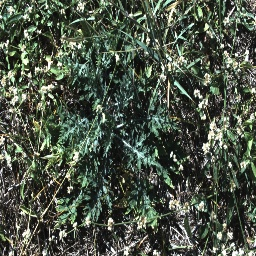
\includegraphics[width=\textwidth]{figuras/problema/parthenium.jpg}
        \caption{Parthenium}
    \end{subfigure}
    \hfill
    \begin{subfigure}{0.24\textwidth}
        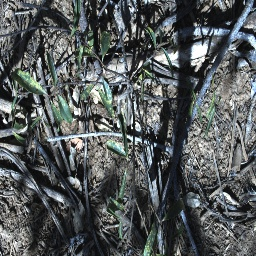
\includegraphics[width=\textwidth]{figuras/problema/rubber_vine.jpg}
        \caption{Rubber Vine}
    \end{subfigure}
    \hfill
    \begin{subfigure}{0.24\textwidth}
        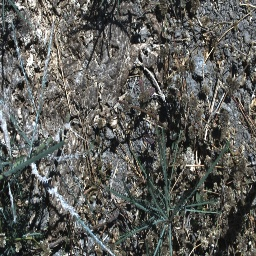
\includegraphics[width=\textwidth]{figuras/problema/parkinsonia.jpg}
        \caption{Parkinsonia}
    \end{subfigure}
    \caption{Imágenes de las diferentes especies recogidas en el \textit{dataset}}
    \label{fig:dataset_ejemplo_grande}
\end{figure}

  % INCLUDE: problema
% !TEX root = ../my-thesis.tex
%
\chapter{IMPLEMENTACIÓN DESARROLLADA}
\label{sec:implementación}

A lo largo de este capítulo, se desarrollará y explicará como se ha realizado la implementación de los diferentes algoritmos, que harán posible desarrollar posteriormente las pruebas y experimentos pertinentes para la verificación de la hipótesis y solución del problema que se desarrolla en este trabajo.

\section{Algoritmo Genético}

En primer lugar, se va a pasar a desarrollar como se ha realizado la elaboración del algoritmo genético, el cual tiene como fin optimizar la arquitectura de las redes de neuronales convolucionales.

Esto se realizará por medio de la librería elaborada en Python, \textbf{DEAP} (\textit{Distributed Evolutionary Algorithms in Python}) \footnote{\url{https://deap.readthedocs.io/en/master/}}. Esta es una librería ampliamente utilizada para el desarrollo de algoritmos evolutivos, como se puede ver en su página web. Esto es debido a su gran personalización y a la gran cantidad de representaciones aceptadas y algoritmos implementados dentro de la librería.

Se ha seleccionado esta librería mayoritariamente por su filosofía, ya que en vez de emplear inicializadores cerrados como en otras librerías disponibles, se nos solicita explícitamente cada uno de los parámetros del algoritmos, que son además, fácilmente modificables e integrables con el resto del software, adaptándose adecuadamente al problema que se trata de resolver. Además, el algoritmo esta totalmente disponible para su modificación, en caso de querer o requerir establecer una dinámica única del algoritmo evolutivo.

En este caso se va a partir de la implementación realizada en esta librería para un algoritmo genético de objetivo único, el cual, como se verá a lo largo de este capítulo, sufrirá de algunos cambios para realizar la ejecución de manera adecuada para resolver el problema dado.

Este va a seguir la estructura mostrada en la figura \ref{fig:esquema_funcional_GA}, y se desarrollarán cada uno de sus puntos a lo largo de este capítulo.\\

\begin{figure} [h]
    \centering
    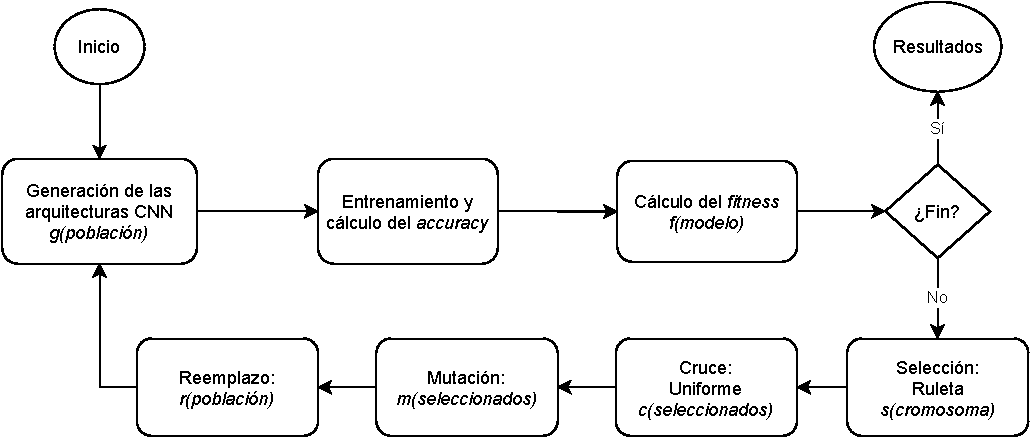
\includegraphics[width=\textwidth]{figuras/implementacion/esquema_funcionamiento.pdf}
    \caption{Esquema de funcionamiento de la implementación desarrollada del Algoritmo Genético}
    \label{fig:esquema_funcional_GA}
\end{figure}

\subsection{Codificación del problema}

La codificación del problema es uno de los puntos más delicados a la hora de desarrollar el algoritmo genético en cuestión como ya se ha visto en el desarrollo teórico.

En este caso, se ha planteado una codificación binaria basada en la selección de diferentes parámetros y configuraciones para cada una de las capas que conforman la arquitectura de la red neuronal convolucional.

Para ello, se ha seleccionado una codificación de \textbf{10 bits} para cada una de las capas de la red, donde se configurarán cada una de las propiedades que tiene esta. Posteriormente, cada una de estas capas de concatenarán formando finalmente la arquitectura de la red completa, donde como parámetro del algoritmo se deberá especificar el número de capas que formarán la arquitectura de la red definitiva.\\

\begin{table}[h]
\caption{Codificación de una capa de la CNN para el Algoritmo Genético}
\label{tab:codificacion}
\centering
\begin{tabular}{l|llllllllll}
\toprule
\textbf{Tipo}               & \multicolumn{10}{c}{\textbf{Posición de los genes}}                         \\
\textbf{de capa}            & \textbf{0} & \textbf{1} & \textbf{2}     & \textbf{3}     & \textbf{4}     & \textbf{5}     & \textbf{6}      & \textbf{7}      & \textbf{8}    & \textbf{9} \\ \hline
\textit{Vacía}              & 0 & 0 & x     & x     & x     & x     & x      & x      & x    & x \\
\textit{Pooling}            & 0 & 1 & $T$     & $K$     & x     & x     & x      & x      & x    & $S$ \\
\textit{Convolucional}        & 1 & 0 & $K_{x1}$ & $K_{x2}$ & $K_{y1}$ & $K_{y2}$ & $FMS_1$ & $FMS_2$ & $A_T$ & $S$ \\
\textit{Convolucional Residual} & 1 & 1 & $K_{x1}$ & $K_{x2}$ & $K_{y1}$ & $K_{y2}$ & $FMS_1$ & $FMS_2$ & $A_T$ & $S$ \\
\bottomrule
\end{tabular}
\end{table}

En la Tabla \ref{tab:codificacion}, se puede observar como es el esquema de codificación de cada una de las capas de la red neuronal. En ella se puede observar como se componen cada una de estas capas, donde se distinguen cuatro tipos de capas: \textit{Vacía}, \textit{Pooling}, \textit{Convolucional} y \textit{Convolucional Residual}. Estas vienen codificadas por dos genes que marcan el tipo de capa, que son las dos primeras que se encuentras en la codificación del problema.

Esta codificación además cuenta con numerosas ventajas, como el poder implementar redes anteriormente presentadas tales como VGG-16 y ResNet-50 como posibles individuos en la población, o de otra forma, de ser las mejores arquitecturas en el espacio de búsqueda, aparecer como solución.

A continuación, se va a pasar a desarrollar cuál es el significado de cada uno de los parámetros de cada tipo de capa que forman el genotipo del Algoritmo Genético propuesto.

\begin{itemize}
    \item \textbf{Capa vacía:} Esta tipo de capa es la más simple, y se implementa para poder codificar arquitecturas de diferente profundidad de capas. Es por ello que en la concatenación de capas puede aparecer una capa vacía la cuál no realizará ningún proceso, por lo que se podrán generar arquitecturas con menor número de capas que las seleccionadas.
    
    \item \textbf{\textit{Capa de Pooling}:} Esta se trata de una capa de tipo \textit{Pooling} como las que se presentaron en las bases teóricas del trabajo. Esta consta de tres parámetros principales para su configuración, que son: $T$, $K$ y $S$, que a continuación se pasará a su explicación.
    
    \begin{itemize}
        \item \textit{Tipo de Pooling} ($T$) :  Este parámetro hace referencia al tipo de operación de \textit{Pooling} que se va a realizar en esta capa. Se han seleccionado dos operaciones posibles para esta capa que son: \textbf{\textit{Average Pooling}} y \textbf{\textit{Max Pooling}}.
        
        \item \textit{Tamaño del filtro (kernel)} ($K$) : Este parámetro hace referencia al tamaño del filtro que se introducirá en esta operación. Este tendrá un tamaño cuadrado y un tamaño de \textbf{2 o 3 píxeles}.
        
        \item \textit{Stride} ($S$) : Este hace referencia al paso con el que se va recorriendo el filtro o \textit{kernel} a lo largo de la imagen de entrada. Se pueden dar dos casos, que se realice son \textit{stride} de \textbf{2 o de 3 píxeles}.
        
    \end{itemize}
    
    Como se puede observar, empleando este tipo de codificación, es posible que en algunos casos se de la problemática de situarse varias capas de \textit{Pooling} de forma consecutiva, cosa que no tiene sentido a la hora de generar la estructura de la red. Es por ello que, de producirse numerosas capas de este tipo de forma seguida, solo se tendrá en cuenta la primera, ignorándose las siguientes capas de \textit{Pooling} que vayan apareciendo posteriormente.
    
    \item \textbf{Capa Convolucional:} Esta se trata de una capa convolucional. Esta es algo más compleja que lo que se veía para las capas de tipo \textit{Pooling} ya que existen muchos más parámetros ajustables dentro de ellas, y muchas más combinaciones como se pueden ver por ejemplo en las redes VGG-16 o ResNet-50. 
    
    Otra puntualización, es que en este tipo de capas, el tamaño del filtro puede ser asimétrico como sucede por ejemplo en las redes con bloques de tipo Inception. Para dar mayores posibilidades a las arquitecturas que se pueden generar, se introducirá de la misma manera la posibilidad de codificar este tipo de filtros asimétricos.
    
    Esta capa convolucional se puede configurar por un mayor número de parámetros que otras redes y estas vienen codificadas por los parámetros: $K_{x}$, $K_{y}$, $FMS$, $A_T$ y $S$, que a continuación van a ser explicados.
    
    \begin{itemize}
        \item \textit{Tamaño del filtro en dirección horizontal} ($K_{x}$) : Hace referencia dentro de la capa convolucional seleccionada, al tamaño en dirección horizontal que puede tomar el filtro. Este consta de 2 bits para su codificación, por lo que se pueden generar hasta cuatro combinaciones de tamaños. El tamaño final, por tanto viene dado por la siguiente expresión:
        
        \begin{equation}
            \textit{Kernel Size} = \text{dec}(K_x) \cdot 2 + 1
        \end{equation}
        
        dando como resultado, la posibilidad codificar tamaños filtros de \textbf{1, 3, 5 y 7}.
        
        \item \textit{Tamaño del filtro en dirección vertical} ($K_{y}$) : Este funciona de manera análoga a como lo hace $K_x$ sin diferencia ninguna a la hora de codificar los tamaños de los filtros. La única diferencia radica a que se hace referencia al tamaño del filtro en dirección vertical, consiguiendo de esta manera poder codificar tamaños de filtros no cuadrados.
        
        \item \textit{Número de filtros (Feature Map Size)} ($FMS$) : Este parámetro hace referencia al número de filtros que existirán en cada una de las capas de convolución. Un mayor número de estos, obtendrán mayor cantidad de detalles de la imagen, a cambio de hacer mucho más lenta y pesada esta red, si esta es demasiado voluminosa en las capas iniciales de la red, donde el tamaño de entrada de la imagen aún es demasiado grande. Es por ello que se da la selección entre diferentes posibilidades de números de filtros en esta capa.
        
        Para determinar el número de filtros que tendrá una capa es necesario a partir de la codificación de 2 bits, aplicar las siguientes expresiones:
        
        \begin{equation}
            \textit{Feature Map Size} = 2^P
        \end{equation}
        
        \begin{equation}
            P = \text{dec}(FMS) + 6
        \end{equation}
        
        dando como resultado número de filtros posibles de \textbf{64, 128, 256 y 512}.
        
        \item \textit{Tipo de Función Activación} ($A_T$) : Este parámetro hace referencia al tipo de activación que usará posteriormente de haber realizado el proceso de convolución. Para ello existen dos opciones de función de activación: \textbf{\textit{ReLU}} y \textbf{\textit{tanh}}.
        
        \item \textit{Stride} ($S$) : Este es análogo al \textit{stride} que se encontraba en la capa de \textit{Pooling}. Aún así, para este caso cada uno de los bits hacen referencia a pasos diferentes, siendo en una capa de convolución de \textbf{1 o 2 píxeles}. Se ha seleccionado de esta manera para poder imitar el comportamiento de ResNet que huye del uso de capas de \textit{Pooling} y realiza la compresión de la imagen mediante capas de convolución con tamaños de \textit{stride} de 2.
        
    \end{itemize}
    
    Finalmente, tras la generación de cada capa de convolución, se añadirá una capa adicional de \textit{Batch Normalization} \cite{ioffe2015batch} que reduce de forma significativa el tiempo necesario de entrenamiento de la red. De igual manera, para mantener el tamaño de la imagen de entrada al realizar la convolución, es necesario introducir una capa de \textit{Padding} que seguirá la expresión:
    
    \begin{equation}
        P = \frac{K - 1}{2}
    \end{equation}
    
    \item \textbf{Capa Convolucional Residual:} Por último presentar las capas de tipo convolucional residual \cite{He2016}, que vienen introducidas para ayudar al aumento de la profundidad del modelo sin perder el contexto inicial de la imagen y por tanto, la facilidad de entrenamiento de la red.
    
    Los parámetros de configuración de este tipo de capas es exactamente igual especificado para capas convolucionales clásicas. Sin embargo, se deja un lazo abierto justo al crear esta capa que posteriormente será cerrada. Esto sucederá cuando se añada una capa que cumpla los siguientes casos: se añada una nueva capa de \textit{Pooling}, se añada otra capa convolucional residual o se haya llegado al final de codificación.\\
    
    \begin{figure}[h]
    \centering
    \begin{subfigure}{0.8\textwidth}
        \centering
        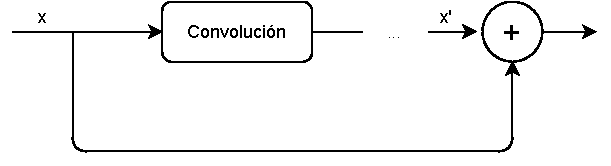
\includegraphics[width=\textwidth]{figuras/implementacion/Skip_convolucion_Implementacion_1.pdf}
        \caption{Capa Residual Identidad}
        \label{fig:residual_identidad}
    \end{subfigure}
    \hfill
    \begin{subfigure}{0.8\textwidth}
        \centering
        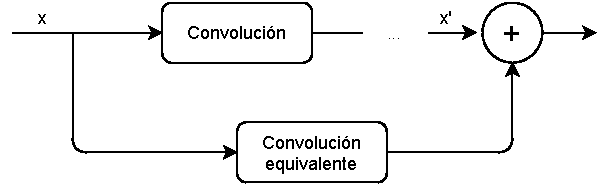
\includegraphics[width=\textwidth]{figuras/implementacion/Skip_convolucion_Implementacion_2.pdf}
        \caption{Capa Residual con capa extra de convolución para satisfacer tamaño de salida}
        \label{fig:residual_conv_eq}
    \end{subfigure}
    \caption{Representación de las posibles configuraciones de capas residuales}
    \label{fig:residual}
    \end{figure}
    
    Debido a la aleatoriedad de generación de este tipo de capas y sobretodo, cuando van a ser cerradas, es posible que se generen tamaños a la hora de realizar la operación de suma o \textit{addition}, que no pueden ser realizados. Para ello se propone la solución que se muestra en la Figura \ref{fig:residual}, donde como se puede observar, en caso de que el tamaño de la imagen \textit{x} sea diferente al tamaño de la imagen \textit{x'}, se genera una convolución equivalente para adaptar este tamaño en la rama residual.
    

\end{itemize}

\subsection{Función \textit{Fitness}}

Tras la generación de la arquitectura de la Red Neuronal Convolucional completa, es necesario realizar una evaluación del desempeño de esta con respecto a los otros individuos de la población, de tal manera que sea posible comparar que tan buena capacidad de clasificación tiene esta. A este valor o número se le denomina \textit{fitness}, como ya se veía en el apartado de las bases teóricas.

Existen diferentes parámetros que consiguen evaluar que tal es rendimiento de la red para la tarea de clasificación de cierto conjunto de datos de prueba etiquetados tras su entrenamiento. Entre ellos, se ha de seleccionar uno o la combinación entre varios, a través de la definición de una expresión entre ellos, que generarán el valor final de \textit{fitness}.

Se ha optado por seleccionar el parámetro \textit{accuracy} del \textit{top 1} como valor de \textit{fitness}, ya que es de los parámetros más extendidos para la comparación y evaluación del desempeño de la redes. Este también es denominado \textit{categorical accuracy} y es el empleado para problemas de clasificación de tipo multi-clase, como el problema que se está resolviendo. Esta se define como:

\begin{equation}
    \text{Accuracy} = \frac{\text{Número de predicciones correctas}}{\text{Número total de predicciones}}
\end{equation}

Además, durante el entrenamiento de las redes, se persigue en obtener el mayor valor de \textit{accuracy} posible, por lo que es adecuado clasificar nuestras redes por este indicador y no por otros como pudieran ser \textit{Precision}, \textit{F1-score} o \textit{Recall}.

\subsection{Selección}

Una vez establecidas las bases del problema en el Algoritmo Genético, se establecerán los diferentes operadores que modificarán a la población a lo largo de numerosas generaciones para conseguir a los mejores individuos.

En primer lugar se va a establecer la operación de selección de los padres que generará a la nueva población. Para ello se ha implementado una operación que se basa en el valor de \textit{fitness} obtenido durante su entrenamiento, dando mayor prioridad a reproducirse a los mejores individuos de la población, pero siempre tratando de conservar a los que podrían llevar algo de carga genética valiosa a pesar de obtener valores de \textit{fitness} menores. Esto asegura que se puedan obtener individuos mejores y además siempre haya oportunidad de explorar de forma uniforme el espacio de búsqueda de las soluciones.

La operación que se ha introducido en particular para esta implementación y que tiene el funcionamiento buscado, es el ya explicado \textbf{Selección por Ruleta} (\textit{Roulette Selection}). Por otro lado, se ha seleccionado una probabilidad de cruce del 90\% tratando de que exista gran cantidad de transpaso de información genética a lo largo de las diferentes generaciones.

\subsection{Cruce}

Una vez seleccionado los pares de individuos, se debe buscar realizar una combinación entre estos que transfiera información valiosa generando nuevos individuos con las propiedades de sus antecesores. Esto se hace mediante la aplicación del cruce como ya se explicó.

En este punto, es necesario ir con cautela a la hora de seleccionar el operador de cruce adecuado, ya que la selección de un mal operador, podría llevar a no generar una alta diversidad de población o que su evolución sea demasiado lenta. Es por ello que se descarta el uso de operadores de cruce tales como el \textit{Single-Point Crossover} o el \textit{Double-Point Crossover}, debido a que no generan gran diversidad en la población resultante.

Por tanto, para el operador cruce se propone el uso del operador de cruce, \textbf{\textit{Uniform Crossover}} que ya se explicó en anteriores capítulos. Este va a transferir información valiosa entre los individuos de forma uniforme a lo largo del genotipo, lo cual lo hace ideal. Se ha seleccionado a su vez una probabilidad de intercambio genético del 20\%, debido a que se debe asegurar que se transfieren parámetros realmente importantes a lo largo de la codificación, y estos resultan ser los dos primeros que seleccionan el tipo de cada capa. Estas resultan ser el 20\% de la codificación total del genotipo.

\subsection{Mutación}

En la operación de mutación, como se ha visto en la teoría, trata de realizar búsquedas de forma aleatoria dentro del espacio de búsqueda, de manera se evite localizarse en óptimos locales a lo largo de esta. Para esta se ha de seleccionar una probabilidad de mutación para cada individuo en cada generación, que decidirá si se le aplica este operador o no. Este ha de ser lo suficientemente bajo para no convertir esta búsqueda, en una búsqueda meramente aleatoria. Es por ello que se ha seleccionado una probabilidad de mutación del 5\%.

Para la selección del operador, al igual que sucedía con la operación de cruce, la mutación se va a realizar de forma uniforme a lo largo de todo el genotipo con una probabilidad de mutación dada. Esta se ha seleccionado de un valor del 20\%, ya que de manera análoga a lo que sucedía en el cruce, este debe ser un valor que asegure que en las pocas veces que se va a producir una mutación, se haga de manera adecuada, y permita un búsqueda en nuevas zonas del espacio de búsqueda de soluciones.

\subsection{Reemplazo}

Finalmente, se da la operación de reemplazo, la cuál se ha implementado una solución bastante sencilla, de manera que se combinan el total de nuevos individuos generados en la nueva generación junto a los individuos de la anterior población ordenados por valor de su \textit{fitness}. De esta lista ordenada, se toman los N valores fijos de población establecidos, que pasarán a ser los nuevos individuos de la nueva población para la siguiente generación.

\subsection{Elitismo}

Debido a la naturaleza del problema y como se ve alterada el \textit{fitness} en función de su correcta evaluación, es necesario asegurar una estrategia de Algoritmo Genético con elitismo. Esto es debido a que el \textit{fitness} se evalúa mediante un proceso de optimización, es posible que no se vea el verdadero potencial de los genes que contiene la arquitectura generada, por lo que se deberá tratar de conservar en su gran medida para asegurar que una vez encontrados un buen genotipo, este no se pierda a lo largo de las generaciones.

Esto se realiza, como ya se explicaba en las bases teóricas, para asegurar que no se pierde al mejor individuo y a su material genético a lo largo de las diferentes poblaciones. Esto unido a los elevados tiempos de ejecución de este tipo de algoritmo, ayuda a una convergencia, aunque sea local, mucho más rápida que si no se tuviera implementado este.

Debido a que la librería DEAP que ha sido la seleccionada para el desarrollo de los Algoritmos Genéticos, no implementa el mecanismo de elitismo de forma nativa, por lo que se ha realizado una modificación en la implementación para añadir este. Para ello, en el proceso de selección, se genera un individuo menos de los que se deberían seleccionar, y finalmente en el proceso de reemplazo, se añade a este individuo dentro de la población nuevamente de forma inalterada.


\section{Redes Neuronales Convolucionales}

Puesto que para analizar la capacidad de clasificación que tiene cada uno de las Redes Neuronales Convolucionales como individuo de la población es necesario realizar un proceso de entrenamiento y de prueba, en esta sección, se desarrollarán las configuraciones que se han realizado para el desempeño de estas redes.

Para realizar la implementación de esta parte, se ha hecho uso de las famosas librerías \textbf{Tensorflow} \cite{tensorflow} y \textbf{Keras} \cite{keras}, desarrolladas por Google Brain y liberadas en 2015. Estas son de código abierto y de alto nivel, permitiendo crear y entrenar redes neuronales profundas. Las principales ventajas de usar estas es su sencillo uso en comparación con otras librerías menos extendidas, su gran modularidad y capacidad de configuración, debido a que se basa en sistema de creación por bloques, y por último, la facilidad de extensión para desarrollar nuevas arquitecturas y metodologías. Otro punto a favor de emplear estas librerías es su gran desarrollo y su amplia comunidad, la cuál solucionan errores y aportan nuevas características de formas bastante continua, junto a enorme cantidad de material didáctico con el que aprender a usarlo de manera adecuada.

\subsection{Conjunto de Datos (\textit{Dataset})}

Para realizar el entrenamiento y validación de las redes, se ha tomar un \textit{dataset} adecuado que permita comparar el desempeño de las arquitecturas generadas. Este ya fue presentado con anterioridad en el Capítulo \ref{sec:problema}, pero debido a las limitaciones computacionales existentes, no van a ser empleadas todos los datos de este.

Por simplificación del problema, se han tomado en total un subconjunto de datos formado por dos especies de plantas más el conjunto de negativos. Estas dos especies seleccionadas son: ``Chinee apple'' y ``Snake Weed''.


Estos conjuntos de datos, han sido equilibrados de tal manera que exista un balance proporcional entre conjunto de datos de malas hierbas y negativos, y que entre las malas hierbas, exista un número similar entre las distintas especies. Esto se hace de esta manera para evitar posibles sesgos asociados a una mala elección de la cantidad de cada tipo con la que se va a entrenar.

Además, para evitar problemas de \textit{overfitting}, el conjunto de imágenes de entrada, se les aplicará la técnica del \textit{Data Augmentation} \cite{perez2017effectiveness}, por la cuál se producirán imágenes con pequeñas distorsiones a las originales, para generar conjuntos de datos más grandes y diferentes a lo largo del entrenamiento. 

Esta imagen de entrada sufrirá modificaciones de re-escalado, adición de \textit{zoom}, realización de giros horizontales y de rotación, cambios en el brillo y modificación de los canales de color. En la Figura \ref{fig:datagen}, se pueden ver algunos ejemplos del resultado de la aplicación de esta técnica.\\

\begin{figure}[h]
\centering
    \begin{subfigure}{0.3\textwidth}
        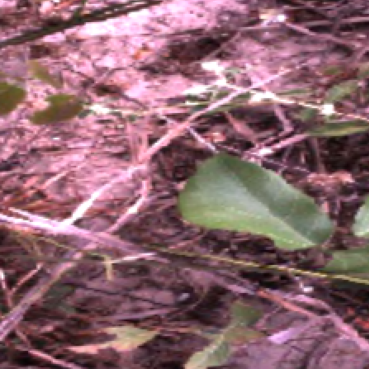
\includegraphics[width=\textwidth]{figuras/implementacion/dataset/imagenes_datagen_1.png}
        \caption{}
    \end{subfigure}
    \hfill
    \begin{subfigure}{0.3\textwidth}
        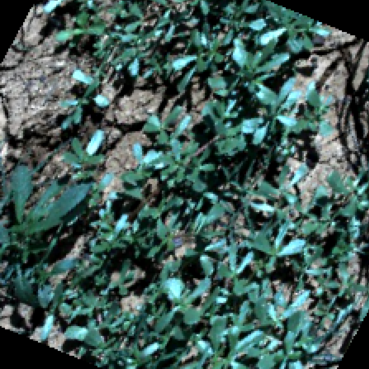
\includegraphics[width=\textwidth]{figuras/implementacion/dataset/imagenes_datagen_2.png}
        \caption{}
    \end{subfigure}
    \hfill
    \begin{subfigure}{0.3\textwidth}
        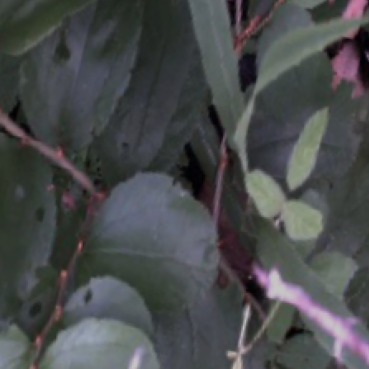
\includegraphics[width=\textwidth]{figuras/implementacion/dataset/imagenes_datagen_3.png}
        \caption{}
    \end{subfigure}
    \hfill
    \begin{subfigure}{0.3\textwidth}
        \includegraphics[width=\textwidth]{figuras/implementacion/dataset/imagenes_datagen_4.png}
        \caption{}
    \end{subfigure}
    \hfill
    \begin{subfigure}{0.3\textwidth}
        \includegraphics[width=\textwidth]{figuras/implementacion/dataset/imagenes_datagen_5.png}
        \caption{}
    \end{subfigure}
    \hfill
    \begin{subfigure}{0.3\textwidth}
        \includegraphics[width=\textwidth]{figuras/implementacion/dataset/imagenes_datagen_6.png}
        \caption{}
    \end{subfigure}
    \caption{Ejemplo de aplicación de \textit{Data Augmentation} a algunas imágenes del \textit{dataset}}
    \label{fig:datagen}
\end{figure}

\subsection{Capas Completamente Conectadas (\textit{Fully Connected Layers})}

Tras la generación de la arquitectura de la red, aún esta no está completa, ya que no tiene la capacidad de convertir la información extraída de las imágenes en las etiquetas en las que van a ser clasificadas. Por esto, se ha de añadir finalmente una estructura que sea capaz de pasar de los datos extraídos a las etiquetas de la imágenes dadas.

En este caso, se ha seleccionado la adición final de una \textbf{capa completamente conectada densa}, que tendrá el tamaño de salida del número de etiquetas de las imágenes a clasificar. Esta seguirá una función de activación \textit{softmax}, la cual normalizará la salida a una distribución de probabilidad a lo largo de las diferentes etiquetas.

\subsection{Entrenamiento por Lotes (\textit{Batch Training})}

Para la implementación realizada, se ha decidido que el entrenamiento siga un entrenamiento por lotes \cite{batch_training_edward}, el cuál está bastante estandarizado en el entrenamiento de redes neuronales. Esto es así, debido a que entrenar con conjuntos de datos completos, requiere gran cantidad de memoria, que en mucho de los casos, es imposible conseguirse. Para ello lo que se hace es entrenar con conjunto de datos más pequeños organizados en lotes en cada tiempo, lo que ocupa menor cantidad de memoria, pero también, entrena en cada tiempo con menor cantidad de datos.

El realizar este tipo de entrenamientos tiene consecuencias en función del tamaño de lote seleccionado. Un lote más pequeño, es más ruidoso, por lo que la red generaliza de peor forma. Por otro lado, un tamaño de lote más grande, tiene mayor capacidad de generalización \cite{brownlee_how_2019}.

Otra consecuencia, es el tiempo por \textit{epoch}, que para lotes más grandes, se ve reducido este tiempo de manera considerable, lo cual es adecuado para la aplicación que se está buscando, donde una pequeña diferencia temporal, finalmente pueden supone varias horas de reducción total. Es por ello, que habiendo ajustado bien el resto de parámetros, se buscará tener lotes altos \cite{chang_effect_2020}.

En este caso, se tiene bastante memoria dedicada al entrenamiento de las redes, pero no es suficiente para almacenar el \textit{dataset} completo. Es por ello que realizando diferentes pruebas del lote más alto que puede ejecutar la red, se establece que el lote con el que se entrenará es de \textbf{32} imágenes.

\subsection{Métodos de Descenso de Gradiente}

Dentro de la implementación del algoritmo del Descenso del Gradiente, existen diferentes formas de mejorar el rendimiento de este, en función del entrenamiento, persiguiendo localizar de forma eficiente y rápida los mínimos globales, evitando el estancarse en mínimos locales.

Para esto, Tensorflow facilita la implementación de diferentes técnicas que pueden ser empleadas en este caso. Las más empleadas son: \textit{Stochastic Gradient Descent} (SGD), Momentum, AdaGrad, RMSProp y Adam. A continuación, se va a realizar una rápida explicación de cada uno de estos métodos.

\begin{itemize}
    \item \textbf{SGD:} El funcionamiento básico es el ya explicado en las bases teóricas, y se basa simplemente en desplazarse en dirección contraria al gradiente de forma proporcional a este y a un \textit{learn rate} seleccionado \cite{NIPS2010_abea47ba}, al que se le añade cierta oscilación, con el que tratar de evitar el estancarse en ciertos mínimos locales, y aumentar la exploración a largo del espacio de búsqueda. Este tiene ciertos problemas cuando el los pasos del gradiente son diferentes entre las distintas dimensiones del espacio de búsqueda, ya que las oscilaciones pueden ser demasiado grandes.
    
    \item \textbf{Momentum:} Este añade la idea basada en la adición de cierta inercia al desplazamiento original del descenso de gradiente \cite{QIAN1999145}, para evitar los problemas que trae SDG. Esto hace que, debido a la velocidad acumulada en el descenso del gradiente, disminuya las oscilaciones de forma adecuada hacía la dirección del gradiente, haciendo que a la vez, se llegue de forma más rápida al mínimo.
    
    \item \textbf{AdaGrad:} A diferencia de los anteriores, este método adapta el \textit{learn rate} a cada uno de los parámetros de la red, haciendo que sea más grande el \textit{learn rate} para parámetros que se modifican en menos ocasiones y más pequeños para los que lo hacen más frecuentemente \cite{JMLR:v12:duchi11a}. Esto aumenta la robustez de la búsqueda frente a los métodos anteriormente comentados. 
    
    \item \textbf{RMSProp:} Este es una variación de AdaGrad, en el cual en vez tener acumulados todos los gradientes, se añade el concepto de la variable ``w'', la cual fija una ventana, considerando únicamente los gradientes más recientes \cite{hinton_srivastava_swersky}. Este soluciona los problemas que tiene AdaGrad, que en tiempos avanzados los pasos se hacen demasiado pequeños, lo cual hace muy lento el proceso de entrenamiento.
    
    \item \textbf{Adam:} Se trata de una combinación entre RMSProp y Momentum, donde se calcula una combinación lineal entre el gradiente y el incremento anterior, además de considerar los gradientes recientemente aparecidos para mantener diferentes tasas de aprendizaje para cada una de los parámetros de la red \cite{kingma2017adam}.
    
\end{itemize}

Una vez conocidas las cualidades \cite{DBLP:journals/corr/Ruder16} y desempeño \cite{jiang_visual_2020} de cada una de estas, y por tanto se selecciona la implementación de \textbf{Adam}, ya que este es el más extendido en la actualidad y se considera que es el adecuado para el entrenamiento de las numerosas arquitecturas que van a ir apareciendo, ya que es el que da un mejor rendimiento en términos generales a otros tipos de métodos estudiados.

\subsection{Métricas de \textit{Accuracy} y \textit{Loss}}

Para una correcta evaluación del desempeño de la red, es importante seleccionar las métricas que medirán los valores de \textit{accuracy} y \textit{loss} de la red. Existen diferentes formas de evaluarse estas, en función de que problema se esté tratando de resolver con el clasificador en cuestión \cite{dommaraju_keras_2020}.

El problema que de clasificación que se está resolviendo en este caso, es un problema multi-clase. Esto significa que se tienen más de dos clases o etiquetas a clasificar, pero que solo una de ellas se corresponderá al mismo tiempo en la imagen de entrada. Por lo tanto, no aparecerán diferentes tipos de malas hierbas en la misma imagen, sino que solo aparecerá una planta en cada imagen.

Para este tipo de problemas, se emplea el denominado \textbf{\textit{categorical accuracy}}, el cual establece cuantas imágenes se han clasificado de forma correcta del total de imágenes de esta categoría a clasificar.

Para evaluar el \textit{loss}, se va a emplear el denominado \textbf{\textit{cross-entropy loss}}, el cual es el adecuado para arquitecturas como las que se van a generar en esta implementación, donde la última capa densa, la función de activación es \textit{softmax}, ya que la red está diseñada para dar una cierta probabilidad a cada una de las etiquetas de ser el tipo de mala hierba de la imagen de entrada.

\subsection{\textit{Learn Rate} Adaptativo}

Durante el entrenamiento de una red neuronal, es posible que el \textit{learn rate}, no sea el adecuado, haciendo que no se llegue a entrenar de forma adecuada. Esto depende mucho de la arquitectura y los datos de entrenamiento, por lo que un valor fijo puede que no sea adecuado. Esto se debe a lo que ya se comentaba en la sección de las bases teóricas, y es que unos valores de \textit{learn rate} demasiado alto provoca que puede que jamás se llegué a optimizar la red a un óptimo e incluso hacer que diverja. Por otro lado un valor demasiado bajo puede hacer que el entrenamiento se haga demasiado largo, tardando mucho en alcanzar el óptimo. En las figuras \ref{fig:learn_rate}, se puede comprobar el comportamiento que se está comentando.

\begin{figure}[h]
\centering
    \begin{subfigure}{0.49\textwidth}
        \centering
        \includegraphics[width=\textwidth]{figuras/implementacion/learn rate bajo.pdf}
        \caption{\textit{Learn Rate} bajo}
        \label{fig:LR_bajo}
    \end{subfigure}
    \hfill
    \begin{subfigure}{0.49\textwidth}
        \centering
        \includegraphics[width=\textwidth]{figuras/implementacion/learn rate alto.pdf}
        \caption{\textit{Learn Rate} alto}
        \label{fig:LR_alto}
    \end{subfigure}
    \hfill
    \begin{subfigure}{0.49\textwidth}
        \centering
        \includegraphics[width=\textwidth]{figuras/implementacion/learn rate optimo.pdf}
        \caption{\textit{Learn Rate} óptimo}
        \label{fig:LR_optimo}
    \end{subfigure}
\caption{Comportamiento en función del \textit{Learn Rate}}
\label{fig:learn_rate}
\end{figure}

Es por esto, que debido a que se tienen que entrenar numerosas arquitecturas diferentes y con diferente requerimiento, se implementa un algoritmo de \textbf{\textit{Learn Rate} adaptativo}. El funcionamiento de este se basa en el establecimiento de un \textit{Learn Rate} inicial alto. Posteriormente se debe monitorizar el error de validación. A partir de la evolución de este parámetro, se conocerá la capacidad de seguir aprendiendo de la red. Si este deja de disminuir en cierto punto, quiere decir que el \textit{Learn Rate} es demasiado alto o ha llegado a un punto óptimo. Para ello se establece un valor de \textit{paciencia}, por el cual, si el error de validación no ha disminuido en cierta cantidad de \textit{epochs}, se divide el valor de \textit{learn rate} entre dos. Así hasta que el entrenamiento haya concluido.

\subsection{Condición de parada}

Por la misma razón que se debe introducir un \textit{learn rate} adaptativo, debe establecerse una condición de parada de entrenamiento que sea variable en función de la arquitectura de la red, ya que cada una requiere mayor o menor tiempo de entrenamiento en función de sus características. Es por ello que se introduce el \textbf{\textit{Early Stopping}} \cite{Prechelt1998} dentro de la implementación realizada.

El funcionamiento de este es similar a lo que ya se veía en el \textit{Learn Rate} adaptativo. Se debe monitorizar una variable a lo largo del entrenamiento y se establece un valor de \textit{paciencia}. Esta variable ha de estar disminuyendo durante los \textit{epochs} establecidos en el valor de paciencia. Si no ha disminuido en este valor de \textit{epochs} establecido se termina el entrenamiento.

De igual manera, en este caso se va a monitorizar el error de validación durante el entrenamiento, que como ya se comentaba anteriormente, nos indica la capacidad de seguir aprendiendo que tiene la red. Además, es una forma de detectar el punto donde la red está comenzando a realizar \textit{overfitting}.

\subsection{Resolución de la Imagen de Entrada}

Debido a las limitaciones computacionales que se han resaltado durante todo el trabajo, es necesario encontrar formas de ejecutar el código de forma eficiente. Es por ello que, para agilizar el entrenamiento de las redes, se ha optado por entrenarse con imágenes de menor resolución. Esto agiliza en varios ordenes de magnitud los tiempos de entrenamiento de las redes, lo cuál permite la ejecución de este algoritmo en tiempos que hace interesante su uso en aplicaciones reales.

Esto tiene contrapartidas, y es la pérdida de información valiosa de las imágenes para su clasificación debido a la bajada de resolución de las mismas. Para ello durante la experimentación, se verificará cual es la resolución adecuada para la ejecución del Algoritmo Evolutivo, de manera que en tiempos adecuados se pueda verificar el desempeños de las diferentes arquitecturas y compararlas entre sí. 

\subsection{Entrenamiento manual posterior de los mejores individuos}

Debido a lo comentado en el apartado anterior, las redes durante la ejecución del Algoritmo Genético, se entrenan con imágenes de menor resolución. Esto nos permite descubrir arquitecturas con gran desempeño o posible potencial para clasificar las imágenes de entrada.

Esto no resulta el entrenamiento final de la red, sino que para esta se le establecen requisitos mayores, y por tanto, se debe extraer el mayor potencial de las redes. Es por ello que deben ser entrenadas posteriormente con mayor delicadeza y conciencia para que estas rindan de la mejor manera posible.

Para esto se establecen mayores tiempo de entrenamiento y condiciones de paradas más extensas. Además, la resolución de entrada de las imágenes serán de mayor tamaño, ya que las limitaciones temporales y computacionales, no son tan grandes como en las que se podrían requerir durante la ejecución del Algoritmo Genético.

Durante la experimentación se tratará de verificar que este procedimiento es adecuado, y que con entrenamientos más largos y con imágenes de entrada de mayor resolución, el desempeño de las redes crece de manera considerable, y por tanto, se extrae el potencial completo de las arquitecturas generadas.
  % INCLUDE: implementación
% !TEX root = ../my-thesis.tex
%
\chapter{EXPERIMENTACIÓN Y RESULTADOS}
\label{sec:resultados}

A lo largo de este capítulo, se mostrarán y explicarán los diferentes experimentos que han sido necesarios realizar durante la elaboración de este trabajo. También se realizará una discusión sobre los resultados, comprobando si las hipótesis inicialmente formuladas son verificadas.

\section{Entorno de ejecución}
El entorno de ejecución y trabajo empleados para el desarrollo de las pruebas realizadas es un punto totalmente vital para la correcta elaboración de este trabajo. Esto es debido a la naturaleza del propio trabajo, el cuál tiene como objetivo el resolver un problema con un requerimiento computacional muy alto.

El entrenamiento de Redes Neuronales es un problema de optimización intrínsecamente paralelo. Es por esto que es de gran importancia el contar con un hardware de trabajo adecuado.

En los últimos años, se ha comprobado como las \textbf{GPUs} (\textit{Graphics Processing Units}) han sido clave para la rápida escalada de estos algoritmos en el uso y resolución normal de problemas. Esto es debido a lo que anteriormente se comentaba, y es que la arquitectura intrínseca de las mismas permiten un gran avance en el procesamiento y el cálculo en paralelo, justo al contrario de lo que sucede con las habituales \textbf{CPUs} (\textit{Central Processing Units}).

Debido a todo esto, un punto totalmente vital de este trabajo es la capacidad computacional de la que se tiene disponible para la realización de esta experimentación, ya que se necesitan de máquinas preparadas específicamente para este tipo de propósitos. Esta nos debe dar facilidades y herramientas para la ejecución de programas de gran tiempo de ejecución y con diferentes configuraciones.

Por todo lo anterior comentado resulta imposible la ejecución de estos programas en un ordenador tradicional, por lo que se requerirá la búsqueda y prueba de grandes infraestructuras de computación preparados para el desarrollo de este tipo de tecnologías. Estas disponen de hardware especializado para estos desarrollos y se ponen a disponibilidad de la comunidad investigadora para su uso.

Debido a que estas son compartidas, contarán con diferentes limitaciones para no monopolizar el uso de las mismas, por lo que se tendrán limitaciones temporales de ejecución, de horas totales, de prioridad y de solicitud de hardware disponible. Es por ello que el conocimiento de estas limitaciones y la adaptación a ellas son totalmente necesarias para la adecuada ejecución de los programas.

Los largos tiempos de ejecución necesarios para el lanzamiento de diferentes topologías de redes convolucionales y su entrenamiento lleva a ingeniarse diferentes soluciones para disminuir el tiempo de cómputo de forma eficiente, como se verán en próximos capítulos.

\subsection{Artemisa}
\textbf{Artemisa} (\textit{ARTificial Environment for ML and Innovation in Scientific Advanced Computing}) \footnote{\url{https://artemisa.ific.uv.es/web/}} es la infraestructura de computación dedicada a inteligencia artificial desarrollada por el \textbf{IFIC} (\textit{Instituto de Física Corpuscular}) asociado al \textbf{CSIC} y a la \textit{Universitat de València}.

Esta plataforma de computación esta dedicada a técnicas de Inteligencia Artificial como \textit{Machine Learning} y \textit{Big Data}. Esta se desarrolla a partir del centro de cálculo del IFIC, la cual dentro del \textit{Programa operativo FEDER de la Comunitat Valenciana 2014-2020} aportó la financiación necesaria para la adquisición de la infraestructura y equipamiento. Este alberga dentro de uno de sus nodos dedicados a la red de computación (\textit{Grid}) los datos obtenidos por el experimento ATLAS del LHC entre otros experimentos. 

En la figura \ref{fig:artemisa}, se puede ver una fotografía de como es físicamente una parte de esta plataforma de computación.

\begin{figure}[ht]
    \centering
    \includegraphics[width=1.0\textwidth]{figuras/centro_calculo_ific.jpg}
    \caption{Fotografía de la plataforma de computación Artemisa}
    \label{fig:artemisa}
\end{figure}

Artemisa dispone de un sistema de cálculo de altas prestaciones multi-GPU para el desarrollo de aplicaciones basadas en Inteligencia Artificial. Cuenta actualmente con 23 servidores que alojan varias tarjetas gráficas especialmente desarrolladas para el cálculo en Inteligencia Artificial, que van a ser usados en modo \textit{batch} y donde podemos encontrar varias interfaces. Además de esto, Artemisa cuenta con CPUs de última generación y con sistemas de almacenamiento de gran velocidad.

Artemisa se desarrolla bajo el sistema operativo de \textit{Linux Centos 7}, que se trata de una distribución libre basada en \textit{Red Hat Enterprise Linux (RHEL) 7}. Además trae instalado numerosas herramientas que son de utilidad para el lanzamiento y ejecución de programas. En el caso de este trabajo, destacar \textit{Python 3.6.1}, el uso de los \textit{Containers} de \textit{Dockers} y los \textit{Virtual Environment} de \textit{Python}.

\subsection{Hardware}
Dada a la importancia del hardware de este para la ejecución de nuestros programas presentaremos cuales están instalados en Artemisa ya que a más potente o mejor preparado este para nuestro problema, más rápidamente y eficientemente se realizarán las ejecuciones.

El hardware de Artemisa se estructura en nodos de tres clases diferentes:
\begin{itemize}
    \item \textbf{Interfaces de Usuario (UI):} es el punto de entrada del usuario, facilitando un entorno de trabajo donde compilar y probar sus programas. Cuando un \textit{job} esta disponible, los usuarios pueden subir desde aquí los diferentes paquetes de trabajo con el \textit{Job Management System} a los \textit{Nodos de Trabajo}
    \item \textbf{Nodos de Trabajo (WN):} donde los usuarios pueden ejecutar sus paquetes de trabajo. Contiene CPUs de gran potencia, gran cantidad de memoria y 4 \textit{GPGPU} de gran velocidad.
    \item \textbf{Nodos de Almacenamiento:} son servidores donde el usuario puede almacenar sus datos y los datos de sus proyectos, y son accesibles tanto por las \textit{Interfaces de Usuario} como por los \textit{Nodos de Trabajo}.
\end{itemize}

A continuación se presenta el hardware del que está compuesto Artemisa:

\begin{itemize}
    \item 2 Interfaces de Usuario (mlui01.ific.uv.es, mlui02.ific.uv.es) con:
    \begin{itemize}
        \item 2 x Intel Xeon Gold 6130 CPU @ 2.10GHz 16c
        \item 192 GBytes ECC DDR4 a 2666 MHz
        \item 1 x GPU Tesla Pascal P100 PCIe
    \end{itemize}
    \item 2 x Nodos de Trabajo con:
    \begin{itemize}
        \item 2 x Intel Xeon Platinum 8160 CPU @ 2.10GHz 24c
        \item 384 GBytes ECC DDR4 a 2666 MHz
        \item 1 x GPU Tesla Volta V100 PCIe
    \end{itemize}
    \item 20 x Nodos de Trabajo con:
    \begin{itemize}
        \item 2 x Intel(R) Xeon(R) Gold 6248 CPU @ 2.50GHz 20c
        \item 384 GBytes ECC DDR4 a 2933 MHz
        \item 1 x GPU Tesla Volta V100 PCIe
    \end{itemize}
    \item 1 x Nodos de Trabajo con:
    \begin{itemize}
        \item 2 x Intel Xeon Platinum 8180 CPU @ 2.50GHz 28c
        \item 768 GBytes ECC DDR4 s 2666 MHz
        \item 4 x GPU Tesla Volta V100 SMX2
    \end{itemize}
    \item 5 x Servidores de Almacenamiento con:
    \begin{itemize}
        \item 2 x Intel Xeon Gold 6130 CPU @ 2.10GH 16c
        \item 192 GBytes ECC DDR4 a 2666 MHz
        \item 6 x 8TB SAS 12 Ggb/s SEAGATE ST8000NM0065
    \end{itemize}
\end{itemize}

Además de esto, su conexión es de vital importancia, ya que a estos dispositivos el acceso se hace de forma totalmente remota, es por ello que se cuenta con conexión \textbf{Ethernet de 10 Gbps} dentro de toda la instalación.

\subsection{HTCondor}
Artemisa necesita una administración eficiente del hardware disponible (\textit{Job Management System}), ya que sino de otra forma se estaría desperdiciando todo su potencial. Es por ello que este integra el software de \textbf{HTCondor} \footnote{\url{https://research.cs.wisc.edu/htcondor/}}. Este permite la creación de un entorno de computación de alto rendimiento (HTC). Además ayuda a extraer eficazmente la potencia informática de las diferentes máquinas conectadas en la red. Esto viene dado debido al desarrollo en el provecho de recursos compartidos con la propiedad distribuida.

Para trabajar con este, como usuario, se ha de enviar los diferentes trabajos a HTCondor. Este es capaz de localizar las máquinas disponibles y ejecuta los trabajos allí. Además, en caso de fallo de una de las máquinas, HTCondor gestionará su ejecución en otra que este disponible de forma automatizada.

Por parte del usuario, facilita en gran medida ejecutar diferentes instancias de un mismo programa de manera sencilla durante largo tiempo de ejecución, despreocupándose de problemáticas que puedan ir apareciendo. Aún así, permite la configuración del lanzamiento de su código, solicitando una cantidad mínima de hardware necesario para la correcta ejecución, que este software lo administrará para hacerlo de forma adecuada.

Debido a que el uso de Artemisa es compartido por varios usuarios, HTCondor es capaz de administrar el hardware y poner limitaciones a cada uno de ellos, evitando monopolizar el tiempo y la potencia de esta infraestructura. Es por ello que puede priorizar diferentes trabajos a usuarios que hayan realizado menor tiempo de ejecución en el sistema.

Artemisa cuenta con varias limitaciones para asegurar el reparto equitativo del uso de la herramienta. Es por ello, que el desarrollo del programa de ejecución debe estar en la línea de estas limitaciones, para tratar de que afecten a su ejecución lo menos posible. Algunas de estas limitaciones son:

\begin{itemize}
    \item Máximo tiempo de ejecución: 48 horas
    \item Máximos \textit{Cores} disponibles: 8
    \item Máxima memoria disponible: 32768 MB
    \item Máximas GPUs disponibles: 4
\end{itemize}

Teniendo en cuenta estas limitaciones, se ha tenido que desarrollar una serie de adaptaciones al código a partir de la generación de \textit{Checkpoints} para la ejecución de programas durante tiempos superiores a 48 horas. De esta manera se puede retomar ejecuciones de programas exactamente por el punto donde se había quedado anteriormente, lo que flexibiliza y facilita mucho la investigación acerca del área que se está tratando.


\section{Experimentos y Discusión}

En esta sección, se pasarán a verificar diferentes hipótesis que se han ido elaborando a lo largo del desarrollo del trabajo. Para esto, se presentarán diferentes experimentos que consigan abarcar esta verificación y finalmente, se desarrollarán ciertas discusiones alrededor de los resultados obtenidos.

\subsection{Experimento 1. Número de capas máximo de las CNNs}

El número de capas de las CNNs, es un parámetro vital en el proceso de generación del genotipo dentro del Algoritmo Genético y para el posterior desempeño de su fenotipo a la hora de generar la arquitectura de la CNN. Es por ello que una elección de este valor es totalmente esencial para la creación de arquitecturas de CNNs adecuadas para la resolución de clasificación de imágenes.

Se busca que las redes tengan tamaños reducidos, que sean capaces de competir con redes existentes actuales para la clasificación de imágenes. A pesar de esto, un número bajo de capas puede producir una peor resolución de este problema, ya que no son capaces de extraer la cantidad suficiente de características necesarias para clasificar las imágenes de entrada.

Por otro lado, un valor demasiado grande de capas, puede hacer que exista información dentro del genotipo que no se manifieste nunca, ampliando de manera muy amplia el espacio de búsqueda de soluciones. Además, puede llevar de la misma manera a generar redes demasiado lentas de entrenar, que nos desvíen del objetivo propuesto en este trabajo.

Es por esto, que se propone la realización de este experimento, para obtener un número de capas adecuado, donde se puedan generar una gran variedad de estructuras de CNNs suficientemente buenas para obtener un clasificador suficientemente robusto y óptimo para la problema propuesto.

Para esto, se han observado como son los individuos que se generan con un máximo de capas de 10, 12, 14, 16 y 20 en diferentes ejecuciones, viendo como es la evolución de estos a lo largo del tiempo. Posteriormente, se monitoriza cuando el número de capas máximo establecido resulta una limitación para la generación libre del número de capas que tienen los individuos generados.

\begin{table}[h]
\caption{Evolución de los individuos que no se limitan por el número de capas máximo establecidos en los parámetros}
\label{tab:numero_capas}
\centering
\begin{tabular}{l|rrrrr}
\toprule
\textbf{Número de capas máximo}            & 10   & 12   & 14   & 16   & 20   \\ \hline
\textbf{\% de individuos con menos capas} & 65,9 & 84,7 & 93,8 & 94,8 & 99,1\\
\bottomrule
\end{tabular}
\end{table}

En la Tabla \ref{tab:numero_capas}, se puede observar como es la evolución anteriormente comentada, es la esperada, disminuyendo el número de individuos limitados cuanto más grande es el número de capas máximo. Se observa un gran salto a partir del número de capas 14, pasando a ser solo cerca del 6\% de los individuos que se ven limitados. Por tanto, se cree adecuado tomar valores superiores a este, para verificar que esta limitación no perjudica en gran medida las desempeño de las redes generadas.

Aún así, un valor muy a tener en cuenta es el de 20 capas máximo, ya que se puede observar que menos del 1 \% de los individuos se ven restringidos por esta limitación, no siendo muy superiores además los tiempos totales de ejecución del algoritmo.


\subsection{Experimento 2. CNNs generadas con tamaño de entrada a \textit{Fully Connected Layers} demasiado grande}

Hay ocasiones, que debido a la naturaleza de la estructura de la CNN generada, puede que las imágenes procesadas de la última capa no hayan conseguido llegar a un tamaño suficientemente reducido para que posteriormente sea procesado por la capa \textit{Fully Connected} para su clasificación. 

Se sostiene la hipótesis que esto podría llevar a un aumento considerable de los tiempos de procesamiento y que el rendimiento de la red sea bastante menor de lo esperado, si esto sucede. Esto se pensó así, debido a la estructura que tienen las redes neuronales convolucionales más empleadas actualmente, donde como se puede ver en la Tabla \ref{tab:ultima_capa_redes}, el tamaño de las FM en esta última capa, era más o menos constante y comprendido en un rango, por lo que se pensó en considerar como individuos malos los individuos que no siguieran esta forma, descartándolos de la siguiente población.

\begin{table}[h]
\caption{Tamaño de la \textit{Feature Map} en la última capa de las redes más empleadas en la actualidad}
\label{tab:ultima_capa_redes}
\centering
\begin{tabular}{l|c}
\toprule
\textbf{Red Neuronal Convolucional} & \multicolumn{1}{l}{\textbf{Tamaño última capa}} \\ \hline
LeNet \cite{lesnet}                             & 5x5      \\
AlexNet \cite{NIPS2012_c399862d}                            & 6x6  \\
VGG-16 \cite{simonyan2015deep}                             & 7x7 \\
Inception V1 \cite{szegedy2014going}                       & 7x7 \\
Inception V3 \cite{szegedy2015rethinking}                       & 8x8   \\
Resnet-50 \cite{He2016}                          & 7x7                                             \\
Xception \cite{chollet2017xception}                           & 10x10  \\
Inveption V4 \cite{szegedy2016inceptionv4}                       & 8x8 \\
ResnetXT-50 \cite{xie2017aggregated}                        & 7x7      \\
\bottomrule
\end{tabular}
\end{table}

Es por ello, que con este experimento, se pretende investigar si es adecuado descartar estar redes y denominarlas como redes \textit{no válidas} y asignarles un valor de \textit{fitness} igual a cero para que sean descartadas, o por el contrario, intentar obtener un valor de \textit{fitness} tratando de entrenar la red y valorando el material importante que pueda llevar codificada este individuo.

Para esto, se comienza partiendo de una implementación realizada con esta limitación puesta, donde los individuos que no hayan conseguido que su última capa, antes de la \textit{FCL}, reducir el tamaño de la imagen de entrada a un tamaño de las \textit{Feature Maps} de 8x8, serán descartados. Al realizar esta prueba, se descubre como en más del 50\% de generaciones, al menos un individuo es descartado, y por tanto, se limita la propagación de partes de su genotipo que podrían llegar a ser buenas, viéndose finalmente, la existencia de poca diversidad genética dentro de la población.

\begin{figure}[h]
    \centering
    \includegraphics[width=1\textwidth]{figuras/experimentos/fcl_grande/con_limitacion_1.pdf}
    \caption{Muestra de evolución de la implementación con limitación en el tamaño de \textit{FM} a la entrada de la \textit{FCL}}
    \label{fig:con_limit_fcl}
\end{figure}

Esto que se comenta se puede ver claramente en la Figura \ref{fig:con_limit_fcl}, donde se generan gran cantidad de individuos válidos, a lo largo de las diferentes generaciones, haciendo que el algoritmo evolutivo no valore suficientes individuos de forma adecuada. Además, se ve una rápida convergencia del algoritmo a una solución no demasiado buena, con apenas un \textit{fitness} de 0,81 para el mejor individuo en ambas ejecuciones.

En total se lanzaron 8 ejecuciones, consiguiendo resultados equivalentes a las mostradas anteriormente, en todas ellas.

Tras esta apreciación, se ha de comprobar si realmente resulta una limitación real el entrenamiento de estos individuos, que no tienen una forma igual o similar a las arquitecturas encontradas en la literatura. En esto se descubre que lejos de ser una limitación para el Algoritmo Evolutivo, el algoritmo genética funciona de manera más lógica, sin descartar de forma contundente a ninguno de los individuos, y calificando a estos con una \textit{fitness} proporcional a su desempeño en la clasificación de las imágenes de entrada.

\begin{figure}[h]
    \centering
    \includegraphics[width=\textwidth]{figuras/experimentos/fcl_grande/sin_limitacion_1.pdf}
    \caption{Muestra de evolución de la implementación sin limitación en el tamaño de \textit{FM} a la entrada de la \textit{FCL}}
    \label{fig:sin_limit_fcl}
\end{figure}

Esto se observa fácilmente en la Figura \ref{fig:sin_limit_fcl}, donde ya observa que la evolución de los individuos es más lógica, conservando una buena diversidad genética dentro de las diferentes poblaciones. Esto da unos resultados mucho mejores de forma directa, viendo como en estas ejecuciones se obtienen individuos con una \textit{fitness} de hasta 0,88 en una cantidad de generaciones menor, lo que resulta un salto bastante grande en comparación a los individuos obtenidos con la limitación puesta. Este número de generaciones menor puede llegar a ser engañosa ya que en realidad se evalúa una cantidad equivalente de individuos en total, pero se evalúan más individuos en cada generación.

Es por esto, que no se encuentran argumentos de peso para eliminar a ciertos individuos de la evaluación por la forma de su arquitectura, y que todos estos, serán entrenados y se calculará su desempeño en el problema propuesto, asegurando que las partes buenas de este, se propaguen a lo largo de las siguientes generaciones.

\subsection{Experimento 3. Elitismo en Algoritmo Genético}

Al realizarse la implementación del Algoritmo Genético, existen diferentes estrategias que se pueden tomar a la hora de implementar el mismo. Una de ellas es la estrategia de elitismo, como ya se ha explicado en secciones anteriores del trabajo.

El elitismo tiene propiedades que son realmente beneficiosas para cierto tipo de problemas, y se tiene la hipótesis que este es uno de ellos, donde su implementación puede llegar a ser incluso necesaria para la obtención de buenos resultados.

Para comprobar esto se propone la realización de este experimento, donde se comprueba como es la evolución de la implementación del algoritmo sin implementar la estrategia de elitismo y verificar si sin implementar este, se puede llegar a obtener resultados adecuados, o por otro lado, es necesario el asegurar la conservación de los mejores individuos a lo largo de las diferentes generaciones, evitando que su información genética valiosa se pierda.

Se han lanzado 8 ejecuciones durante un tiempo total de 96 horas de ejecución cada una de ellas y los resultados son los obtenidos en la figura \ref{fig:exp_elitismo}.

\begin{figure}
\centering
    \begin{subfigure}{1\textwidth}
        \centering
        \includegraphics[width=\textwidth]{figuras/experimentos/exp_no_elitismo/legend.pdf}
    \end{subfigure}
    \begin{subfigure}{0.47\textwidth}
        \centering
        \includegraphics[width=\textwidth]{figuras/experimentos/exp_no_elitismo/no_elitismo_0.pdf}
        \caption{Ejecución 0}
    \end{subfigure}
    \hfill
    \begin{subfigure}{0.47\textwidth}
        \centering
        \includegraphics[width=\textwidth]{figuras/experimentos/exp_no_elitismo/no_elitismo_1.pdf}
        \caption{Ejecución 1}
    \end{subfigure}
    \hfill
    \begin{subfigure}{0.47\textwidth}
        \centering
        \includegraphics[width=\textwidth]{figuras/experimentos/exp_no_elitismo/no_elitismo_2.pdf}
        \caption{Ejecución 2}
    \end{subfigure}
    \hfill
    \begin{subfigure}{0.47\textwidth}
        \centering
        \includegraphics[width=\textwidth]{figuras/experimentos/exp_no_elitismo/no_elitismo_3.pdf}
        \caption{Ejecución 3}
    \end{subfigure}
    \hfill
    \begin{subfigure}{0.47\textwidth}
        \centering
        \includegraphics[width=\textwidth]{figuras/experimentos/exp_no_elitismo/no_elitismo_4.pdf}
        \caption{Ejecución 4}
    \end{subfigure}
    \hfill
    \begin{subfigure}{0.47\textwidth}
        \centering
        \includegraphics[width=\textwidth]{figuras/experimentos/exp_no_elitismo/no_elitismo_5.pdf}
        \caption{Ejecución 5}
    \end{subfigure}
    \hfill
    \begin{subfigure}{0.47\textwidth}
        \centering
        \includegraphics[width=\textwidth]{figuras/experimentos/exp_no_elitismo/no_elitismo_6.pdf}
        \caption{Ejecución 6}
    \end{subfigure}
    \hfill
    \begin{subfigure}{0.47\textwidth}
        \centering
        \includegraphics[width=\textwidth]{figuras/experimentos/exp_no_elitismo/no_elitismo_7.pdf}
        \caption{Ejecución 7}
    \end{subfigure}
    \hfill
\caption{Resultados del experimento 3, con la eliminación de la estrategia de elitismo}
\label{fig:exp_elitismo}
\end{figure}

Se puede observar que en las 8 ejecuciones, difícilmente se puede apreciar una mejora sustancial del \textit{fitness} a lo largo de las generaciones, y no consiguiendo una cierta progresión deseada dentro de los rangos de tiempo de ejecución deseados. Esto puede indicar que la información valiosa de los diferentes individuos se pierde y no se garantiza su conservación a lo largo de la progresión del algoritmo, como ya se sospechaba que podría suceder.

En conclusión, este experimento indica que es interesante la introducción de un mecanismo de elitismo dentro de la implementación realizada para optimizar las arquitecturas de las CNNs generadas. Este mecanismo hay que introducirlo con cierto cuidado, ya que la introducción de números de elitismo muy alto, puede generar una baja diversidad genética dentro de la población de individuos bastante buenos, lo que no siempre es adecuado para la correcta exploración de todo el espacio de búsqueda del algoritmo genético.


\subsection{Experimento 4. Relación entre tiempo de entrenamiento y estructura de una CNN}

Durante el entrenamiento de algunas de las arquitecturas de redes generadas a partir del Algoritmo Genético, se ha podido observar como ciertos modelos, realizaban tiempos de entrenamiento muy dispares entre ellos, siendo algunos demasiado altos. Además, no se observa una relación clara con el valor de desempeño de estas redes. Esto perjudica en gran manera la búsqueda de ciertas redes de pequeño tamaño y gran desempeño, como sugería el trabajo.

Debido a la gran cantidad de factores que pueden afectar a esta ocurrencia, resulta complicado a simple vista ver cuál es la causa del tiempo de entrenamiento tan dispar entre diferentes redes. 

Es por ello, que se cree necesario realizar un estudio de las propiedades de las diferentes redes generadas y los tiempos de entrenamiento de las mismas, para conocer si existe algún tipo de correlación entre las mismas.

Para realizar esto, en primer lugar, se buscó parametrizar las redes neuronales generadas en varías ejecuciones. Esto significa, obtener ciertos valores que caractericen a la red para poder buscar una relación entre las diferentes variables. Las que finalmente se seleccionaron fueron: \textit{Accuracy}, \textit{Loss}, Número de parámetros, Tiempo de entrenamiento por \textit{epoch}, Número de capas totales, Número de capas convolucionales relativas, Número de capas de \textit{Pooling} relativas, Número de capas convolucionales residuales relativas, Número de funciones de activación \textit{tanh} relativas, Número de funciones de activación \textit{ReLU} relativas, Número de capas convolucionales con \textit{stride} 1 relativas, Número de capas convolucionales con \textit{stride} 2 relativas, Número de capas de \textit{Average Pooling} relativas, Número de capas de \textit{Max Pooling} relativas, Número de capas de \textit{Pooling} con \textit{stride} 2, Número de capas de \textit{Pooling} con \textit{stride} 3 y el \textit{stride} total de la red.

Los valores relativos extraídos, van referidos al número total de capas de la red, para evitar el efecto que pueda tener un mayor o menor  número de capas al tiempo de entrenamiento.

Se ha realizado 8 ejecuciones en total durante un tiempo de ejecución de 96 horas. Esto ha resultado en la generación de un total de 1159 individuos diferentes, los cuales servirán para ver la correlación entre las diferentes variables.

Una vez teniendo los individuos, estos han sido analizados de dos formas diferente: a través del Coeficiente de Correlación de Spearman y por la generación de Bosques Aleatorios (\textit{Random Forest}). Ambos son análisis bivariantes, que serán más que suficientes para realizar el análisis que se pretende realizar.

\begin{itemize}
    \item \textbf{Coeficiente de Correlación de Spearman:} \cite{daniel1990applied} Se ha seleccionado esta correlación matemática, ya que es una forma sencilla de observar la posible asociación o interdependencia entre dos variables aleatorias (continuas o discontinuas) de manera sencilla \cite{Mukaka2012}, ya que no requiere de numerosas condiciones a las propias variables como si puede requerirlo coeficientes de correlaciones como Pearson o Kendall, que requieren cosas cosas como que la distribución de la variable aleatoria siga una normal, condición que puede no cumplirse en nuestras variables 
    
    Esta viene definida entre -1 y 1, siendo un valor negativo una correlación inversa y un valor positivo una correlación directa. Cuanto más cercano a sus extremos, más fuerte es la correlación entre el par de variables.
    
    \begin{figure}[h]
        \centering
        \includegraphics[width=\textwidth]{figuras/experimentos/correlacion/spearman_corr.pdf}
        \caption{Correlación de Spearman entre todas la variables que definen la arquitectura de una CNN}
        \label{fig:todas_correlaciones}
    \end{figure}
    
    La correlación entre todas las variables definidas se puede ver en la figura \ref{fig:todas_correlaciones}. En esta, se muestra el valor absoluto del valor del coeficiente de correlación para que se vea de mejor manera la relación entre las variables.
    
    \begin{figure}[h]
        \centering
        \includegraphics[width=\textwidth]{figuras/experimentos/correlacion/spearman_pvalues.pdf}
        \caption{\textit{P-value} entre todas la variables que definen la arquitectura de una CNN}
        \label{fig:p-value}
    \end{figure}
    
    Este valor de correlación siempre ha de ir acompañado de un valor de significancia o \textit{p-value}, que si realmente el valor del coeficiente de correlación tiene algún tipo de sentido. Este valor índica que cuanto más bajo sea, más significación tiene y por lo tanto el coeficiente de correlación está mostrando un valor con cierto sentido. En la figura \ref{fig:p-value}, se puede ver el valor de significancia para cada valor.
    
    Finalmente, atendiendo a los valores que realmente se quieren extraer en este experimento, se muestran en la tabla \ref{tab:correlacion}, la correlación que existe entre todas las variables con respecto a la variable de Tiempo por \textit{epoch}, para descubrir cuál puede ser el causante de que este valor sea tan dispar entre diferentes arquitecturas.
    
    \begin{table}[h]
    \caption{Correlación de Spearman entre las diferentes variables que caracterizan una CNN junto a su valor de significación}
    \label{tab:correlacion}
    \centering
    \begin{tabular}{l|r|r}
    \toprule
    \textbf{Parámetro} & \textbf{Coeficiente de Correlación de Spearman} & \textbf{Significación (\textit{P-value})} \\ \hline
    Loss               & -0,475                                         & 0                                \\
    N Pool Layers      & -0,390                                         & 0                                \\
    N Conv Stride 2    & -0,365                                         & 0                                \\
    Total Stride       & -0,272                                         & 0                                \\
    N Max Pool         & -0,260                                         & 0                                \\
    N Pool Stride 2    & -0,254                                         & 0                                \\
    N Pool Stride 3    & -0,170                                         & 0                                \\
    N Avg Pool         & -0,143                                         & 0                                \\
    N Conv Layers      & 0,079                                          & 0,010                            \\
    N tanh Activation  & 0,117                                          & 0                                \\
    N ReLU Activation  & 0,145                                          & 0                                \\
    N Skip Layers      & 0,201                                          & 0                                \\
    Accuracy           & 0,471                                          & 0                                \\
    N Params           & 0,494                                          & 0                                \\
    N Layers           & 0,578                                          & 0                                \\
    N Conv Stride 1    & 0,652                                          & 0    \\
    \bottomrule
    \end{tabular}
    \end{table}
    
    Se puede observar como existen varios parámetros con una fuerte correlación con el Tiempo por \textit{Epoch}. Además, se puede observar como se puede confiar en gran medida en los valores obtenidos de correlación ya que el valor de significación de todos los valores prácticamente es 0 en todos ellos.
    
    En primer lugar, destacar el número de capas de convolución con \textit{stride} 1, que se puede observar como es el valor más fuertemente correlado con grandes tiempos por \textit{epoch}. Esto tiene bastante sentido, ya que aplicar una convolución con un \textit{stride} debe realizar prácticamente el doble de operaciones que con un \textit{stride} de 2, que como se puede ver en la tabla, de forma más débil, indica que la aparición de este tipo de capa hace que el tiempo por \textit{epoch} se vea reducido.
    
    En segundo lugar, destacar la variable del número de capas, que de igual manera, nos indica a que a un mayor número de capas, más operaciones se ha de realizar durante el entrenamiento, lo que supone un mayor tiempo por \textit{epoch}. De igual manera, y como ya se sospechaba, sucede con el número de parámetros de la red.
    
    Destacar también, en un cuarto lugar el \textit{accuracy}, en el cual puede verse una ligera tendencia a que los valores con mayor tiempo por \textit{epoch} suelan obtener mejores resultados y por tanto clasificar mejor. Esto es de tener en cuenta debido a que en este trabajo se persigue buscar un equilibrio entre la precisión de clasificación y el tamaño de la red, lo cuál puede ser un mal indicativo de que las mejores redes puedan requerir mayor dedicación y tamaño.
    
    
     \item \textbf{\textit{Random Forest:}} \cite{Breiman2001} Este método se basan en el uso de varios árboles de decisiones, que combinados consiguen clasificar, con cierta eficacia, en función de variables dadas varios conjuntos de datos. En este caso se ha tratado de clasificar entre las redes con un Tiempo por \textit{Epoch} mayor a 80 segundos, para ver que cualidades comparten entre ellas y si son fácilmente separables estos dos grupos a partir de los datos dados.
     
     Con esta división, se consigue una precisión de clasificación del \textbf{0,914}, lo cual es un valor bastante alto. Dentro de esto, se ha obtenido el valor de Importancia (\textit{Importance}), que nos muestras que variables han sido más relevantes en la clasificación. Este valor es mayor cuanto mayor haya aportado esta variable a la tarea de clasificación. Este valor obtenido para cada una de las variables se muestra en la tabla \ref{tab:rf_importance}.
     
    \begin{table}[h]
    \caption{Valor de Importancia obtenido a partir de la generación de Bosques Aleatorios para la variable Tiempo por \textit{Epoch}}
    \label{tab:rf_importance}
    \centering
    \begin{tabular}{l|r}
    \toprule
    \textbf{Parámetro} & \textbf{Importancia (\textit{Importance})} \\ \hline
    N Params           & 0,220                             \\
    N Conv Stride 1    & 0,206                             \\
    N Layers           & 0,140                             \\
    Accuracy           & 0,100                             \\
    Loss               & 0,093                             \\
    Total Stride       & 0,061                             \\
    N Conv Stride 2    & 0,042                             \\
    N Pool Stride 3    & 0,037                             \\
    N Pool Layers      & 0,035                             \\
    N Avg Pool         & 0,016                             \\
    N Max Pool         & 0,014                             \\
    N tanh Activation  & 0,012                             \\
    N ReLU Activation  & 0,008                             \\
    N Conv Layers      & 0,007                             \\
    N Skip Layers      & 0,006                             \\
    N Pool Stride 2    & 0,003   \\
    \bottomrule
    \end{tabular}
    \end{table}
    
    Empleando este método, se puede observar como en primer lugar, la variable que toma mayor importancia a la hora de segmentar entre redes más lentas y redes más rápidas, es el número de parámetros. Se puede ver como el árbol generado, toma esta variable como importante para distinguir el tiempo por \textit{epoch} de la red a entrenar.
    
    En segundo lugar, se encuentra la variable del número de capas de convolución con tamaño de \textit{stride} igual a 1. De igual manera que se comentaba anteriormente, es lógico que esta variable se sitúe en posiciones altas de importancia, debido a que el número de operaciones a realizar cambia drásticamente a si el \textit{stride} fuera de 2.
    
    En tercer lugar, se encuentra el número de capas, que de igual manera como se comentaba con el número de parámetros, era una variable que es lógica encontrarse en estos valores tan altos de importancia.
    
    Por último, comentar de igual manera el protagonismo que toma la variable de \textit{accuracy} a la hora de clasificar entre redes más lentas y más rápidas, lo que tiene mucho sentido, ya que redes más lentas puede deberse a una mayor extracción de características de la foto, que ayude a clasificar posteriormente las imágenes de entrada.
     
\end{itemize}

Como se puede observar, los resultados que se extraen de la aplicación de ambos métodos arrojan resultados similares. Esto se puede ver observando cuáles son las cuatro variables en primeras posiciones en ambos métodos, donde se encuentran en ambos casos a las variables: Número de Capas de Convolución con \textit{stride} 1, Número de capas, Número de parámetros y \textit{Accuracy}. Esto es un buen indicador de que la metodología empleada en ambas metodologías es correcta, y que los indicadores extraídos en este experimento son adecuados.

Para concluir, se extrae como enseñanza de este experimento que existen dos parámetros de la red a los que hay que tratar con especial atención para evitar valores demasiados altos de tiempo por \textit{epoch}, que haga que la operación del algoritmo elaborado sea demasiado lenta, no consiguiendo los objetivos finales marcados en el trabajo. Estas variables son: el \textbf{Número de Parámetros}, que se puede controlar de manera relativamente sencilla jugando con el número de \textit{Feature Maps} de las capas de convolución, evitando que sean excesivamente grandes, y el \textbf{Número de Capas}, que es un parámetro a seleccionar a la hora de ejecutar el algoritmo.


\subsection{Experimento 5. Cantidad de \textit{Features Maps} en las capas de convolución}

Se debe determinar un valor adecuado para la cantidad de \textit{Features Maps} que deben tener las capas de convolución de las redes CNNs que se están generando. Estas, como se veía en la implementación del problema, va codificada su cantidad dentro del genotipo de las propias soluciones.

Se ha sospecha que una cantidad demasiado grande de \textit{Features Maps} en las primeras capas convolucionales de la CNNs, donde las imágenes de entrada tienen un tamaño todavía demasiado grandes, puede generar una gran cantidad de parámetros que pueden hacer demasiado lenta a la red a la hora de su entrenamiento. Esto, visto la dificultad computacional del problema, se debería tratar de evitar en lo máximo posible, y sobretodo si tratamos de seguir la premisa de generar redes suficientemente pequeñas para clasificar las imágenes de entrada.

Por otro lado, seleccionar una cantidad demasiado baja de \textit{Features Maps}, podría realizar que las redes generadas, no sean capaces de obtener las suficientes características de las imágenes para que puedan clasificarlas de manera satisfactoria.

Debido a la importancia de este parámetro, se realizó un trabajo de búsqueda del número de \textit{Features Maps} adecuados en la codificación del Algoritmo Genético. Para esto, se han ido probando diferentes opciones de codificaciones, comprobando el número de parámetros totales de las redes que se iban generando, viendo su desempeño final y su velocidad de entrenamiento. Las opciones probadas son tres, y se van a presentar a continuación.

\begin{itemize}
    \item \textbf{Propuesta 1:} En primer lugar, se proponía una codificación compuesta por 11 bits, donde 3 de ellos estarían formados por la codificación del número de \textit{Features Maps}. Esta, seguía la forma ya presentada en la implementación, pero con la diferencia de que permite una codificación de hasta 8 opciones diferentes de cantidad de filtros. Esto hacía que el rango de estos estuviese compuesta por cantidades de: 16, 32, 64, 128, 256, 512, 1024 y 2048.
    
    Los resultados obtenidos de la ejecución de esta, generaba modelos de cerca de 40 millones de parámetros, con tiempos por \textit{epoch} en el entrenamiento de más de 500 segundos, lo cuál hacia imposible evaluar el suficiente número de individuos de forma adecuada, consiguiendo además valores de \textit{accuracy} cercanos a los 0,84 que resultaban no resultaban excesivamente altos, debido a las pocas generaciones que podía llegar a avanzar el Algoritmo Genético, y las estructuras pocos optimizadas que se obtenían.
    
    \item \textbf{Propuesta 2:} Esta, es consecuencia de los malos resultados obtenidos con la primera propuesta, lo que se llevó a proponer una disminución de las cantidades de \textit{Features Maps} que serían empleadas. Por lo tanto, se pasaría a un rango de cantidades de: 2, 4, 8, 16, 32, 64, 128, 256.
    
    Empleando el mismo tiempo de ejecución total, se obtuvieron mejores resultados, obteniendo redes de tamaños menores a los 5 millones de parámetros y con un rendimiento algo superior, llegándose a alcanzar valores de 0,86 de \textit{accuracy}, y habiendo evaluado una mayor cantidad de individuos. 
    
    \item \textbf{Propuesta 3:} Esta es una modificación de la propuesta 2, donde ve como cantidades menores a 32 filtros por capa de convolución, eran valores demasiados bajos de filtros, y carecía de sentido evaluar este tipo de soluciones. Es por ello que se propone una solución basada en una codificación en 10 bits, donde tan solo 2, se dedican a la codificación del número de \textit{Features Maps}. Esto deja el rango de cantidades de filtros en: 32, 64, 128 y 256. 
    
    De esta manera se llega a la implementación actual, la cuál ha cuál ha sido capaz de obtener individuos cuyos individuos más grandes, tienen tiempos por \textbf{epoch} de cerca de los 200 segundos, lo cuál significa una reducción significativa en el tiempo total de entrenamiento, y además, sin reducir el desempeño obtenido por estas redes.
\end{itemize}

Vistas las experimentaciones y los resultados obtenidos, resulta lógico entender porque se ha mantenido la propuesta 3, como implementación actual del algoritmo para la búsqueda de buenos individuos para la clasificación de imágenes, consiguiendo tiempos de entrenamiento más bajos a los que se podrían obtener inicialmente, sin renunciar al desempeño de estas.

\subsection{Experimento 6. Relación entre la resolución de la imagen de entrada y desempeño de la red}

Para la implementación del Algoritmo Genético propuesto, se puede observar como se ha optado por usar unas imágenes de entrada de menor resolución para el entrenamiento de las diferentes redes neuronales convolucionales generadas, para tratar de reducir el tiempo de entrenamiento. Esto es así, debido al gran requerimiento computacional que se ha visto que tiene la ejecución de este programa.

Esto se ha realizado así, debido a que se tiene la hipótesis de que la resolución de la imagen de entrada no es determinante para la comparación del desempeño en la aplicación de clasificación de los diferentes individuos. Aún así, se debe comprobar que la resolución de entrada de las imágenes y la pérdida de información consecuente de la reducción de las mismas, no es un factor determinante a la hora de valorar la calidad de las estructuras construidas a partir del Algoritmo Genético.

Por otro lado, se pretende comprobar si posteriormente, tomando estas redes generadas a partir del Algoritmo Genético y entrenándolas nuevamente, pero esta vez con imágenes de mayor resolución, siguen manteniendo su capacidad de clasificar de forma adecuada estas imágenes e incluso de hacerlo mejor debido a la mayor cantidad de información que se ha recuperado al aumentar la resolución de la imagen.

\begin{table}[h]
\caption{Individuos seleccionados para el Experimento 6}
\label{tab:mejores_ind_exp6}
\centering
\begin{tabular}{r|r|r}
\toprule
\multicolumn{1}{c|}{\textbf{Id}} & \multicolumn{1}{c|}{\textbf{Genotipo}}                        & \multicolumn{1}{c}{\textbf{Parámetros}} \\ \hline
0                                & (534, 778, 884, 862, 281, 952, 708, 439)                      & 1587907                                      \\
1                                & (852, 990, 983, 914, 328, 679, 944, 307, 1018)                & 885441                                      \\
2                                & (842, 320, 542, 843, 358, 875, 569, 345, 824, 973, 980, 946)  & 498563                                      \\
3                                & (788, 888, 992, 926, 840, 606, 325, 904, 809, 594, 461)       & 1181283                                     \\
4                                & (948, 956, 788, 655, 344, 862, 547, 616, 824)                 & 1071907                                      \\
5                                & (642, 956, 910, 851, 585, 1002, 844, 268, 615, 885, 913, 398) & 1701283                                      \\
6                                & (835, 776, 938, 331, 786, 632, 725, 871, 475)                 & 766755                                      \\
7                                & (590, 1020, 774, 955, 997, 336, 646, 652, 671, 708, 933)      & 4930371   \\
\bottomrule
\end{tabular}
\end{table}

Para esto, se han seleccionado los mejores individuos generados hasta ese momento del experimento, que han sido generados con una cantidad máxima de capas de 15 con la ejecución del Algoritmo Genético en 8 lanzamientos diferentes durante 96 horas en total. Estos son los que aparecen en la Tabla \ref{tab:mejores_ind_exp6}. En esta tabla aparece un identificador del individuo, su genotipo donde cada capa se representa por el número entero que equivale a la cadena de \textit{bits} que la codifica y el número de parámetros de la red.

Durante este experimento, se va a realizar un entrenamiento con imágenes de diferentes tamaños de imagen. Se va a realizar la prueba de entrenamiento con redes de 64x64, 112x112 y de 224x224, siendo este último el tamaño nativo de estas imágenes. 

\begin{table}[h]
\caption{Resultados del entrenamiento de las diferentes redes en función del tamaño de las imágenes de entrada}
\label{tab:resultados_exp6}
\centering
\begin{tabular}{r|rrr|rrr}
\toprule
\multicolumn{1}{c|}{\textbf{Id}} & \multicolumn{3}{c|}{\textbf{Tiempo por \textit{epoch} (s)}}                                              & \multicolumn{3}{c}{\textbf{\textit{Accuracy}}}                                                          \\
\multicolumn{1}{c|}{}   & \multicolumn{1}{c}{\textbf{64x64}} & \multicolumn{1}{c}{\textbf{112x112}} & \multicolumn{1}{c|}{\textbf{224x224}} & \multicolumn{1}{c}{\textbf{64x64}} & \multicolumn{1}{c}{\textbf{112x112}} & \multicolumn{1}{c}{\textbf{224x224}} \\ \hline
0                       & 97                        & 240                         & 875                          & 0,874                     & 0,902                       & x                           \\
1                       & 67                        & 170                         & 623                          & 0,878                     & 0,896                       & 0.886                       \\
2                       & 22                        & 40                          & 135                          & 0,873                     & 0,89                        & 0.882                       \\
3                       & 165                       & 400                         & 1511                         & 0,866                     & 0,905                       & x                           \\
4                       & 57                        & 140                         & 533                          & 0,88                      & 0,922                       & 0.919                       \\
5                       & 84                        & 228                         & 792                          & 0,864                     & 0,897                       & 0.928                       \\
6                       & 26                        & 52                          & 169                          & 0,86                      & 0,898                       & 0.916                       \\
7                       & 215                       & 566                         & 2221                         & 0,868                     & 0,898                       & x  \\
\bottomrule
\end{tabular}
\end{table}

En la Tabla \ref{tab:resultados_exp6}, se puede ver el resultado de entrenar estas redes, ante parámetros de entrenamiento iguales, con \textit{patience} del \textit{Early Stopping} de 32, \textit{patience} del \textit{Learning Rate} Adaptativo de 16 y con \textit{Learn Rate} inicial de 0,001. Se puede observar como debido a los altos tiempos de entrenamiento de algunas de las redes, en el entrenamiento de las redes para imágenes de tamaño 224x224, no ha sido posible completarse en un tiempo inferior a 48 horas.

Se puede observar como la tendencia del desempeño de estas redes es creciente con el tamaño de las imágenes de entrada, viéndose una mejora drástica en el salto a las imágenes de 112x122, consiguiendo obtener hasta un desempeño del 0,922 por el cuarto individuo. El salto posterior a imágenes de 224x224, la mejora no es tan significativa, si siendo el salto en el tiempo de entrenamiento bastante superior, llegando a ser hasta 10 veces mayor que para imágenes de tamaño 64x64.

Además, se puede observar como aún habiendo mejorado todas las redes, el desempeño entre las redes a igual tamaño de imagen de entrada, sigue manteniéndose de forma similar, manteniéndose el mejor individuo sobre el resto.

Esto es una gran noticia, ya que se puede observar con estos resultados que la hipótesis realizada inicialmente, se puede considerar cierta, ya que las redes, a pesar de haber sido seleccionadas para imágenes de entradas menores, tienen capacidad de mejora con imágenes de entrada de menor tamaño. Esto permite realizar el proceso de ejecución del Algoritmo Genético empleando imágenes más pequeñas, que agilicen la localización de las mejores arquitecturas de forma más rápida. Posteriormente, estas pueden ser entrenadas con imágenes más grandes y usadas para clasificar imágenes del tamaño nativo, sabiendo que si este individuo ha tenido un buen desempeño con imágenes pequeñas, lo hará de igual o mejor manera con imágenes de tamaños más grandes.

\subsection{Experimento 7. Parámetros de entrenamiento de las CNNs para la ejecución del Algoritmo Genético}

El entrenamiento de las redes, es algo que debe ser establecido al inicio de la implementación de la solución, ya que es algo que afecta posteriormente a comprobar el rendimiento de cada uno de las arquitecturas generadas. Además, es el gran cuello de botella de la ejecución del algoritmo genético, ya que conlleva el mayor peso computacional de la implementación.

Por todo lo comentado, es muy importante establecer un marco genérico suficientemente flexible para dar la oportunidad a todos los individuos a entrenar hasta una capacidad adecuada, que permita establecer un marco de comparación justo entre ellos.

Para esto, como se comenta en la implementación, se establecen varias estrategias que permiten flexibilizar el entrenamiento a la capacidad de seguir aprendiendo a las diferentes CNNs, evitando a su vez el indeseado efecto del \textit{overfitting}. Estas estrategias son el \textit{Early Stopping} y el \textit{Learn Rate} Adaptativo. Estos tienen dos parámetros claves que han de ser ajustados de manera que el rendimiento sea adecuado en todas las condiciones, asegurando que la comparación entre las diferentes redes es justa.

Además existe otro tercer parámetro que debe ser seleccionado, que es el \textit{learn rate} inicial, con el que se comenzará a entrenar a la red. La selección de un valor inadecuado, haría que el conjunto de las redes probadas, no diera valores significativos de las capacidades reales de los individuos.

Para la realización de estas pruebas, se tomarán a los individuos ya presentados en el Experimento 6, que están recogidos en la Tabla \ref{tab:mejores_ind_exp6}, los cuáles serán entrenados con diferentes configuraciones para comprobar su desempeño.

En primer lugar, se va a realizar una comprobación del \textit{learn rate} inicial adecuado, que simplemente este ha de ser suficientemente alto para que el entrenamiento se haga de forma adecuada, ya que será ajustado en función de las necesidades por el optimizador y por la programación del \textit{Learn Rate} Adaptativo. Para esto, se han probado dos valores bastante genéricos y altos de este parámetro para comprobar cuál de adapta mejor de forma general. Del resto de valores, como son la \textit{patience}, se establecen valores bastante altos, para evitar que estos afecten de manera significativa a las pruebas realizadas. Se estable una \textit{patience} para el LR Adaptativo de 16 y para el \textit{Early Stopping} de 32.

\begin{table}[h]
\caption{Comparación de \textit{accuracy} para diferentes valores de LR inicial}
\label{tab:lr_inicial}
\centering
\begin{tabular}{r|rr}
\toprule
\multicolumn{1}{c|}{\textbf{Id}} & \multicolumn{2}{c}{\textit{\textbf{Accuracy}}}                                               \\
\multicolumn{1}{c|}{\textbf{}}   & \multicolumn{1}{c|}{\textbf{LR = 0,001}} & \multicolumn{1}{c}{\textbf{LR = 0,0001}} \\ \hline
0                                & \multicolumn{1}{r|}{0,877}               & 0,873                                    \\
1                                & \multicolumn{1}{r|}{0,891}               & 0,844                                    \\
2                                & \multicolumn{1}{r|}{0,884}               & 0,866                                    \\
3                                & \multicolumn{1}{r|}{0,892}               & 0,870                                    \\
4                                & \multicolumn{1}{r|}{0,903}               & 0,848                                    \\
5                                & \multicolumn{1}{r|}{0,896}               & 0,873                                    \\
6                                & \multicolumn{1}{r|}{0,899}               & 0,871                                    \\
7                                & \multicolumn{1}{r|}{0,859}               & 0,844 \\
\bottomrule
\end{tabular}
\end{table}

En la Tabla \ref{tab:lr_inicial}, se puede ver como el valor que mejor se ajusta a todos los individuos de forma significativa es el de \textbf{0,001}, ya que permite la localización de un óptimo en menor cantidad de \textit{epochs}, no superando los 200 \textit{epochs} establecidos como límite en ambas pruebas. 

La segunda prueba que se realizará, se variarán los valores de \textit{patience}, siguiendo el esquema de establecer que este valor para el LR Adaptativo, sea la mitad que el valor establecido para el de \textit{Early Stopping}. Esto se hace de esta manera, porque se quiere comprobar si valores altos de estos son realmente necesarios para comparar entre los diferentes individuos su desempeño, ya que valores bajos llevarán a una reducción significativa en el número de \textit{epochs}, que llevará a una reducción del tiempo de entrenamiento.

Se realizarán pruebas para valores 3 conjunto de valores de \textit{patience}, como se puede ver en la Tabla \ref{tab:patience}, con valores suficientemente alejados para comprobar su desempeño en casos bastante diferenciados.

\begin{table}[h]
\caption{Comparación de \textit{accuracy} para diferentes valores de LRA y ES \textit{patience}}
\label{tab:patience}
\centering
\begin{tabular}{r|rrr}
\toprule
\multicolumn{1}{c|}{\textbf{Id}} & \multicolumn{3}{c}{\textbf{Accuracy}}                                                                                                                                                                                                                                                                                                 \\
\multicolumn{1}{c|}{\textbf{}}   & \multicolumn{1}{c|}{\textbf{\begin{tabular}[c]{@{}c@{}}LRA patience = 16 \\ ES patience =   32\end{tabular}}} & \multicolumn{1}{c|}{\textbf{\begin{tabular}[c]{@{}c@{}}LRA patience = 7 \\ ES patience = 15\end{tabular}}} & \multicolumn{1}{c}{\textbf{\begin{tabular}[c]{@{}c@{}}LRA patience = 5\\ ES patience = 10\end{tabular}}} \\ \hline
0                                & \multicolumn{1}{r|}{0.87796}                                                                                  & \multicolumn{1}{r|}{0.89099}                                                                               & 0.85545                                                                                                  \\
1                                & \multicolumn{1}{r|}{0.89099}                                                                                  & \multicolumn{1}{r|}{0.84597}                                                                               & 0.85781                                                                                                  \\
2                                & \multicolumn{1}{r|}{0.89455}                                                                                  & \multicolumn{1}{r|}{0.85426}                                                                               & 0.86255                                                                                                  \\
3                                & \multicolumn{1}{r|}{0.86966}                                                                                  & \multicolumn{1}{r|}{0.85426}                                                                               & 0.85189                                                                                                  \\
4                                & \multicolumn{1}{r|}{0.88507}                                                                                  & \multicolumn{1}{r|}{0.87914}                                                                               & 0.86492                                                                                                  \\
5                                & \multicolumn{1}{r|}{0.89099}                                                                                  & \multicolumn{1}{r|}{0.88033}                                                                               & 0.86848                                                                                                  \\
6                                & \multicolumn{1}{r|}{0.87677}                                                                                  & \multicolumn{1}{r|}{0.86492}                                                                               & 0.85663                                                                                                  \\
7                                & \multicolumn{1}{r|}{0.88151}                                                                                  & \multicolumn{1}{r|}{0.84004}                                                                               & 0.86137 \\
\bottomrule
\end{tabular}
\end{table}

Se puede comprobar, como los valores obtenidos, están influenciados en gran medida por estos valores, obteniéndose un mejor desempeño a valores de \textit{patience} mayor. Esto sigue lo esperado, pero de igual manera, se puede comprobar que los valores de \textit{accuracy} entre las diferentes redes,se  mantiene de forma bastante regular si los ordenamos para unos mismos valores de \textit{patience}. Esto es adecuado porque se pueden emplear para valores bajos de estos, que llevan a valores más pequeños de entrenamiento, asegurando que se estan seleccionando a los mejores individuos en cada uno de los casos. El valor de desempeño alto, no es un problema en este caso, ya que posteriormente, se re-entrenarán a los mejores individuos en condiciones más favorables para obtener un desempeño mejor de esta.


\subsection{Experimento 8. Entrenamiento de redes de referencia}

Para tener un marco de referencia del desempeño de las redes que se están obteniendo durante la ejecución del Algoritmo Genético, se cree oportuno comprobar el desempeño de algunas de la arquitecturas más extendidas para la clasificación de imágenes. Para esto se cree oportuno realizar el entrenamiento de una arquitectura tan empleada en el estado de arte actual como puede ser Resnet-50, la cuál ya había sido aplicada para problemas similares.

Esta red, como ya se explicaba en la sección de las bases teóricas, cuenta con 50 capas de profundidad, de las cuáles varias de ellas son capas residuales, obteniendo un total de 25,6 millones de parámetros. Esto lo hace varias veces más grande que las redes que se están generando con el algoritmo propuesto.

Para el entrenamiento, se emplearán los mismos parámetros que ya se usan para el entrenamiento de las redes generadas por el Algoritmo Genético. Estas serán el uso del optimizador Adam, con un \textit{Learn Rate} Inicial de 0,001, con un \textit{Learn Rate} Adaptativo con \textit{patience} de 16, monitorizando el \textit{validation loss} y una reducción de este de la mitad tras superar este valor, y finalmente estableciendo el \textit{Early Stopping} con una \textit{patience} de 32 monitorizando el \textit{validation loss}.

Además, se realizará la prueba también de emplear esta arquitectura de manera pre-entrenada con el \textit{dataset} de ImageNet, lo cuál, en principio, debería dar mejores resultados finales a la hora de clasificar las imágenes.

\begin{table}[h]
\caption{Desempeño de ResNet-50 en la clasificación del \textit{dataset} seleccionado}
\label{tab:resnet_exp8}
\centering
\begin{tabular}{c|r|r}
\toprule
\multicolumn{1}{c|}{\textbf{Tamaño de imagen de entrada}} & \multicolumn{1}{c|}{\textbf{Tiempo por \textit{epoch} (s)}} & \multicolumn{1}{c}{\textit{\textbf{Accuracy}}} \\ \hline
64x64                                                     & 50                                                 & 0,815                                  \\
112x112                                                   & 70                                                 & 0,877                                 \\
224x224                                                   & 180   & 0,897 \\
\bottomrule
\end{tabular}
\end{table}



El desempeño final de esta red se puede observar en la Tabla \ref{tab:resnet_exp8}, donde como se puede comprobar es capaz de realizar la clasificación de las imágenes de entrada de forma correcta, llegando a clasificar hasta con un \textit{accuracy} cercano al 0,9 para imágenes de entrada de 224x224.

\begin{table}[h]
\caption{Desempeño de ResNet-50 pre-entrenada con ImageNet en la clasificación del \textit{dataset} seleccionado}
\label{tab:resnet_imagenet_exp8}
\centering
\begin{tabular}{c|r|r}
\toprule
\multicolumn{1}{c|}{\textbf{Tamaño de imagen de entrada}} & \multicolumn{1}{c|}{\textbf{Tiempo por \textit{epoch} (s)}} & \multicolumn{1}{c}{\textit{\textbf{Accuracy}}} \\ \hline
64x64                                                     & 50    & 0,822 \\
112x112                                                   & 70    & 0,883 \\
224x224                                                   & 180   & 0.928 \\
\bottomrule
\end{tabular}
\end{table}

Los resultados obtenidos por la red pre-entrenada se reflejan en la Tabla \ref{tab:resnet_imagenet_exp8}. Los valores de \textit{accuracy} registrados son ligeramente superiores a los obtenidos con la red sin pre-entrenar, tal y como se esperaba, manteniéndose similares los tiempos de entrenamientos de ambas.


\subsection{Experimento 9. Obtención de CNNs a partir de los Algoritmos Evolutivos}

Una vez terminados los experimentos que mejoran la comprensión del algoritmo creado y los individuos que estaban siendo generados, es el momento de obtener arquitecturas que sean capaces de resolver de forma eficiente el problema dado, para posteriormente conocer si pueden ser alternativas reales a las arquitecturas popularmente extendidas.

Para ello, se propone el lanzamiento del algoritmo durante el suficiente tiempo para encontrar arquitecturas que su rendimiento sea adecuado. La configuración empleada es la ya comentada y justificada a lo largo de este capítulo y el de implementación, y se muestran en la Tabla \ref{tab:exp9_par_ag}, donde aparecen los parámetros del Algoritmo Genético, y en la Tabla \ref{tab:exp9_par_cnn}, donde aparecen los parámetros de entrenamiento de las CNNs.\\

\begin{table}[!h]
\caption{Parámetros del Algoritmo Genético para el Experimento 9}
\label{tab:exp9_par_ag}
\centering
\begin{tabular}{l|r}
\toprule
\textbf{Número de individuos en la población} & 11   \\
\textbf{Número de individuos con Elitismo}    & 1    \\
\textbf{Probabilidad de Cruce }               & 0,90 \\
\textbf{Probabilidad de Cruce Uniforme }      & 0,20 \\
\textbf{Probabilidad de Mutación}             & 0,05 \\
\textbf{Probabilidad de Mutación de gen}      & 0,20 \\
\bottomrule
\end{tabular}
\end{table}

\vspace*{1.5 cm}

\begin{table}[!h]
\caption{Parámetros del entrenamiento de las CNN para el Experimento 9}
\label{tab:exp9_par_cnn}
\centering
\begin{tabular}{l|r}
\toprule 
\textbf{Número de capas}          & 20    \\
\textbf{Tamaño imagen de entrada} & 64x64 \\
\textbf{Tamaño del \textit{batch}}         & 32    \\
\textbf{LRA \textit{patience}}             & 10    \\
\textbf{ES \textit{patience}}              & 5     \\
\textbf{LR inicial}               & 0,001 \\
\textbf{Número de \textit{epochs} máximos}           & 150  \\
\bottomrule
\end{tabular}
\end{table}

La duración de la ejecución esta enteramente limitada por los enormes tiempos que este requiere, los cuáles han estado corriendo un tiempo total \textbf{432 horas} por cada una de las ejecuciones, lo que equivalen a 18 días. 

Su evolución durante este tiempo es el mostrado en las Figuras \ref{fig:exp9_evolucion}, donde se puede ver como prácticamente en ningún caso se ha llegado a una diversidad de población baja. Esto hace sospechar que de haber tenido más tiempo de ejecución, se hubiera explorado en mayor profundidad el espacio de búsqueda, encontrando seguramente mejores resultados que los obtenidos en este trabajo.

\begin{figure}[p]
\centering
    \begin{subfigure}{1\textwidth}
        \centering
        \includegraphics[width=\textwidth]{figuras/experimentos/exp_no_elitismo/legend.pdf}
    \end{subfigure}
    \begin{subfigure}{0.47\textwidth}
        \centering
        \includegraphics[width=\textwidth]{figuras/experimentos/exp9/ind_0.pdf}
        \caption{Ejecución 0}
    \end{subfigure}
    \hfill
    \begin{subfigure}{0.47\textwidth}
        \centering
        \includegraphics[width=\textwidth]{figuras/experimentos/exp9/ind_1.pdf}
        \caption{Ejecución 1}
    \end{subfigure}
    \hfill
    \begin{subfigure}{0.47\textwidth}
        \centering
        \includegraphics[width=\textwidth]{figuras/experimentos/exp9/ind_2.pdf}
        \caption{Ejecución 2}
    \end{subfigure}
    \hfill
    \begin{subfigure}{0.47\textwidth}
        \centering
        \includegraphics[width=\textwidth]{figuras/experimentos/exp9/ind_3.pdf}
        \caption{Ejecución 3}
    \end{subfigure}
    \hfill
    \begin{subfigure}{0.47\textwidth}
        \centering
        \includegraphics[width=\textwidth]{figuras/experimentos/exp9/ind_4.pdf}
        \caption{Ejecución 4}
    \end{subfigure}
    \hfill
    \begin{subfigure}{0.47\textwidth}
        \centering
        \includegraphics[width=\textwidth]{figuras/experimentos/exp9/ind_5.pdf}
        \caption{Ejecución 5}
    \end{subfigure}
    \hfill
    \begin{subfigure}{0.47\textwidth}
        \centering
        \includegraphics[width=\textwidth]{figuras/experimentos/exp9/ind_6.pdf}
        \caption{Ejecución 6}
    \end{subfigure}
    \hfill
    \begin{subfigure}{0.47\textwidth}
        \centering
        \includegraphics[width=\textwidth]{figuras/experimentos/exp9/ind_7.pdf}
        \caption{Ejecución 7}
    \end{subfigure}
    \hfill
\caption{Evolución de las ejecuciones del Experimento 9}
\label{fig:exp9_evolucion}
\end{figure}

Tomando a los mejores individuos de la última población resultante, se obtienen los que aparecen en la Tabla \ref{tab:exp9_best_ind}. Estos, como se puede ver, tienen formas y tamaños bastante diferenciados, sin embargo se han detectado ciertas semejanzas entre ellos.

\begin{table}[h]
\caption{Mejores arquitecturas obtenidas del Experimento 9}
\label{tab:exp9_best_ind}
\centering
\makebox[\linewidth]{
\begin{tabular}{r|r|r}
\toprule
\multicolumn{1}{c|}{\textbf{Id}} & \multicolumn{1}{c|}{\textbf{Genotipo}}                                              & \multicolumn{1}{c}{\textbf{Parámetros}} \\ \hline
0                                & (582, 954, 940, 852, 346, 766, 1013, 784, 550, 573, 707, 501, 1019)                 & 3132675                                 \\
1                                & (866, 886, 956, 1008, 274, 1002, 939, 512, 580, 453, 664, 537)                      & 1801763                                 \\
2                                & (932, 823, 760, 608, 894, 954, 356, 895, 668, 995, 960, 774, 334, 713,   388, 603)  & 3867299                                 \\
3                                & (939, 944, 632, 942, 820, 328, 832, 888, 1018, 710, 769, 787, 937, 663,   304, 526) & 2206147                                 \\
4                                & (834, 256, 916, 762, 926, 356, 601, 869, 806, 374)                                  & 1392835                                 \\
5                                & (580, 651, 994, 954, 295, 792, 951, 576, 463, 805, 696, 353, 969, 426,   641)       & 686499                                  \\
6                                & (874, 976, 988, 280, 665, 305, 768, 937, 565)                                       & 889475                                  \\
7                                & (810, 674, 632, 958, 326, 995, 1014, 580, 266, 752, 1019, 319, 573, 905)            & 2092867   \\
\bottomrule
\end{tabular}
}
\end{table}

Una de las características que comparten todas las capas es la proporción entre tipos de capas, donde por encima siempre se sitúa el número de capas convolucionales residuales, seguido normalmente de las capas convolucionales y, por último, siendo el número de capas de \textit{pooling}.

Otra de las semejanzas claras que se ha podido observar es la proporción entre capas convolucionales con \textit{stride} 1 y 2, donde claramente se impone un número alto de capas con este valor a 1.

También destacar como, a pesar de ser el máximo de capas que se pueden emplear de 20, el número de estas que finalmente se acaba empleando se sitúa entre 8 y 12, lo cual supone prácticamente la mitad del máximo.

\newpage

El desempeño final de estos individuos, se muestra en la Tabla \ref{tab:exp9_resultados}. Se puede observar gran parte de los individuos han conseguido un poder de clasificación con un \textit{accuracy} cercano al 0,90, para imágenes de entrada realmente pequeñas. Esto muestra la gran capacidad de clasificación de las arquitecturas encontradas.

\begin{table}[h]
\caption{Resultados de las ejecuciones del Experimento 9}
\label{tab:exp9_resultados}
\centering
\begin{tabular}{r|r|r|r}
\toprule
\multicolumn{1}{c|}{\textbf{Id}} & \multicolumn{1}{c|}{\textbf{\begin{tabular}[c]{@{}c@{}}Tiempo por \\ \textit{epoch} (s)\end{tabular}}} & \multicolumn{1}{c|}{\textit{\textbf{Loss}}} & \multicolumn{1}{c}{\textit{\textbf{Accuracy}}} \\ \hline
0                                       & 211                                                                                           & 0,280                                       & 0,895                                          \\
1                                       & 198                                                                                           & 0,342                                       & 0,889                                          \\
2                                       & 72                                                                                            & 0,331                                       & 0,883                                          \\
3                                       & 69                                                                                            & 0,333                                       & 0,887                                          \\
4                                       & 39                                                                                            & 0,330                                       & 0,889                                          \\
5                                       & 30                                                                                            & 0,343                                       & 0,879                                          \\
6                                       & 84                                                                                            & 0,404                                       & 0,871                                          \\
7                                       & 169                                                                                           & 0,345                                       & 0,867      \\
\bottomrule
\end{tabular}
\end{table}

Además, se puede observar como los individuos 3 y 4, son realmente interesantes ya que, a pesar de no tener la mayor capacidad de clasificación de forma correcta, obtienen muy buenos resultados con tiempos de entrenamiento realmente bajos y tamaños bastante compactos en comparación a otros individuos encontrados o empleados para este tipo de aplicaciones. Esto muestra como la hipótesis de partida puede no estar muy alejada de la realidad, ya que realmente existen individuos con gran capacidad de clasificación con tamaños verdaderamente reducidos.

Por tanto, con los resultados obtenidos en este experimento, se observa como la hipótesis de partida puede tomarse, por ahora, como válida, ya que se han conseguido arquitecturas realmente interesantes, que se adaptan de forma adecuada al problema de clasificación dado que son de menor tamaño y con tiempos de entrenamientos considerablemente más bajos que los obtenidos con arquitecturas más genéricas, consiguiendo incluso resultados de \textit{accuracy} equiparables.

\subsection{Experimento 10. Entrenamiento de los mejores individuos}

Finalmente, habiendo obtenido unos individuos con una capacidad de clasificación alta para imágenes de reducido tamaño, se deberá pasar a realizar un entrenamiento más profundo con imágenes con una resolución bastante mayor.

Para ello, se tomarán los individuos generados durante el Experimento 10, que aparecen reflejados en la Tabla \ref{tab:exp9_best_ind}. Estos se entrenarán con tamaños de imágenes de entrada de 112x112 y 224x224, con mayor cantidad de \textit{epochs} totales y mayores valores de \textit{patience}, tratando de entrenar de forma adecuada cada una de estas redes.

Se espera que los resultados obtenidos sean sustancialmente mejores, como ya se comprobó con el Experimento 6, debido a la mayor cantidad de información que tienen estas imágenes ahora. Por otro lado, se espera que el tiempo de entrenamiento crezca también de forma sustancial

Los valores obtenidos del entrenamiento de estas redes se puede observar en la Tabla \ref{tab:exp10_resultado}, donde se muestra el tiempo por \textit{epoch} que ha necesitado cada individuo y su \textit{accuracy}.

\begin{table}[h]
\caption{Resultados de las ejecuciones del Experimento 10}
\label{tab:exp10_resultado}
\centering
\begin{tabular}{r|r|r|rr}
\toprule
\multicolumn{1}{c|}{\textbf{Id}} & \multicolumn{2}{c|}{\textbf{Tiempo por \textit{epoch} (s)}}                            & \multicolumn{2}{c}{\textbf{\textit{Accuracy}}}                                        \\
\multicolumn{1}{c|}{\textbf{}}   & \multicolumn{1}{c|}{\textbf{112x112}} & \multicolumn{1}{c|}{\textbf{224x224}} & \multicolumn{1}{c|}{\textbf{112x112}} & \multicolumn{1}{c}{\textbf{224x224}} \\ \hline
0                                & 480                                   & 1680                                  & \multicolumn{1}{r|}{0,932}            & x                                    \\
1                                & 588                                   & 2270                                  & \multicolumn{1}{r|}{0,918}            & x                                    \\
2                                & 218                                   & 760                                   & \multicolumn{1}{r|}{0,917}            & 0,918
                                    \\
3                                & 158                                   & 630                                   & \multicolumn{1}{r|}{0,918}            & 0,943                                    \\
4                                & 96                                    & 333                                   & \multicolumn{1}{r|}{0,924}            & 0,934                                    \\
5                                & 88                                    & 285                                   & \multicolumn{1}{r|}{0,916}            & 0,924
                                    \\
6                                & 195                                   & 840                                   & \multicolumn{1}{r|}{0,898}            & x                                    \\
7                                & 474                                   & 1580                                  & \multicolumn{1}{r|}{0,903}            & 0,915      \\
\bottomrule
\end{tabular}
\end{table}

Se puede observar como los tiempos de entrenamiento aumentan drásticamente siendo, algunos, mucho más largos de lo que sería deseable. Esto haría descartar el uso de imágenes de tamaños tan grandes para este tipo de arquitecturas, donde el tiempo de entrenamiento se dispara notablemente. Aún así, es cierto también que ciertas redes se mantienen en tiempos ligeramente inferiores que los obtenidos con otras arquitecturas de referencia, lo cuál es un buen indicativo. 

Con respecto al \textit{accuracy}, se obtiene un salto bastante significativo en comparación a las imágenes de entradas de 64x64, consiguiendo unos valores bastante altos, superando ampliamente en la mayoría de casos el 0,91. Esto demuestra como estas redes se adaptan de manera significativamente mejor al problema dado, obteniéndose una capacidad de clasificación muy alta.
  % INCLUDE: resultados
% !TEX root = ../my-thesis.tex
%
\chapter{CONCLUSIONES Y TRABAJO FUTURO}
\label{sec:conclusiones}

\section{Conclusiones}

Con la elaboración de trabajo se perseguía la mejora del proceso de clasificación y localización de las conocidas como malas hierbas en cultivos, para su posterior tratamiento empleando técnicas basadas en la agricultura de precisión, que buscan un mayor rendimiento de los cultivos, disminuir los costes y ser más sostenibles con el medioambiente.

Buscando este fin, se proponía un sistema alternativo a los métodos más empleados en la actualidad, los cuáles se basan en la implementación de CNNs con arquitecturas genéticas pre-entrenadas, las que a su vez presentaban grandes inconvenientes como son su gran tamaño y el gran coste de entrenamiento necesario para estas.

Este sistema alternativo se basa en la hipótesis de que, empleando técnicas de optimización, se podrían generar nuevas arquitecturas de CNNs de manera automática que resolvieran este problema de clasificación con un menor tiempo de entrenamiento, siendo de menor tamaño y teniendo un desempeño igual o superior a las redes actualmente empleadas. Para esto, se propone el uso de técnicas evolutivas, las cuáles generarán y optimizarán estas redes de forma eficiente, consiguiendo validar la hipótesis propuesta.

Se desarrolló, para ello, una implementación basada en el uso de Algoritmos Genéticos que generan diferentes arquitecturas que compiten por tener un mejor desempeño en la clasificación de un conjunto de imágenes de malas hierbas dado. Esta fue modificada y adaptada de tal manera que se encontrara el mayor rendimiento del algoritmo, tratando de obtener arquitecturas con un gran desempeño.

Mediante este sistema, se han conseguido obtener una serie de individuos con una alta capacidad de clasificación del \textit{dataset} de entrada. Estas tienen un poder de clasificación superior al 90\% de acierto situándose en valores muy cercanos a los obtenidos con la popular arquitectura ResNet-50, empleando imágenes de entrada con la mitad de resolución y con arquitecturas que emplean 10 veces menos cantidad de capas, una novena parte de parámetros y cerca de la mitad de tiempo de entrenamiento.

Por tanto, concluyo basándome en los resultados obtenidos y tomando la hipótesis de partida como válida, ya que se han podido encontrar arquitecturas que se adaptan de manera más eficiente al problema de clasificación dado, consiguiendo un rendimiento similar a arquitecturas como ResNet-50.


\section{Líneas Futuras}

Finalmente, tras haber obtenido unos resultados realmente prometedores, se cree que aún queda mucho potencial por extraer del desarrollo realizado en este trabajo, por lo que a continuación, se propondrán una serie de desarrollos futuros que serían de gran interés.

\begin{itemize}
    \item Debido a la extensión del trabajo y la duración temporal del mismo, resulta imposible mantener al algoritmo ejecutándose durante el tiempo que este puede requerir. Es por esto, que sería interesante lanzar \textbf{ejecuciones de tiempo superior} a los 18 días actuales, para asegurar que el espacio de búsqueda ha sido ampliamente analizado y se ha llegado a un máximo dentro de este.
    
    \item Observando que el tiempo de ejecución es una limitación muy fuerte dentro de la ejecución del algoritmo, sería adecuado proponer soluciones al gran cuello de botella existente en este, que es la duración de los entrenamientos de las diferentes arquitecturas generadas. Para esto, se propone la ejecución en una infraestructura que permita de forma adecuada la \textbf{paralelización del entrenamiento} de estas, de manera que se entrenen varias redes de forma simultanea en diferentes GPUs.
    
    \item En este trabajo, se ha comprobado como existen individuos con gran desempeño y con un tamaño bastante reducido. Esto se conseguido marcando cómo único objetivo del Algoritmo Genético el maximizar el valor de \textit{accuracy} de las arquitecturas generadas. Es por ello, que sería adecuado la \textbf{implementación de técnicas evolutivas multi-objetivo} donde se persiga no solo maximizar el desempeño de la red, sino que además busque reducir alguna variable de interés como puede ser el tiempo por \textit{epoch}, el número de capas o el número de parámetros.
    
    \item Bien es cierto que en este trabajo se conseguido clasificar con éxito entre 2 tipos diferentes de malas hierbas de otras que no lo eran. Esto se realizó así debido a las limitaciones temporales que impone la ejecución del algoritmo completo. Es por ello, que de implementarse algunas de las técnicas anteriormente comentadas, sería adecuado probar con \textbf{conjuntos de datos que contengan más clases a clasificar}, de manera que se compruebe que esta técnica funciona de manera adecuada para conjuntos más amplios de imágenes.
    
    \item La actual codificación desarrollada es capaz de generar diferentes topologías de redes, entre las que se encuentran algunas de las más empleadas en la actualidad. Aún así, existen diferentes redes, que aún no pueden ser generadas con esta, como puede ser por ejemplo las arquitecturas con bloques tipo Inception. Es por ello, que se cree adecuado, extender la codificación actual, para \textbf{permitir la codificación de nuevas relaciones entre las diferentes capas}, lo cuál extraerá soluciones más complejas y posiblemente con mayor potencial.
    
\end{itemize}

  % INCLUDE: conclusion
% !TEX root = ../my-thesis.tex
%

\chapter{RESPONSABILIDAD AMBIENTAL, SOCIAL Y ECONÓMICA}
\label{sec:repercusion}

En la elaboración de este Trabajo Fin de Máster se desarrollan numerosas temáticas que atañen a aspectos sociales, medioambientales y económicos. Esto se debe a que se engloba dentro de la mejora de procesos en temas de agricultura, más específicamente, en técnicas de detección de malas hierbas dentro de la agricultura de precisión. Como se ha podido ver en los capítulos anteriores, esta busca dar solución a las preocupaciones actuales del hombre sobre el crecimiento de la población, la falta de alimento o la protección del medioambiente.

Este trabajo se apoya en el uso de las nuevas tecnologías para la implantación de nuevas técnicas dentro del campo, haciendo las cosechas más productivas, evitando el exceso de uso de agentes externos que usados de forma extensiva pueden empeoran la calidad del producto, disminuir el rendimiento del cultivo o contaminar espacios naturales que no eran objetivo de estas.

Más específicamente, desde el lado medioambiental, la implantación de este tipo de técnicas vienen acompañadas de mejoras claras en la forma que son tratados los actuales cultivos. Esto es así, debido a que de aplicarse de forma adecuada, se conocerán las necesidades prácticamente individualizadas de cada una de las plantas, lo que permite, por ejemplo, la detección de plagas o enfermedades de forma prematura. Además, conociendo de que manera y dónde se aplican ciertos químicos, evitan la posible contaminación de otros espacios naturales que no son objetivo de estas, como pueden ser acuíferos cercanos u otras cosechas.

Desde el punto de vista social, las soluciones que soportan en este trabajo, persiguen una mejora en las condiciones laborales de los trabajadores del campo, automatizando procesos que actualmente deben realizarse completamente de forma manual. Además, se persigue que la mejora en la producción y en la calidad de los alimentos, disminuya los costes de producción de forma drástica y consiguiendo el acceso a los alimentos de forma más sencilla en países donde esto no está asegurado.

Esto, influye drásticamente también en el lado económico, ofreciendo nuevas tecnologías que cada vez son más accesibles a numerosas áreas, donde estas herramientas pueden favorecer en gran medida la mejora de estas. Esto a su vez, hace que los costes de producción y la adquisición e implantación de este tipo de tecnologías sean cada vez más bajos.

Finalmente, este capítulo se encuentra claramente ligado con los Objetivos de Desarrollo Sostenible (ODS) impulsados por la Organización de las Naciones Unidas (ONU). Es por ello, que este trabajo se puede enmarcar dentro de los siguientes objetivos junto a las metas a perseguir:

\begin{itemize}
    \item \textbf{Objetivo 2. Hambre Cero.}
    \begin{itemize}
        \item Meta 2.1. Para 2030, poner fin al hambre y asegurar el acceso de todas las personas, en particular los pobres y las personas en situaciones vulnerables, incluidos los lactantes, a una alimentación sana, nutritiva y suficiente durante todo el año.
        \item Meta 2.3. Para 2030, duplicar la productividad agrícola y los ingresos de los productores de alimentos en pequeña escala, en particular las mujeres, los pueblos indígenas, los agricultores familiares, los pastores y los pescadores, entre otras cosas mediante un acceso seguro y equitativo a las tierras, a otros recursos de producción e insumos, conocimientos, servicios financieros, mercados y oportunidades para la generación de valor añadido y empleos no agrícolas.
        \item Meta 2.4. Para 2030, asegurar la sostenibilidad de los sistemas de producción de alimentos y aplicar prácticas agrícolas resilientes que aumenten la productividad y la producción, contribuyan al mantenimiento de los ecosistemas, fortalezcan la capacidad de adaptación al cambio climático, los fenómenos meteorológicos extremos, las sequías, las inundaciones y otros desastres, y mejoren progresivamente la calidad del suelo y la tierra.
    \end{itemize}
    \item \textbf{Objetivo 3. Salud y Bienestar.}
    \begin{itemize}
        \item Meta 3.9. Para 2030, reducir sustancialmente el número de muertes y enfermedades producidas por productos químicos peligrosos y la contaminación del aire, el agua y el suelo.
    \end{itemize}
    \item \textbf{Objetivo 6. Agua Limpia y Saneamiento.}
    \begin{itemize}
        \item Meta 6.3. De aquí a 2030, mejorar la calidad del agua reduciendo la contaminación, eliminando el vertimiento y minimizando la emisión de productos químicos y materiales peligrosos, reduciendo a la mitad el porcentaje de aguas residuales sin tratar y aumentando considerablemente el reciclado y la reutilización sin riesgos a nivel mundial.
        \item Meta 6.4. De aquí a 2030, aumentar considerablemente el uso eficiente de los recursos hídricos en todos los sectores y asegurar la sostenibilidad de la extracción y el abastecimiento de agua dulce para hacer frente a la escasez de agua y reducir considerablemente el número de personas que sufren falta de agua.
        \item 6.6. De aquí a 2020, proteger y restablecer los ecosistemas relacionados con el agua, incluidos los bosques, las montañas, los humedales, los ríos, los acuíferos y los lagos.
    \end{itemize}
    \item \textbf{Objetivo 8. Trabajo Decente y Crecimiento Económico.}
    \begin{itemize}
        \item Meta 8.2. Lograr niveles más elevados de productividad económica mediante la diversificación, la modernización tecnológica y la innovación, entre otras cosas centrándose en los sectores con gran valor añadido y un uso intensivo de la mano de obra.
        \item Meta 8.4. Mejorar progresivamente, de aquí a 2030, la producción y el consumo eficientes de los recursos mundiales y procurar desvincular el crecimiento económico de la degradación del medio ambiente, conforme al Marco Decenal de Programas sobre modalidades de Consumo y Producción Sostenibles, empezando por los países desarrollados
        \item Meta 8.8. Proteger los derechos laborales y promover un entorno de trabajo seguro y sin riesgos para todos los trabajadores, incluidos los trabajadores migrantes, en particular las mujeres migrantes y las personas con empleos precarios.
    \end{itemize}
    \item \textbf{Objetivo 12. Producción y Consumos Responsable}
    \begin{itemize}
        \item Meta 12.2. De aquí a 2030, lograr la gestión sostenible y el uso eficiente de los recursos naturales.
        \item Meta 12.4. De aquí a 2020, lograr la gestión ecológicamente racional de los productos químicos y de todos los desechos a lo largo de su ciclo de vida, de conformidad con los marcos internacionales convenidos, y reducir significativamente su liberación a la atmósfera, el agua y el suelo a fin de minimizar sus efectos adversos en la salud humana y el medio ambiente.
    \end{itemize}
\end{itemize}
 % INCLUDE: repercusions
\input{contenido/11 planificación temporal y presupuesto}  % INCLUDE: planificacion
% !TEX root = ../my-thesis.tex
%
\chapter{ACRÓNIMOS Y ABREVIATURAS}
\label{sec:acronimos}

% \begin{itemize}
%     \item \textbf{AdaGrad:} \textit{Adaptive Gradient Algorithm}
%     \item \textbf{Adam:} \textit{Adaptative Moment Estimation}
%     \item \textbf{AE:} Algoritmo Evolutivo
%     \item \textbf{Artemisa:} \textit{ARTificial Environment for ML and Innovation in Scientific Advanced Computing}
%     \item \textbf{CNN:} \textit{Convolutional Neural Network}
%     \item \textbf{CPU:} \textit{Central Processing Unit}
%     \item \textbf{CSIC:} Consejo Superior de Investigaciones Científicas
%     \item \textbf{DA:} \textit{Data Augmentation}
%     \item \textbf{ES:} \textit{Early Stopping}
%     \item \textbf{FAO:} \textit{Food and Agriculture Organization}
%     \item \textbf{FCL:} \textit{Fully Connected Layers}
%     \item \textbf{GA:} \textit{Genetic Algorithm}
%     \item \textbf{GPU:} \textit{Graphics Processing Unit}
%     \item \textbf{HTC:} \textit{High-Throughput Computing}
%     \item \textbf{Id:} Identificación
%     \item \textbf{IFIC:} Instituto de Física Corpuscular
%     \item \textbf{ILSVRC:} \textit{ImageNet Large Scale Visual Recognition}
%     \item \textbf{LR:} \textit{Learn Rate}
%     \item \textbf{LRA:} \textit{Learn Rate} Adaptativo
%     \item \textbf{NN:} \textit{Neural Network}
%     \item \textbf{ODS:} Objetivos de Desarrollo Sostenible
%     \item \textbf{ONU:} Organización de las Naciones Unidas
%     \item \textbf{RMSprop:} \textit{Root Mean Square Propagation}
%     \item \textbf{SGD:} \textit{Stochastic Gradient Descent}
% \end{itemize}

\begin{table}[h]
\begin{tabular}{rl}
\textbf{AdaGrad}  & \textit{Adaptive Gradient Algorithm}                                                   \\
\textbf{Adam}     & \textit{Adaptative Moment Estimation }                                                 \\
\textbf{AE}       & Algoritmo Evolutivo                                                           \\
\textbf{Artemisa} & \textit{ARTificial Environment for ML and Innovation in Scientific Advanced Computing} \\
\textbf{CNN}      & \textit{Convolutional Neural Network}                                                  \\
\textbf{CPU}      & \textit{Central Processing Unit }                                                      \\
\textbf{CSIC}     & Consejo Superior de Investigaciones Científicas                               \\
\textbf{DA}       & \textit{Data Augmentation}                                                             \\
\textbf{ES}       & \textit{Early Stopping}                                                                \\
\textbf{FAO}      & \textit{Food and Agriculture Organization}                                             \\
\textbf{FCL}      & \textit{Fully Connected Layers}                                                        \\
\textbf{GA}       & \textit{Genetic Algorithm}                                                             \\
\textbf{GPU}      & \textit{Graphics Processing Unit}                                                      \\
\textbf{HTC}      & \textit{High-Throughput Computing}                                                     \\
\textbf{Id}       & Identificación                                                                \\
\textbf{IFIC}     & Instituto de Física Corpuscular                                               \\
\textbf{ILSVRC}   & \textit{ImageNet Large Scale Visual Recognition}                                       \\
\textbf{LR}       & \textit{Learn Rate}                                                                    \\
\textbf{LRA}      & \textit{Learn Rate} Adaptativo                                                         \\
\textbf{NN}       & \textit{Neural Network}                                                                \\
\textbf{ODS}      & Objetivos de Desarrollo Sostenible                                            \\
\textbf{ONU}      & Organización de las Naciones Unidas                                           \\
\textbf{RMSprop}  & R\textit{oot Mean Square Propagation}                                                  \\
\textbf{SGD}      & \textit{Stochastic Gradient Descent}                                                  
\end{tabular}
\end{table}
  % INCLUDE: abreviaturas

% --------------------------
% Back matter

\cleardoublepage

\listoffigures
\cleardoublepage

\listoftables
\cleardoublepage

%\appendix\cleardoublepage
%\input{content/chapter-appendix}       % INCLUDE: appendix
%
{%
\setstretch{1.1}
\renewcommand{\bibfont}{\normalfont\small}
\setlength{\biblabelsep}{0pt}
\setlength{\bibitemsep}{0.5\baselineskip plus 0.5\baselineskip}
\printbibliography[]
%\printbibliography[nottype=online]
%\printbibliography[heading=subbibliography,title={Páginas web},type=online,prefixnumbers={@}]
}
\cleardoublepage

%\input{content/colophon}
%\cleardoublepage

%\input{content/declaration}
%\clearpage
%\newpage
%\mbox{}

% **************************************************
% End of Document CONTENT
% **************************************************
\end{document}
